\documentclass[12pt,oneside]{book}

%%%%%%%%%%%%%%%%%%%%%%%%%%%%%%%%%%%%%%%%%%%%%%%%%%%%%%%%%%%%%%%%%%%%%%%%%%%%%%%%%%%%%%%%%%%%%%%%%%%
%                                                                                                 %
% The mathematical style of these documents follows                                               %
%                                                                                                 %
% A. Thompson and B.N. Taylor. The NIST Guide for the Use of the International System of Units.   %
%    NIST Special Publication 881, 2008.                                                          %
%                                                                                                 %
% http://www.nist.gov/pml/pubs/sp811/index.cfm                                                    %
%                                                                                                 %
%%%%%%%%%%%%%%%%%%%%%%%%%%%%%%%%%%%%%%%%%%%%%%%%%%%%%%%%%%%%%%%%%%%%%%%%%%%%%%%%%%%%%%%%%%%%%%%%%%%

% $Date: 2013-11-26 10:43:59 -0500 (Tue, 26 Nov 2013) $
% $Revision: 17538 $
% $Author: gforney $

%%%%%%%%%%%%%%%%%%%%%%%%%%%%%%%%%%%%%%%%%%%%%%%%%%%%%%%%%%%%%%%%%%%%%%%%%%%%%%%%%%%%%%%%%%%%%%%%%%%
%                                                                                                 %
% The mathematical style of these documents follows                                               %
%                                                                                                 %
% A. Thompson and B.N. Taylor. The NIST Guide for the Use of the International System of Units.   %
%    NIST Special Publication 881, 2008.                                                          %
%                                                                                                 %
% http://www.nist.gov/pml/pubs/sp811/index.cfm                                                    %
%                                                                                                 %
%%%%%%%%%%%%%%%%%%%%%%%%%%%%%%%%%%%%%%%%%%%%%%%%%%%%%%%%%%%%%%%%%%%%%%%%%%%%%%%%%%%%%%%%%%%%%%%%%%%

% Packages which force the use of better TeX coding
% Mostly from http://tex.stackexchange.com/q/19264
%%\RequirePackage[l2tabu, orthodox]{nag}
%%\usepackage{fixltx2e}
%\usepackage{isomath} % Disabled for the moment because it changes the syntax for bold and roman Greek math symbols
%%\usepackage[all,warning]{onlyamsmath}
%\usepackage{strict} % Commented out for now because it is uncommon. A copy of style.sty is in Manuals/LaTeX_Style_Files/.

\usepackage{times,mathptmx}
\usepackage[pdftex]{graphicx}
\usepackage{tabularx,ragged2e,booktabs,caption}
\usepackage{multirow}
\usepackage{pdfsync}
\usepackage{tikz}
\usepackage{pgfplots}
%\pgfplotsset{compat=1.7}
\usepackage{tocloft}
\usepackage{color}
\usepackage{amsmath}
\definecolor{linknavy}{rgb}{0,0,0.50196}
\definecolor{linkred}{rgb}{1,0,0}
\definecolor{linkblue}{rgb}{0,0,1}
\usepackage{float}
\usepackage{caption}
\usepackage{graphpap}
\usepackage{rotating}
\usepackage{graphicx}
\usepackage{geometry}
\usepackage{relsize}
\usepackage{longtable}
\usepackage{lscape}
\usepackage{amssymb}
\usepackage{makeidx} % Create index at end of document
\usepackage[nottoc,notlof,notlot]{tocbibind} % Put the bibliography and index in the ToC
\usepackage{lastpage} % Automatic last page number reference.
\usepackage[T1]{fontenc}
\usepackage{enumerate}
\usepackage{upquote}
\usepackage{moreverb}
\usepackage{xfrac}
\usepackage{cite}

\newcommand{\nopart}{\expandafter\def\csname Parent-1\endcsname{}} % To fix table of contents in pdf.
\newcommand{\ct}{\tt\small} % eventually will be deprecated due to http://www.tex.ac.uk/cgi-bin/texfaq2html?label=2letterfontcmd
\newcommand{\textct}[1]{\texttt{\small #1}}

\usepackage{tocstyle} % Fix table of contents sections from overlapping section titles
\usetocstyle{standard}
\usepackage{siunitx}
\sisetup{
    detect-all = true,
    input-decimal-markers = {.},
    input-ignore = {,},
    inter-unit-product = \ensuremath{{}\cdot{}},
    multi-part-units = repeat,
    number-unit-product = \text{~},
    per-mode = fraction,
    separate-uncertainty = true,
}

\usepackage{listings}
\usepackage{textcomp}
\definecolor{lbcolor}{rgb}{0.96,0.96,0.96}
\lstset{
    %backgroundcolor=\color{lbcolor},
    tabsize=4,
    rulecolor=,
    language=Fortran,
        basicstyle=\footnotesize\ttfamily,
        upquote=true,
        aboveskip={\baselineskip},
        belowskip={\baselineskip},
        columns=fixed,
        extendedchars=true,
        breaklines=true,
        breakatwhitespace=true,
        frame=none,
        showtabs=false,
        showspaces=false,
        showstringspaces=false,
        identifierstyle=\ttfamily,
        keywordstyle=\color[rgb]{0,0,0},
        commentstyle=\color[rgb]{0,0,0},
        stringstyle=\color[rgb]{0,0,0},
}

\usepackage[pdftex,
        colorlinks=true,
        urlcolor=linkblue,     % \href{...}{...} external (URL)
        citecolor=linkred,     % citation number colors
        linkcolor=linknavy,    % \ref{...} and \pageref{...}
        pdfproducer={pdflatex},
        pdfpagemode=UseNone,
        bookmarksopen=true,
        plainpages=false,
        verbose]{hyperref}

% The Following commented code makes the ``Draft'' watermark on each page.
%\usepackage{eso-pic}
%\usepackage{type1cm}
%\makeatletter
%   \AddToShipoutPicture{
%     \setlength{\@tempdimb}{.5\paperwidth}
%     \setlength{\@tempdimc}{.5\paperheight}
%     \setlength{\unitlength}{1pt}
%     \put(\strip@pt\@tempdimb,\strip@pt\@tempdimc){
%     \makebox(0,0){\rotatebox{45}{\textcolor[gray]{0.75}{\fontsize{8cm}\selectfont{RC6}}}}}
% }
%\makeatother

\setlength{\textwidth}{6.5in}
\setlength{\textheight}{9.0in}
\setlength{\topmargin}{0.in}
\setlength{\headheight}{0.pt}
\setlength{\headsep}{0.in}
\setlength{\parindent}{0.25in}
\setlength{\oddsidemargin}{0.0in}
\setlength{\evensidemargin}{0.0in}
\setlength{\leftmargini}{\parindent} % Controls the indenting of the "bullets" in a list
\setlength{\cftsecnumwidth}{0.45in}
\setlength{\cftsubsecnumwidth}{0.5in}
\setlength{\cftfignumwidth}{0.45in}
\setlength{\cfttabnumwidth}{0.45in}

\newcommand{\titlesigs}
{
\small
\flushright{U.S. Department of Commerce \\
{\em Penny Pritzker, Secretary} \\
\hspace{1in} \\
National Institute of Standards and Technology \\
{\em Willie May, Under Secretary of Commerce for Standards and Technology and Acting Director} }
}

% commands to use for "official" cover and title pages
% see smokeview verification guide to see how they are used

\newcommand{\headerA}[1]{
\flushright{
\fontsize{20}{24}\selectfont
\bf{NIST Special Publication #1}}
}

\newcommand{\headerB}[1]{
\flushright{
\fontsize{28}{33.6}\selectfont
\bf{#1}
}
}

\newcommand{\headerC}[1]{
\vspace{.5in}
\flushright{\fontsize{14}{16.8}\selectfont
#1}
}

\frenchspacing

\newcommand{\dod}[2]{\frac{\partial #1}{\partial #2}}
\newcommand{\DoD}[2]{\frac{\mathrm{D} #1}{\mathrm{D} #2}}
\newcommand{\dsods}[2]{\frac{\partial^2 #1}{\partial #2^2}}
\renewcommand{\d}{\,\mathrm{d}}
\newcommand{\dx}{\delta x}
\newcommand{\dy}{\delta y}
\newcommand{\dz}{\delta z}
\newcommand{\degF}{$^\circ$F}
\newcommand{\degC}{$^\circ$C}
\newcommand{\x}{x}
\newcommand{\y}{y}
\newcommand{\z}{z}
\newcommand{\dt}{\delta t}
\newcommand{\dn}{\delta n}
\newcommand{\cH}{H}
\newcommand{\hu}{u}
\newcommand{\hv}{v}
\newcommand{\hw}{w}
\newcommand{\la}{\lambda}
\newcommand{\bO}{{\Omega}}
\newcommand{\bo}{{\mathbf{\omega}}}
\newcommand{\btau}{\mathbf{\tau}}
\newcommand{\bdelta}{{\mathbf{\delta}}}
\newcommand{\sumyw}{\sum (Y_\alpha/W_\alpha)}
\newcommand{\oW}{\overline{W}}
\newcommand{\om}{\ensuremath{\omega}}
\newcommand{\omx}{\omega_x}
\newcommand{\omy}{\omega_y}
\newcommand{\omz}{\omega_z}
\newcommand{\erf}{\hbox{erf}}
\newcommand{\erfc}{\hbox{erfc}}
\newcommand{\bF}{{\mathbf{F}}}
\newcommand{\bG}{{\mathbf{G}}}
\newcommand{\bof}{{\mathbf{f}}}
\newcommand{\bq}{{\mathbf{q}}}
\newcommand{\br}{{\mathbf{r}}}
\newcommand{\bu}{{\mathbf{u}}}
\newcommand{\bx}{{\mathbf{x}}}
\newcommand{\bk}{{\mathbf{k}}}
\newcommand{\bv}{{\mathbf{v}}}
\newcommand{\bg}{{\mathbf{g}}}
\newcommand{\bn}{{\mathbf{n}}}
\newcommand{\bS}{{\mathbf{S}}}
\newcommand{\bW}{\overline{W}}
\newcommand{\dS}{d{\mathbf{S}}}
\newcommand{\bs}{{\mathbf{s}}}
\newcommand{\bI}{{\mathbf{I}}}
\newcommand{\hp}{H}
\newcommand{\trho}{\tilde{\rho}}
\newcommand{\dph}{{\delta\phi}}
\newcommand{\dth}{{\delta\theta}}
\newcommand{\tp}{\tilde{p}}
\newcommand{\bp}{\overline{p}}
\newcommand{\dQ}{\dot{Q}}
\newcommand{\dq}{\dot{q}}
\newcommand{\dbq}{\dot{\mathbf{q}}}
\newcommand{\dm}{\dot{m}}
\newcommand{\ha}{\frac{1}{2}}
\newcommand{\ft}{\frac{4}{3}}
\newcommand{\ot}{\frac{1}{3}}
\newcommand{\fofi}{\frac{4}{5}}
\newcommand{\of}{\frac{1}{4}}
\newcommand{\twth}{\frac{2}{3}}
\newcommand{\R}{R}
\newcommand{\be}{\begin{equation}}
\newcommand{\ee}{\end{equation}}
\newcommand{\RE}{\hbox{Re}}
\newcommand{\LE}{\hbox{Le}}
\newcommand{\PR}{\hbox{Pr}}
\newcommand{\PE}{\hbox{Pe}}
\newcommand{\NU}{\hbox{Nu}}
\newcommand{\SC}{\hbox{Sc}}
\newcommand{\SH}{\hbox{Sh}}
\newcommand{\WE}{\hbox{We}}
\newcommand{\COTWO}{\text{\tiny \hbox{CO}$_2$}}
\newcommand{\HTWOO}{\text{\tiny \hbox{H}$_2$\hbox{O}}}
\newcommand{\OTWO}{\text{\tiny \hbox{O}$_2$}}
\newcommand{\NTWO}{\text{\tiny \hbox{N}$_2$}}
\newcommand{\CO}{\text{\tiny \hbox{CO}}}
\newcommand{\F}{\text{\tiny \hbox{F}}}
\newcommand{\C}{\text{\tiny \hbox{C}}}
\newcommand{\Hy}{\text{\tiny \hbox{H}}}
\newcommand{\So}{\text{\tiny \hbox{S}}}
\newcommand{\M}{\text{\tiny \hbox{M}}}
\newcommand{\xx}{\text{\tiny \hbox{x}}}
\newcommand{\yy}{\text{\tiny \hbox{y}}}
\newcommand{\zz}{\text{\tiny \hbox{z}}}
\newcommand{\smvlines}{115~000}

\newcommand{\calH}{\mathcal{H}}
\newcommand{\calR}{\mathcal{R}}

\newcommand{\dif}{\mathrm{d}}
\newcommand{\Div}{\nabla\cdot}
\newcommand{\D}{\mbox{D}}
\newcommand{\mhalf}{\mbox{$\frac{1}{2}$}}
\newcommand{\thalf}{\mbox{\tiny $\frac{1}{2}$}}
\newcommand{\tripleprime}{{\prime\prime\prime}}
\newcommand{\ppp}{{\prime\prime\prime}}
\newcommand{\pp}{{\prime\prime}}

\newcommand{\superscript}[1]{\ensuremath{^{\textrm{\tiny #1}}}}
\newcommand{\subscript}[1]{\ensuremath{_{\textrm{\tiny #1}}}}

\newcommand{\rb}[1]{\raisebox{1.5ex}[0pt]{#1}}

\newcommand{\Ra}{$\Rightarrow$}
\newcommand{\hhref}[1]{\href{#1}{{\tt #1}}}
\newcommand{\fdsinput}[1]{{\scriptsize\verbatiminput{../../Verification/Visualization/#1}}}

\definecolor{AQUAMARINE}{rgb}{0.49804,1.00000,0.83137}
\definecolor{ANTIQUE WHITE}{rgb}{0.98039,0.92157,0.84314}
\definecolor{BEIGE}{rgb}{0.96078,0.96078,0.86275}
\definecolor{BLACK}{rgb}{0.00000,0.00000,0.00000}
\definecolor{BLUE}{rgb}{0.00000,0.00000,1.00000}
\definecolor{BLUE VIOLET}{rgb}{0.54118,0.16863,0.88627}
\definecolor{BRICK}{rgb}{0.61176,0.40000,0.12157}
\definecolor{BROWN}{rgb}{0.64706,0.16471,0.16471}
\definecolor{BURNT SIENNA}{rgb}{0.54118,0.21176,0.05882}
\definecolor{BURNT UMBER}{rgb}{0.54118,0.20000,0.14118}
\definecolor{CADET BLUE}{rgb}{0.37255,0.61961,0.62745}
\definecolor{CHOCOLATE}{rgb}{0.82353,0.41176,0.11765}
\definecolor{COBALT}{rgb}{0.23922,0.34902,0.67059}
\definecolor{CORAL}{rgb}{1.00000,0.49804,0.31373}
\definecolor{CYAN}{rgb}{0.00000,1.00000,1.00000}
\definecolor{DIMGRAY }{rgb}{0.41176,0.41176,0.41176}
\definecolor{EMERALD GREEN}{rgb}{0.00000,0.78824,0.34118}
\definecolor{FIREBRICK}{rgb}{0.69804,0.13333,0.13333}
\definecolor{FLESH}{rgb}{1.00000,0.49020,0.25098}
\definecolor{FOREST GREEN}{rgb}{0.13333,0.54510,0.13333}
\definecolor{GOLD }{rgb}{1.00000,0.84314,0.00000}
\definecolor{GOLDENROD}{rgb}{0.85490,0.64706,0.12549}
\definecolor{GRAY}{rgb}{0.50196,0.50196,0.50196}
\definecolor{GREEN}{rgb}{0.00000,1.00000,0.00000}
\definecolor{GREEN YELLOW}{rgb}{0.67843,1.00000,0.18431}
\definecolor{HONEYDEW}{rgb}{0.94118,1.00000,0.94118}
\definecolor{HOT PINK}{rgb}{1.00000,0.41176,0.70588}
\definecolor{INDIAN RED}{rgb}{0.80392,0.36078,0.36078}
\definecolor{INDIGO}{rgb}{0.29412,0.00000,0.50980}
\definecolor{IVORY}{rgb}{1.00000,1.00000,0.94118}
\definecolor{IVORY BLACK}{rgb}{0.16078,0.14118,0.12941}
\definecolor{KELLY GREEN}{rgb}{0.00000,0.50196,0.00000}
\definecolor{KHAKI}{rgb}{0.94118,0.90196,0.54902}
\definecolor{LAVENDER}{rgb}{0.90196,0.90196,0.98039}
\definecolor{LIME GREEN}{rgb}{0.19608,0.80392,0.19608}
\definecolor{MAGENTA}{rgb}{1.00000,0.00000,1.00000}
\definecolor{MAROON}{rgb}{0.50196,0.00000,0.00000}
\definecolor{MELON}{rgb}{0.89020,0.65882,0.41176}
\definecolor{MIDNIGHT BLUE}{rgb}{0.09804,0.09804,0.43922}
\definecolor{MINT}{rgb}{0.74118,0.98824,0.78824}
\definecolor{NAVY}{rgb}{0.00000,0.00000,0.50196}
\definecolor{OLIVE}{rgb}{0.50196,0.50196,0.00000}
\definecolor{OLIVE DRAB}{rgb}{0.41961,0.55686,0.13725}
\definecolor{ORANGE}{rgb}{1.00000,0.50196,0.00000}
\definecolor{ORANGE RED}{rgb}{1.00000,0.27059,0.00000}
\definecolor{ORCHID}{rgb}{0.85490,0.43922,0.83922}
\definecolor{PINK}{rgb}{1.00000,0.75294,0.79608}
\definecolor{POWDER BLUE}{rgb}{0.69020,0.87843,0.90196}
\definecolor{PURPLE}{rgb}{0.50196,0.00000,0.50196}
\definecolor{RASPBERRY}{rgb}{0.52941,0.14902,0.34118}
\definecolor{RED}{rgb}{1.00000,0.00000,0.00000}
\definecolor{ROYAL BLUE}{rgb}{0.25490,0.41176,0.88235}
\definecolor{SALMON}{rgb}{0.98039,0.50196,0.44706}
\definecolor{SANDY BROWN}{rgb}{0.95686,0.64314,0.37647}
\definecolor{SEA GREEN}{rgb}{0.32941,1.00000,0.62353}
\definecolor{SEPIA}{rgb}{0.36863,0.14902,0.07059}
\definecolor{SIENNA}{rgb}{0.62745,0.32157,0.17647}
\definecolor{SILVER}{rgb}{0.75294,0.75294,0.75294}
\definecolor{SKY BLUE}{rgb}{0.52941,0.80784,0.92157}
\definecolor{SLATEBLUE}{rgb}{0.41569,0.35294,0.80392}
\definecolor{SLATE GRAY}{rgb}{0.43922,0.50196,0.56471}
\definecolor{SPRING GREEN}{rgb}{0.00000,1.00000,0.49804}
\definecolor{STEEL BLUE}{rgb}{0.27451,0.50980,0.70588}
\definecolor{TAN}{rgb}{0.82353,0.70588,0.54902}
\definecolor{TEAL}{rgb}{0.00000,0.50196,0.50196}
\definecolor{THISTLE}{rgb}{0.84706,0.74902,0.84706}
\definecolor{TOMATO }{rgb}{1.00000,0.38824,0.27843}
\definecolor{TURQUOISE}{rgb}{0.25098,0.87843,0.81569}
\definecolor{VIOLET}{rgb}{0.93333,0.50980,0.93333}
\definecolor{VIOLET RED}{rgb}{0.81569,0.12549,0.56471}
\definecolor{WHITE}{rgb}{1.00000,1.00000,1.00000}
\definecolor{YELLOW}{rgb}{1.00000,1.00000,0.00000}

\pgfplotsset{
	colormap={blackwhite}{[5pt]
		rgb255(0pt)=(0,0,255); 
		rgb255(100pt)=(0,255,255); 
		rgb255(200pt)=(0,255,0); 
		rgb255(300pt)=(255,255,0); 
		rgb255(400pt)=(255,0,0)
	},
} % defines smokeview colorbar


\floatstyle{boxed}
\newfloat{notebox}{H}{lon}
\newfloat{warning}{H}{low}

% Set default longtable alignment
\setlength\LTleft{0pt}
\setlength\LTright{0pt}


% Rename chapter headings
\renewcommand{\chaptername}{Section}
\renewcommand{\bibname}{References}

% Math shortcuts
\renewcommand{\sb}[1]{_\mathrm{#1}}
\renewcommand{\C}{\mbox{C}}
\renewcommand{\H}{\mbox{H}}
\renewcommand{\O}{\mbox{O}}
\newcommand{\N}{\mbox{N}}

\usepackage{fancyhdr}
\pagestyle{fancy}
\lhead{}
\rhead{}
\chead{}
\renewcommand{\headrulewidth}{0pt}

% PDF metadata
\hypersetup{
  pdftitle={Simulation of a Wind Driven Basement Fire - Riverdale Heights, MD},
  pdfauthor={Weinschenk, Craig G., Overholt, Kristopher J., and Madrzykowski, Daniel},
  pdfsubject={Insert abstract here.},
  pdfkeywords={insert; keywords; here}
}

\begin{document}
\pagenumbering{gobble}

\bibliographystyle{unsrt}

\begin{minipage}[t][9in][s]{6.25in}

\begin{flushright}
\fontsize{20}{24}\selectfont
\bf{NIST Technical Note XXXX}
\end{flushright}

\headerB{
Simulation of a Wind Driven \\
Basement Fire - \\
Riverdale Heights, MD \\
}

\normalsize

\headerC{
{
\flushright{
Craig G. Weinschenk \\
Kristopher J. Overholt \\
Daniel Madrzykowski \\

\vspace*{2\baselineskip}

\begingroup
This publication is available free of charge from:
\hypersetup{urlcolor=black}
\href{http://dx.doi.org/10.6028/NIST.TN.XXXX}{http://dx.doi.org/10.6028/NIST.TN.XXXX}
\endgroup
}

\vfill

\flushright{


\includegraphics[width=2.in]{../../../Bibliography/nistident_flright_vec} \\[.3in]
}
}
}

\end{minipage}

\newpage
\hspace{5in}
\newpage

\frontmatter

\begin{minipage}[t][9in][s]{6.25in}
\pagenumbering{gobble}

\begin{flushright}
\fontsize{20}{24}\selectfont
\bf{NIST Technical Note XXXX}
\end{flushright}

\headerB{
Simulation of a Wind Driven \\
Basement Fire - \\
Riverdale Heights, MD \\
}

\headerC{
\flushright{
Craig G. Weinschenk \\
Kristopher J. Overholt \\
Daniel Madrzykowski \\
{\em Fire Research Division \\
Engineering Laboratory} \\

\vspace*{2\baselineskip}

\begingroup
This publication is available free of charge from:
\hypersetup{urlcolor=black}
\href{http://dx.doi.org/10.6028/NIST.TN.XXXX}{http://dx.doi.org/10.6028/NIST.TN.XXXX} \\
\endgroup

\vspace*{2\baselineskip}

November 2014}}

\vfill

\flushright{
\includegraphics[width=1in]{../../../Bibliography/doc} }

\titlesigs

\end{minipage}

\newpage

\begin{minipage}[t][9in][s]{6.25in}
\pagenumbering{gobble}

\flushright{Certain commercial entities, equipment, or materials may be identified in this \\
document in order to describe an experimental procedure or concept adequately. \\
Such identification is not intended to imply recommendation or endorsement by the \\
National Institute of Standards and Technology, nor is it intended to imply that the \\
entities, materials, or equipment are necessarily the best available for the purpose. \\
}

\vspace{3in}

\large
\flushright{\bf National Institute of Standards and Technology Technical Note XXXX \\
Natl.~Inst.~Stand.~Technol.~Tech.~Note~XXXX, \pageref{LastPage} pages (November 2014) \\
CODEN: NTNOEF}

\vspace{0.1in}

\begingroup
{\bf This publication is available free of charge from:}
\hypersetup{urlcolor=black}
\href{http://dx.doi.org/10.6028/NIST.TN.XXXX}{\bf http://dx.doi.org/10.6028/NIST.TN.XXXX} \\
\endgroup
\vfill

\hspace{1in}

\end{minipage}

\newpage

\frontmatter

%\pagestyle{plain}
\pagenumbering{roman}
\setcounter{page}{3}

\cleardoublepage
\phantomsection
\addcontentsline{toc}{chapter}{Contents}
\tableofcontents

\cleardoublepage
\phantomsection
\addcontentsline{toc}{chapter}{List of Figures}
\listoffigures

\cleardoublepage
\phantomsection
\addcontentsline{toc}{chapter}{List of Tables}
\listoftables

\chapter{List of Acronyms}

\begin{tabbing}
\hspace{1.5in} \= \\
EMS \> Emergency Medical Services \\
FDS \> Fire Dynamics Simulator \\
HGL \> Hot Gas Layer \\
HRR \> Heat Release Rate \\
HRRPUA \> Heat Release Rate per Unit Area \\
LODD \> Line of Duty Death \\
NIST \> National Institute of Standards and Technology \\
PPE \> Personal Protective Equipment \\
SCBA \> Self Contained Breathing Apparatus \\
SFPE \> Society of Fire Protection Engineers \\
\end{tabbing}

\chapter{List of Symbols}

\begin{tabbing}
\hspace{1.5in} \= \\
ft \> foot \\
m \> meter \\
min \> minute \\
Pa \> Pascal \\
psi \> pound per square inch \\
s \> second \\
W \> Watt \\
$k$ \> thermal conductivity \\
$\rho$ \> density \\
$c_{p}$ \> specific heat \\
\end{tabbing}

\mainmatter

\chapter*{\centering Abstract}
Fire Dynamics Simulator (FDS), which is a fire model that is developed and maintained by the National Institute of Standards and Technology (NIST), was used to provide insight into the dynamics of a fire that occurred on February 24, 2012, within a single-story plus basement, single-family residential structure in Riverdale Heights, MD, that resulted in the injury of two firefighters. The inputs for the FDS simulation are documented in this report and are based on the fire scenario, including the building geometry, interior furnishings, and ventilation conditions. The fire started in the basement and resulted in ventilation limited (fuel rich) fire conditions in the basement area. After the front door was opened, the interior stairwell, aided by strong winds blowing into the basement, acted as a chimney for hot gases in the basement to flow towards regions of lower pressure, out through the front door. The temperature of the gases in the interior stairwell was estimated to be in excess of 400~$^{\circ}$C (750~$^{\circ}$F). Two firefighters were located in the flow path between the interior stairwell door and the front door of the structure, were exposed to these elevated temperatures, and suffered serious burn injures. Four additional firefighters were injured during fire operations on the first floor.
\pagenumbering{gobble}

\chapter{Introduction}
\pagenumbering{arabic}
\setcounter{page}{1}
Part of the function of the Fire Research Division at NIST is to develop and apply technology, measurements, and standards to improve the understanding of the behavior, prevention, and control of fires to enhance fire fighting operations and equipment, fire suppression, fire investigations, and disaster response. NIST has previously used the Fire Dynamics Simulator (FDS) fire model to provide insight into the fire development and thermal conditions of fires that have resulted in line of duty deaths (LODDs)~\cite{Madrzykowski:1,Iowa,Texas,Bryner:Charleston,barowy:texas,Weinschenk:Chicago,Overholt:San_Francisco}. The objective of these studies has been to improve the safety and effectiveness of firefighters.

On February 24, 2012, a fire in residential structure injured seven Prince George's County firefighters. NIST examined the fire dynamics of this incident at the request of the Prince George's Country Fire/Emergency Medical Services (EMS) Department. Computer simulations of the fire incident were conducted using the NIST Fire Dynamics Simulator~\cite{FDS_Users_Guide} and Smokeview~\cite{Smokeview_Users_Guide}  software to provide insight into the fire development and thermal conditions that likely existed in the residence during the fire. The specific objectives of the simulations detailed in this report are: 
\begin{enumerate}
\item To examine the effect of the flow path (including temperature, pressure, and fire conditions) in this multi-story residential structure using physics-based calculations.
\item To provide visualizations of the fire behavior that are representative of the conditions that members of the Prince George's Fire Department likely experienced during the course of their interior operations.
\end{enumerate}

This document describes the input and the results of the FDS (version 6.1.1) simulations. The simulations were developed using a combination of knowledge of the fire scenario and appropriate engineering approximations and assumptions. Analysis of the simulation results focuses on the hazardous conditions that developed following the development of a flow path inside of the structure. This document is organized as follows: Section~\ref{fire_sum} provides a summary of the fire incident, Section~\ref{model} describes the relevant model input parameters and assumptions that were used to develop the simulations, Section~\ref{results} presents the simulation results, and Section~\ref{discuss} discusses the simulation results as they relate to firefighter safety and effectiveness. Appendix~\ref{app_draw} contains dimensioned drawings of the basement and first floor of the structure.


\chapter{Fire Incident Summary}
\label{fire_sum}
The account of events for this incident was documented by the Safety Investigation Team of the Prince George's County Fire/EMS Department~\cite{PGCounty2013}. At 21:11 hours on February 24, 2012 Prince George's Fire/EMS Department responded to a structure fire in Riverdale Heights, Maryland with a fire in the basement~\cite{PGCounty2013}. For the purpose of this analysis, the details regarding the timeline are considered to be approximate values. The Prince George's County report~\cite{PGCounty2013} includes narratives of actions of the response personnel. The following narrative of the incident, focused on the events which led to serious burn injuries to two emergency-personnel, was taken from the Prince George's County report~\cite{PGCounty2013}:
\begin{quote}
Truck 809 responded from quarters, as the first due truck company, and arrived on 57th Avenue right behind Engine 807B. When Truck 809 stopped to let Engine 807B layout, Truck 809 Can dismounted the truck and had to walk up the street as it pulled away. Truck 809 Officer observed a lot of smoke moving extremely fast through the front yard and across the street upon exiting the truck. Truck 809 Officer and Truck 809 Forcible Entry proceeded directly to the front door \ldots of the structure. Both of them entered the structure with full PPE, including SCBA, but without the protection of a hose line. Truck 809 Officer and Truck 809 Forcible Entry began primary searches on the first floor. At some point during the primary search, as conditions worsened, the front door closed, trapping Truck 809 Officer and Truck 809 Forcible Entry inside the structure. This situation could not have occurred if a charged hose line was operating inside the structure at the time the door slammed shut. They were the only firefighters operating on the first floor at that time. 

Truck 809 Forcible Entry was too large in physical stature to fit through the small window opening that he found on [the front of the structure]. Truck 809 Forcible Entry was unable to self-evacuate, and remained trapped inside. Due to rapidly deteriorating conditions, Truck 809 Officer was forced to self-rescue through another small window on [the front of the structure]. 

After exiting the structure, Truck 809 Officer screamed (to those on the exterior) that a firefighter was trapped inside. Truck 809 Officer then proceeded to the front door \ldots in an attempt to search for and rescue Truck 809 Forcible Entry, who was trapped inside. At this point multiple firefighters on the exterior assisted Truck 809 Officer in the search, rescue, and removal of Truck 809 Forcible Entry. Both Truck 809 Officer and Truck 809 Forcible Entry sustained serious injuries and were transported to MedStar/Washington Hospital Center. 

While the interior operations were occurring, Truck 809 Driver and Truck 809 Hook/Ladders were on the exterior throwing ladders to the structure. Truck 809 Hook/Ladders threw two ladders [front and left side], while Truck 809 Driver threw one ladder ([front side]). 
\end{quote}  
From a combination of on-scene video and the narrative accounts from the Prince George's County Fire/EMS Department report~\cite{PGCounty2013}, Table~\ref{tab:fire_info} shows an overview of the timeline of events. Table~\ref{tab:fire_info} represents the best estimate of the events and therefore all times should be considered as approximate.

\begin{table}[!h]
\centering
\captionof{table}[Abridged approximate fire event timeline]{Abridged Prince George's Fire/EMS approximate fire event timeline~\cite{PGCounty2013}.}\label{tab:fire_info}
\begin{tabular}{cl}
\toprule[1.5pt]
Incident Time              &  Fire Behavior / Fireground Operation  \\
{[hh:mm:ss]}               &                                        \\
\midrule
21:08:26   & First 911 call is made. \\[.25cm]
\multirow{3}{*}{21:11:03}  &   \multirow{3}{*}{\parbox{10cm} {Dispatch for a ``box'' alarm assignment- four engine companies, two truck companies, one rescue squad, and a commanding officer.}}    \\
                           &         \\
                           &         \\[.25cm]
21:12:55  &  First unit (Engine 807B) arrived on-scene.  \\[.25cm]
21:13:44  & Volunteer Chief 809A establishes incident command (IC).   \\[.25cm]
21:13:56  & Truck 809 arrived on-scene. \\[.25cm]
21:14:00  & Front door opened. \\[.25cm]
21:14:42  & Truck 809 enters structure. \\[.25cm]
21:15:47  & Basement door opened and water applied to fire. Front door blown closed. \\[.25cm]
21:15:51  & Lower pane of front egress window broke. \\[.25cm]
21:16:01  & Top pane of front egress window broke. \\[.25cm]
21:16:16  & Truck 809 officer bailout through window. \\[.25cm]
21:16:44  & Front door opened. \\[.25cm]
21:17:15  & Truck 809 forcible entry firefighter rescued. \\[.25cm]
\bottomrule[1.25pt]
\end{tabular}\par
\end{table}


\chapter{Model Description}
\label{model}
Fire Dynamics Simulator~\cite{FDS_Users_Guide} is a computational fluid dynamics (CFD) model that solves a form of the Navier-Stokes equations appropriate for low-speed, thermally driven flow with an emphasis on smoke and heat transport from fires.  Within a CFD model, the room or building is divided into small three-dimensional rectangular control volumes or computational cells.  The cells are contained together within one larger volume known as a computational domain.  The CFD model computes the density, velocity, temperature, pressure, and species concentration of the gas in each cell.  Based on the laws of conservation of mass, momentum,  and energy, the model tracks the generation and movement of fire gases. One of the most important advantages of FDS is that it is  mathematically verified~\cite{FDS_Verification_Guide} and validated against fire test data to ensure that it provides the expected results, given sufficient input data~\cite{FDS_Validation_Guide}. A complete description of the FDS model is provided in the FDS Technical Reference Guide~\cite{FDS_Math_Guide}.

Smokeview is a software tool designed to visualize simulation results from FDS~\cite{Smokeview_Users_Guide}. Smokeview visualizes smoke and other attributes of the fire simulation using traditional scientific methods such as displaying tracer particle flow, two dimensional (2D) or three dimensional (3D) shaded contours of gas flow data such as temperature and flow vectors showing flow direction and magnitude. Smokeview allows the fire and fire movement to be visualized. This is done by displaying a series of partially transparent planes where the transparencies in each plane (at each grid node) are determined from soot densities computed by FDS. Smokeview also visualizes static data at particular times using 2D or 3D contours of data such as temperature and flow vectors showing flow direction and magnitude.

Input data from various sources must be collected and documented to simulate a fire using FDS or any other fire model. For the simulation results presented in this document, information was obtained from two primary sources. The following information was gathered from the fire scene: the geometry of the building and the compartments being modeled, the size and location of exterior and interior ventilation openings, and documentation of fire damage to the building. The following information was gathered from witnesses, first responders, reports, and recorded media such as fire ground radios or videos: information on the timing of the fire development, the sequence and approximate timing of ventilation openings to the outside, and weather conditions at the time of the fire. 

The analysis of the simulation results is focused on the impact of ventilation. Specifically on the  interior conditions of the first floor following the establishment of a flow path through door control and how wind impacted these conditions. Based on the goals of the analysis and the information collected, several engineering approximations were made. For example, heavy smoke conditions were reported at the front of the house at the time of arrival~\cite{PGCounty2013}; however, the exact ignition time, fire growth rate, and heat release rate (HRR) of the fire were not known. The ignition time and growth rate were estimated to reduce the amount of required calculation time while adhering to event timeline (Table~\ref{tab:fire_info}) and documented observations. The HRR of the fire was estimated using documentation of the potential fuel load within the structure.

\section{Geometry}
\label{geom}
The structure involved in this fire incident was a one story, single-family structure with a basement. The structure was platform-framed wood construction with a gable roof. \footnote{Platform-framed construction means that floor joists are completely covered with a sub-floor. This forms a platform for which walls are built from.} The structure had a first floor footprint of 9.14~m (30~ft) by 7.77~m (25.5~ft) with the basement being slightly smaller, 9.14~m (30~ft) by 7.16~m (23.5~ft), as show in Fig.~\ref{fig:simp_geom}. This resulted in a first floor area of 71~m$^2$ (764~ft$^2$) and a basement floor area of 65~m$^2$ (700~ft$^2$). The interior walls were composed of gypsum board over insulated wood framing.~\cite{PGCounty2013}. There was a single flight of stairs in the center of the structure which connected the first floor to the basement. 

The structure was built on a sloped landscape such that on the front side of the structure the first floor was located above street level but the basement was below street level (Fig.~\ref{fig:slope}). On the rear side of the structure, the slope allowed the basement to be a walkout. Therefore, access to the structure could be made on the front side of the first floor and the rear side of the basement.

\begin{figure}[!ht]
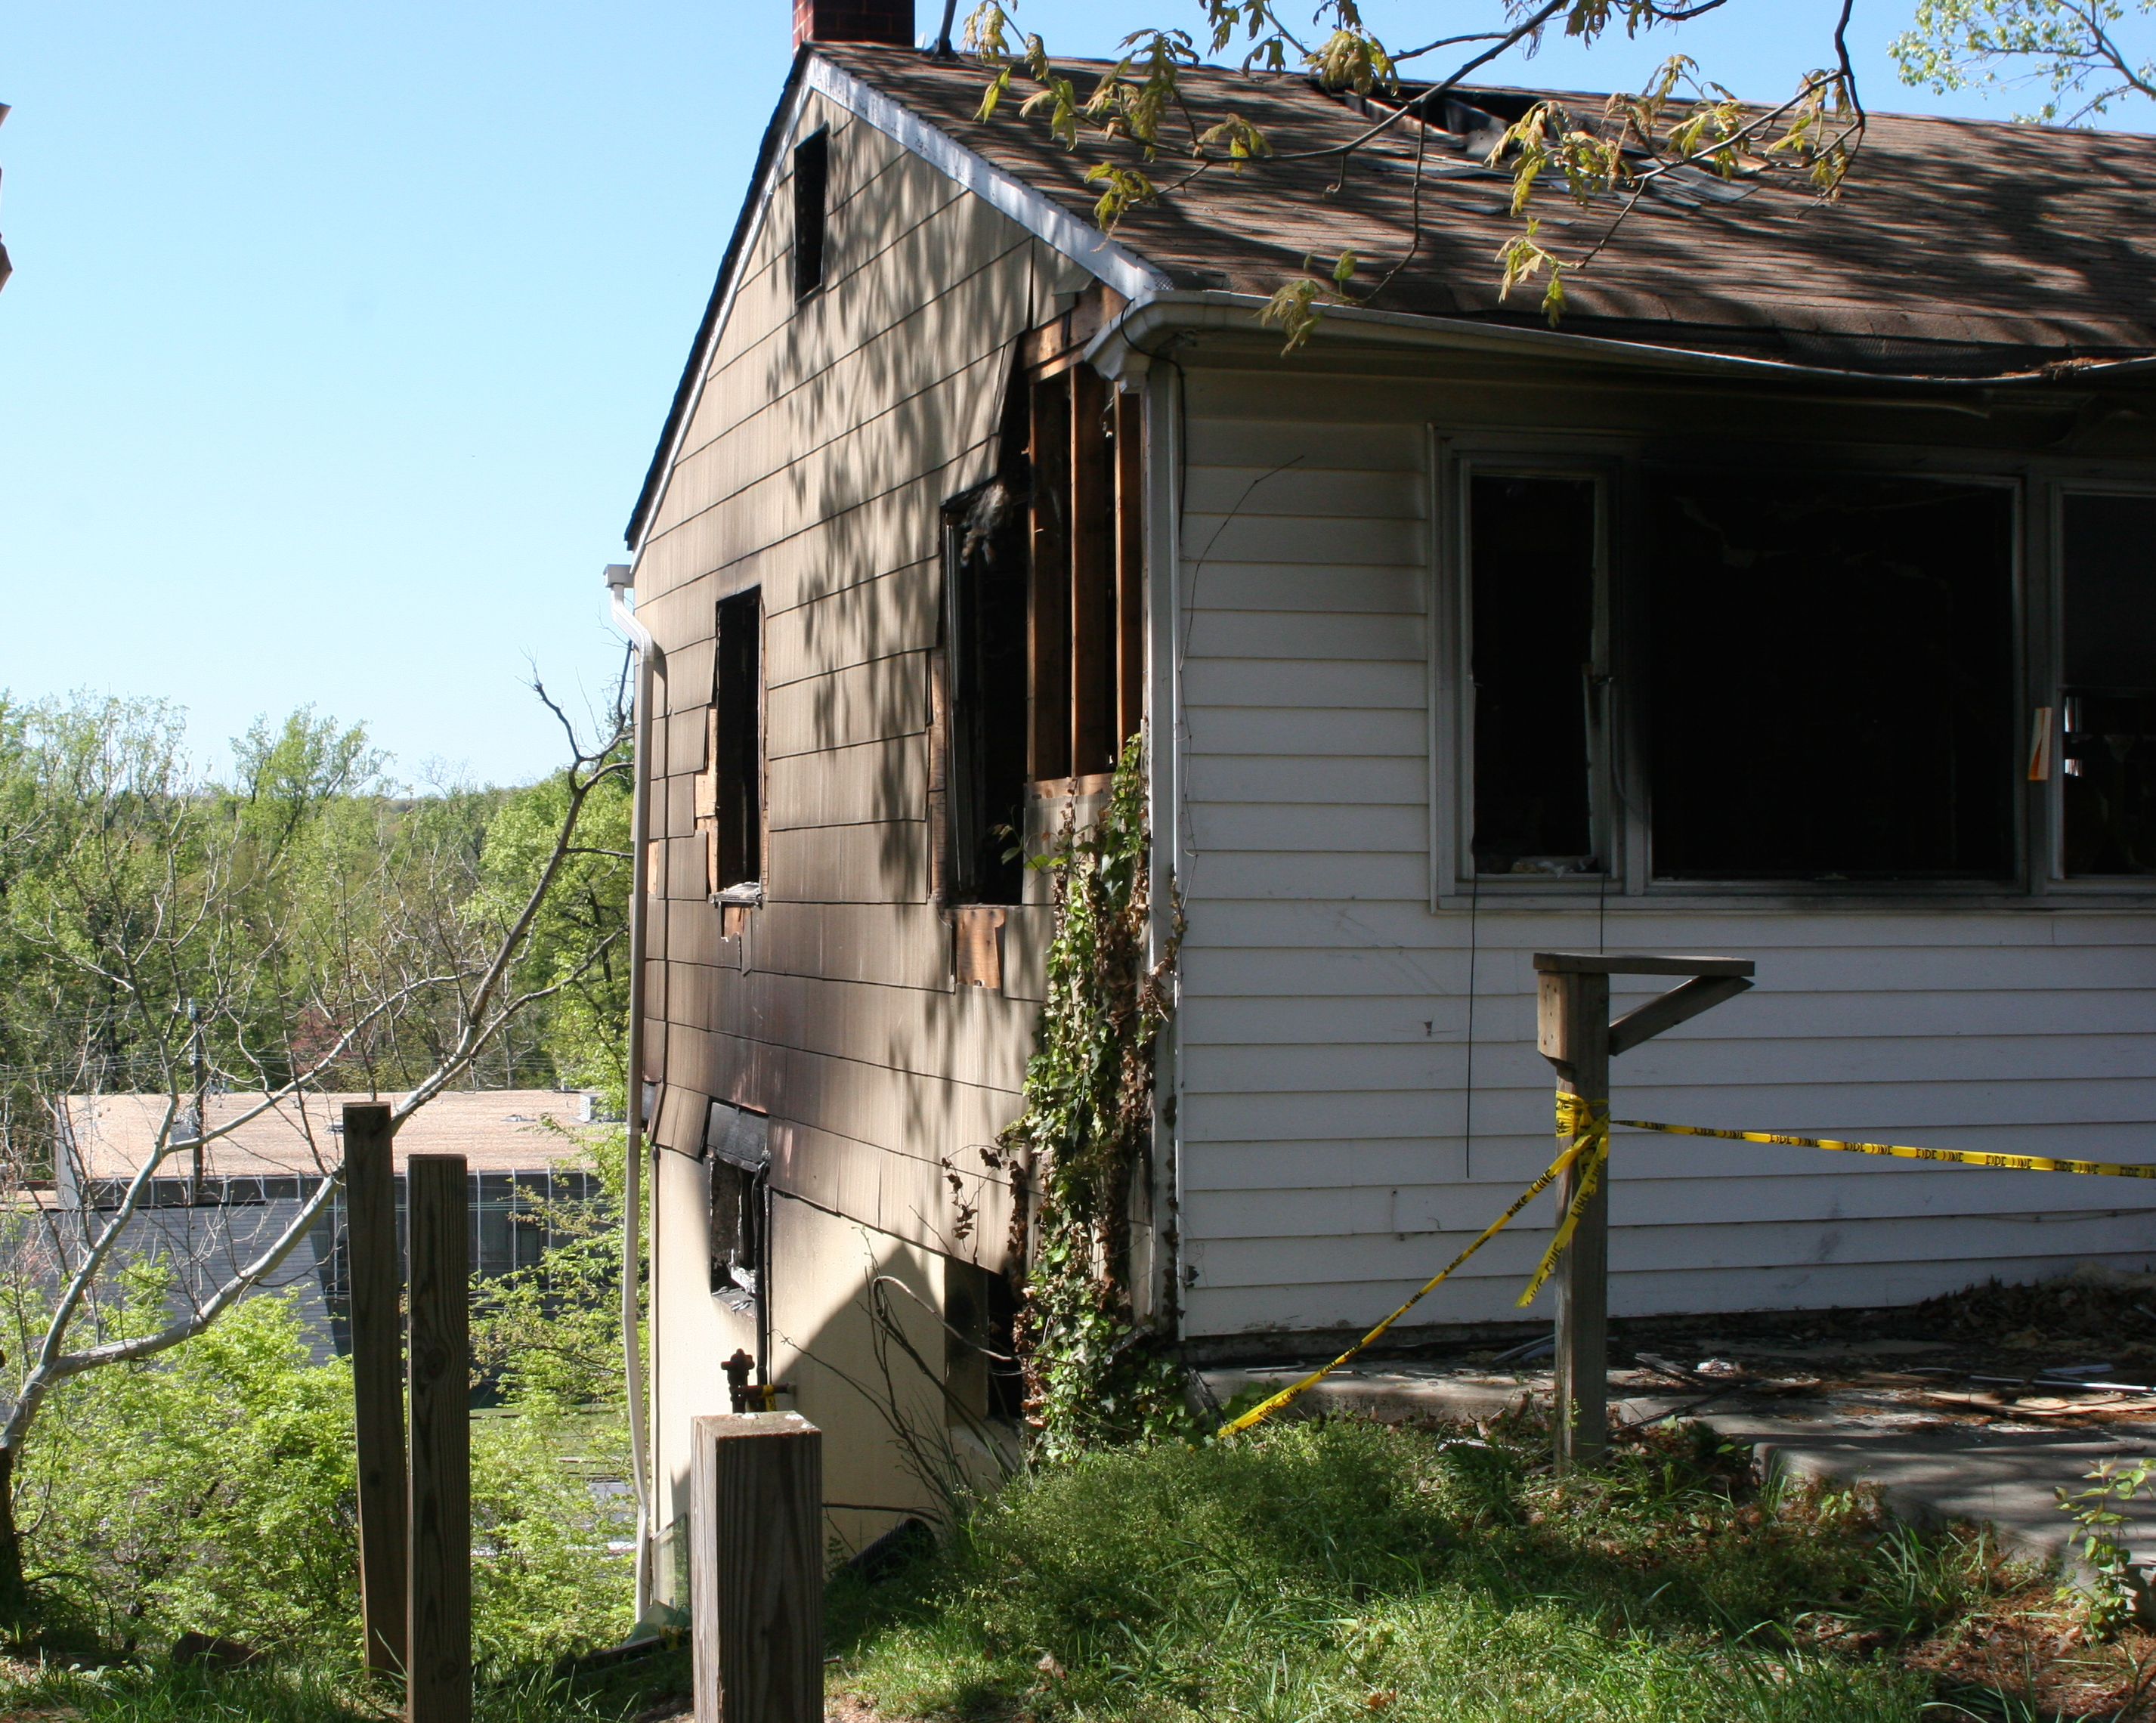
\includegraphics[width=.5\textwidth]{../Figures/PGCo_Slope}
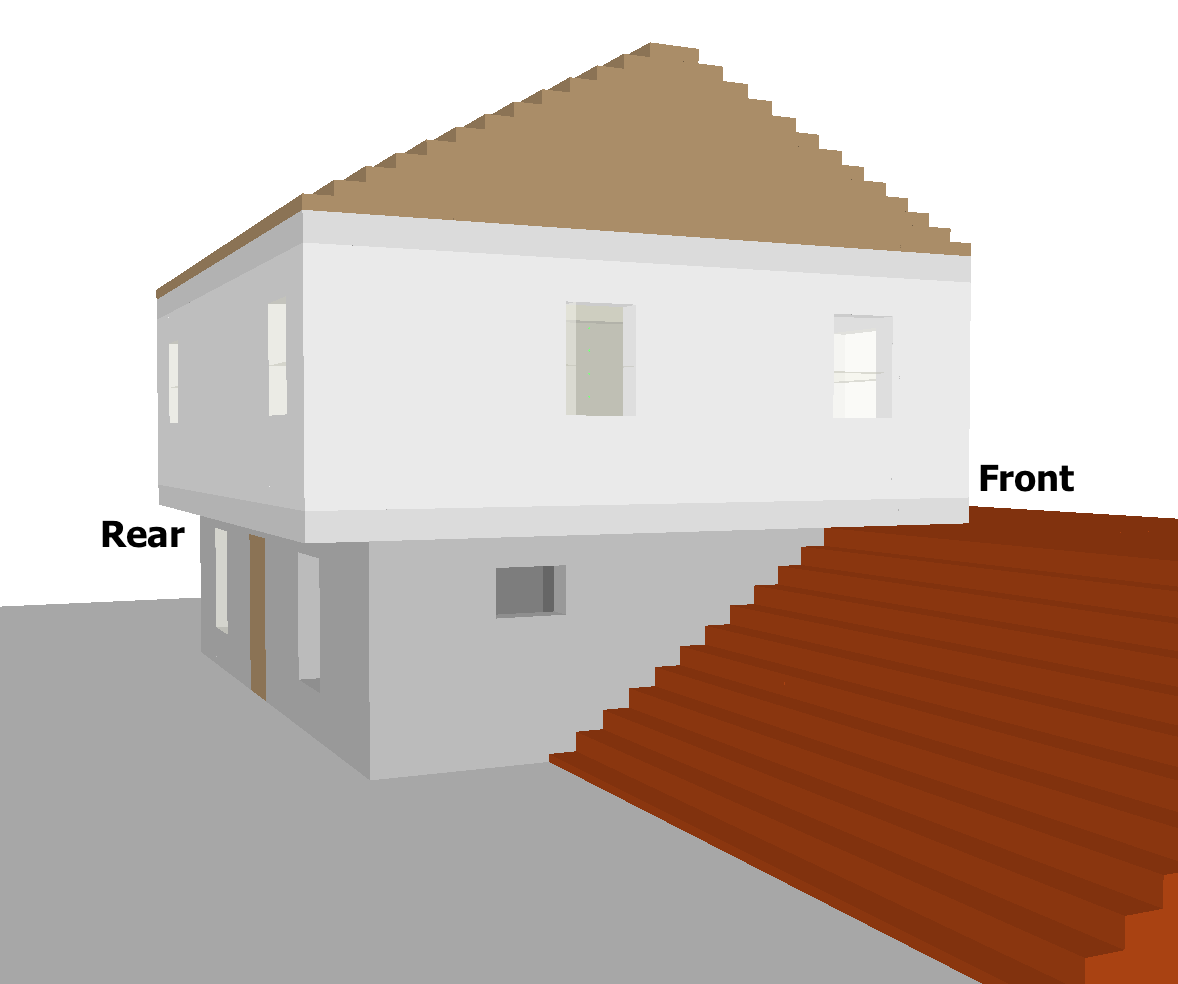
\includegraphics[width=.5\textwidth]{../Figures/pg_county_slope} \\
\caption[Photograph and computer model rendering of terrain.]{Photograph taken from front side street level showing the slope down to basement on the rear side of the structure (left) and Smokeview rendering of model representation of sloped landscape (right).}
\label{fig:slope}
\end{figure}

The fire, which is described in Section~\ref{fire}, started in the basement and spread to the stairs which connect to the first floor. Discussion of the fire's impact on the interior conditions is provided in Section~\ref{results}. Figure~\ref{fig:exterior} shows the exterior of the front and rear of the structure after the incident. Note that the majority of the damage occurred in the basement of the structure. Fully dimensioned drawings of the interior of the basement and first floor are shown in Figs.~\ref{fig:basement} and \ref{fig:first_floor}, respectively.

\begin{figure}[!ht]
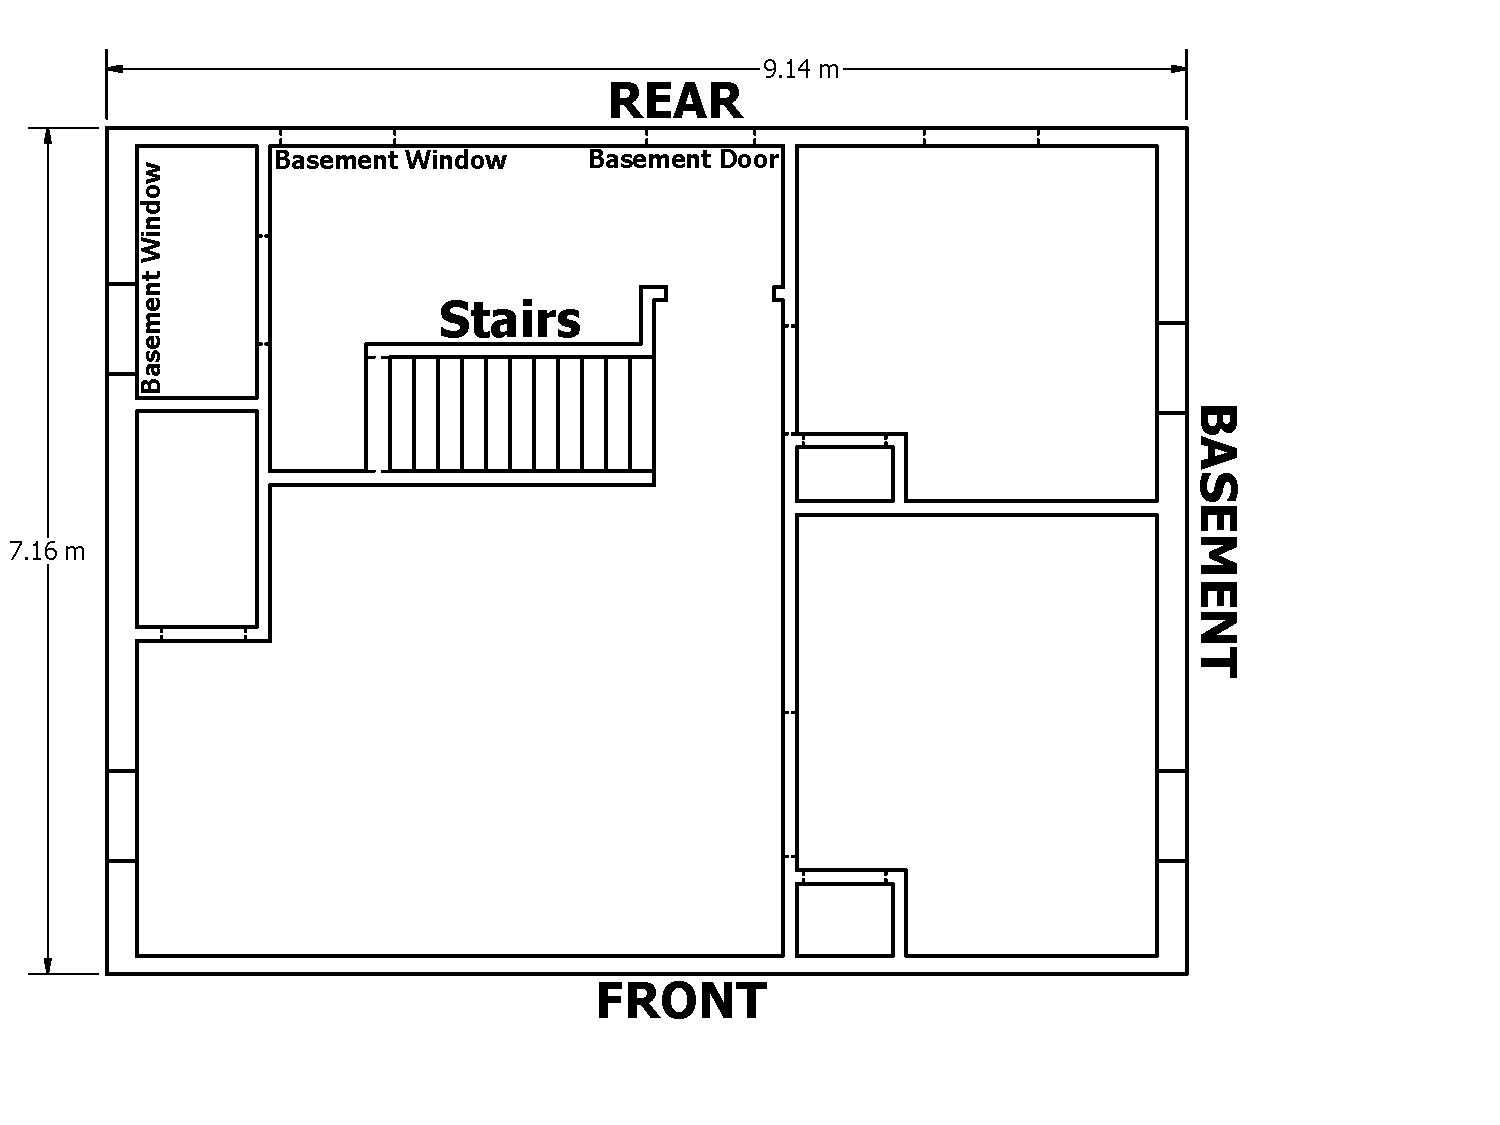
\includegraphics[width=.7\textwidth]{../Figures/Basement} \\
\vspace{0.2in}
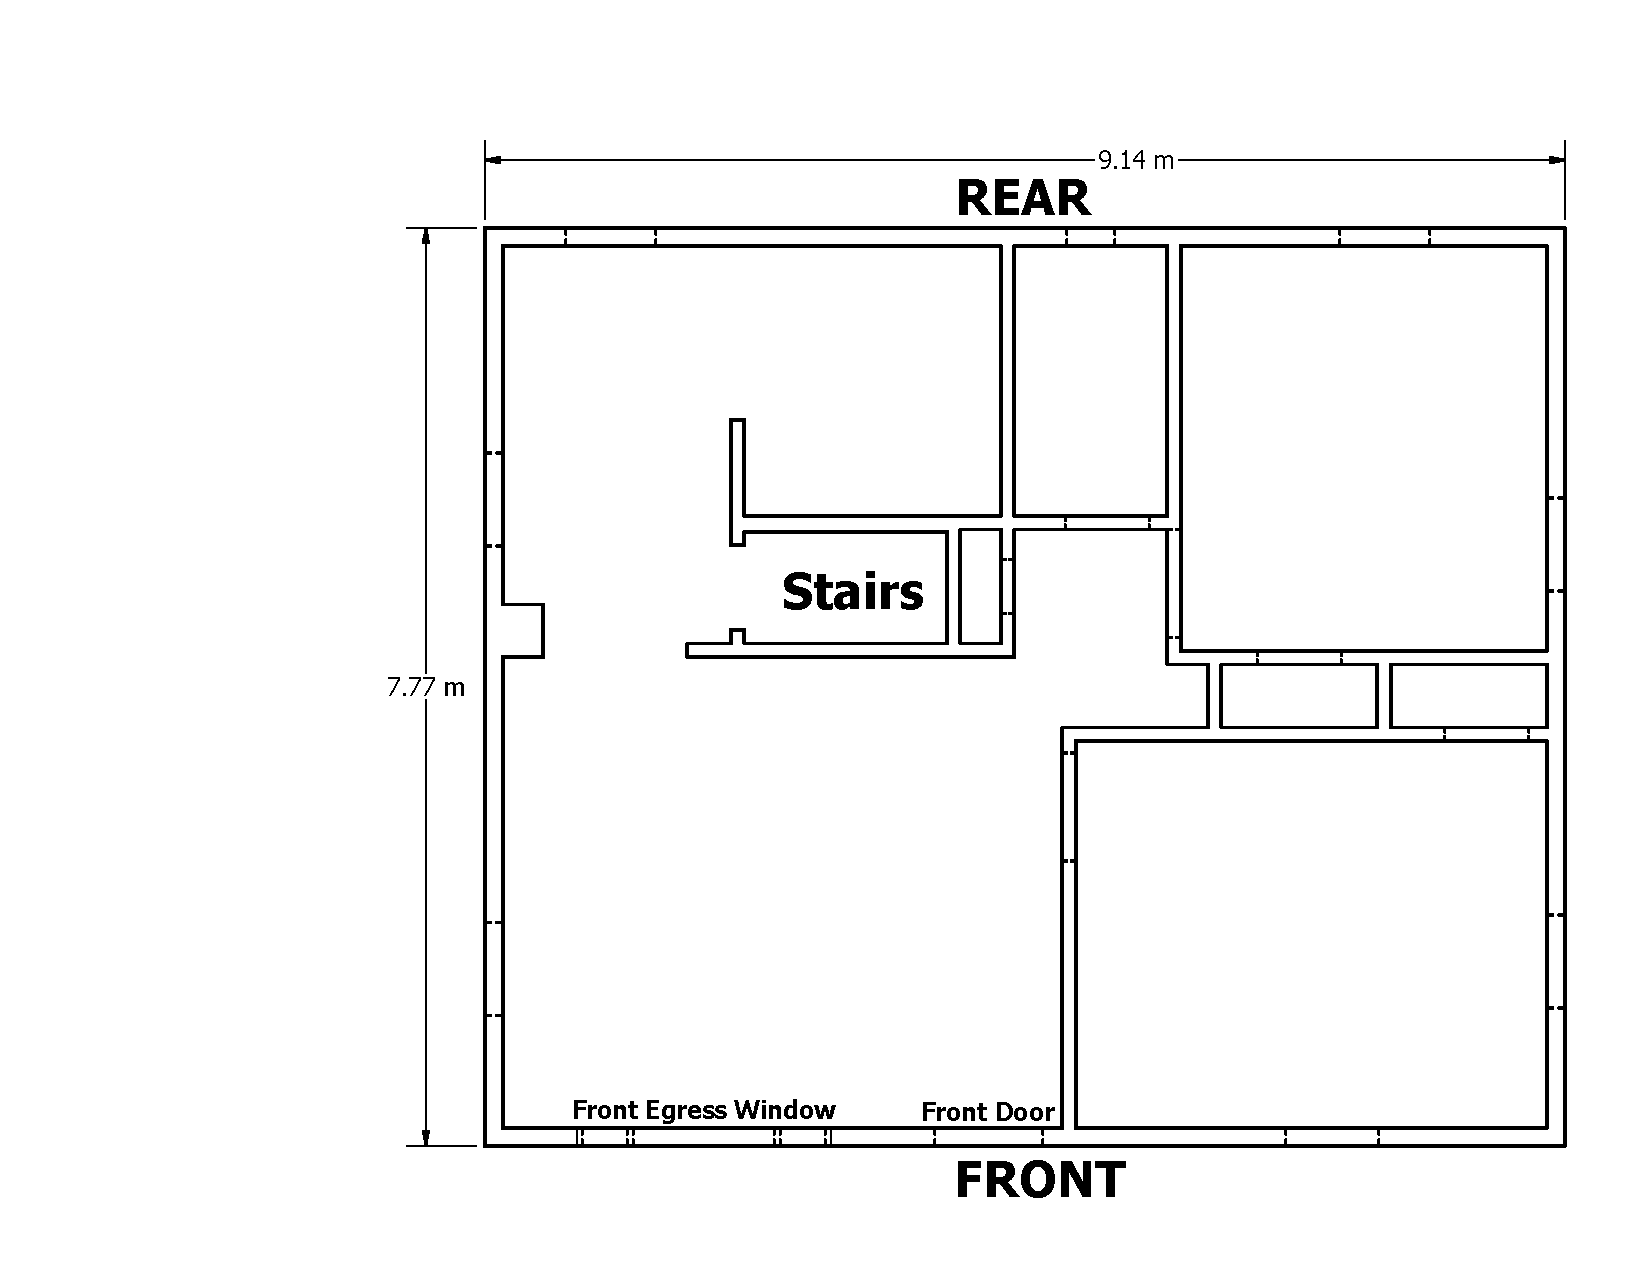
\includegraphics[width=.7\textwidth]{../Figures/First_Floor}
\caption[Plan view of basement (top) and first (bottom) floor of structure.]{Plan view of basement (top) and first (bottom) floor of structure. Stairs and key windows and doors are identified using measurements collected by NIST.}
\label{fig:simp_geom}
\end{figure}

\begin{figure}[!ht]
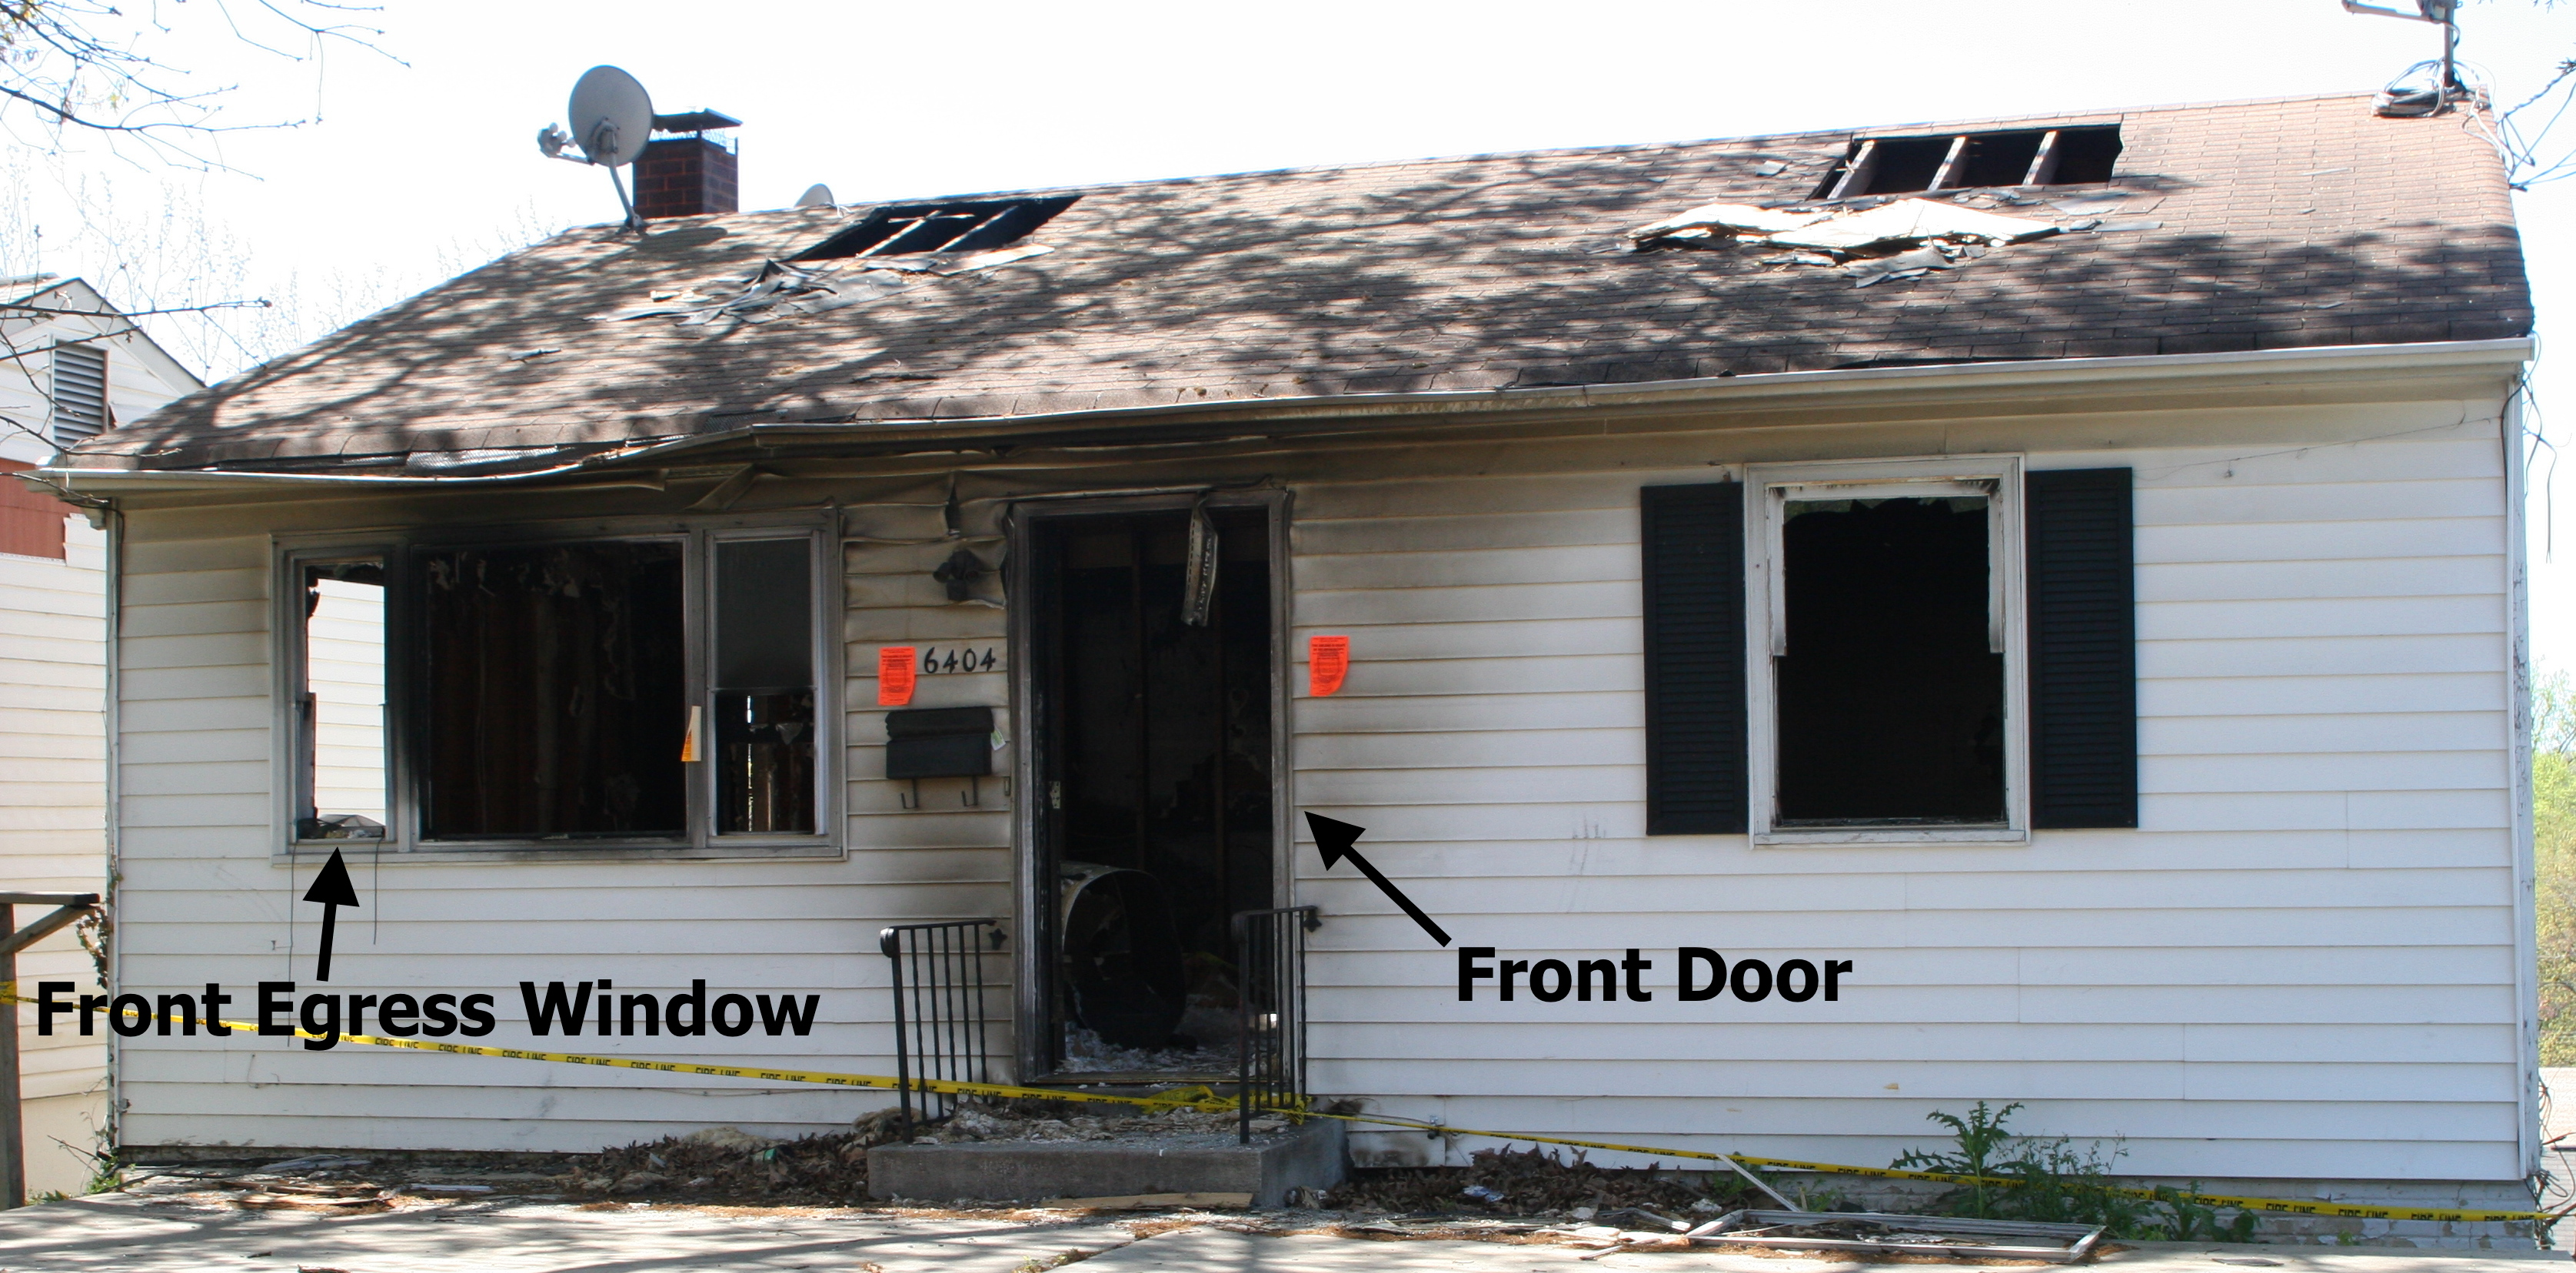
\includegraphics[width=5in]{../Figures/PGCo_Front} \\ 
\vspace{0.1in}
\includegraphics[width=5in]{../Figures/PGCo_Rear}
\caption{Photographs showing the front (top) and rear (bottom) exterior of the structure after the incident.}
\label{fig:exterior}
\end{figure}

\clearpage

\section{Fire}
\label{fire}
To estimate the type of fuel, fire size, and structure ventilation, on-scene videos and post-incident reports were used. Based on these sources of information, the FDS model includes two source fire locations in the basement: one fire in the kitchen area and one in the adjacent bathroom (Fig.~\ref{fig:basement_fire}). At the time of the fire, the structure was vacant so the the dominant fuel was wood: wood paneling on walls, exposed ceiling joists, sub-floor, cabinets, and stairs.

\begin{figure}[!ht]
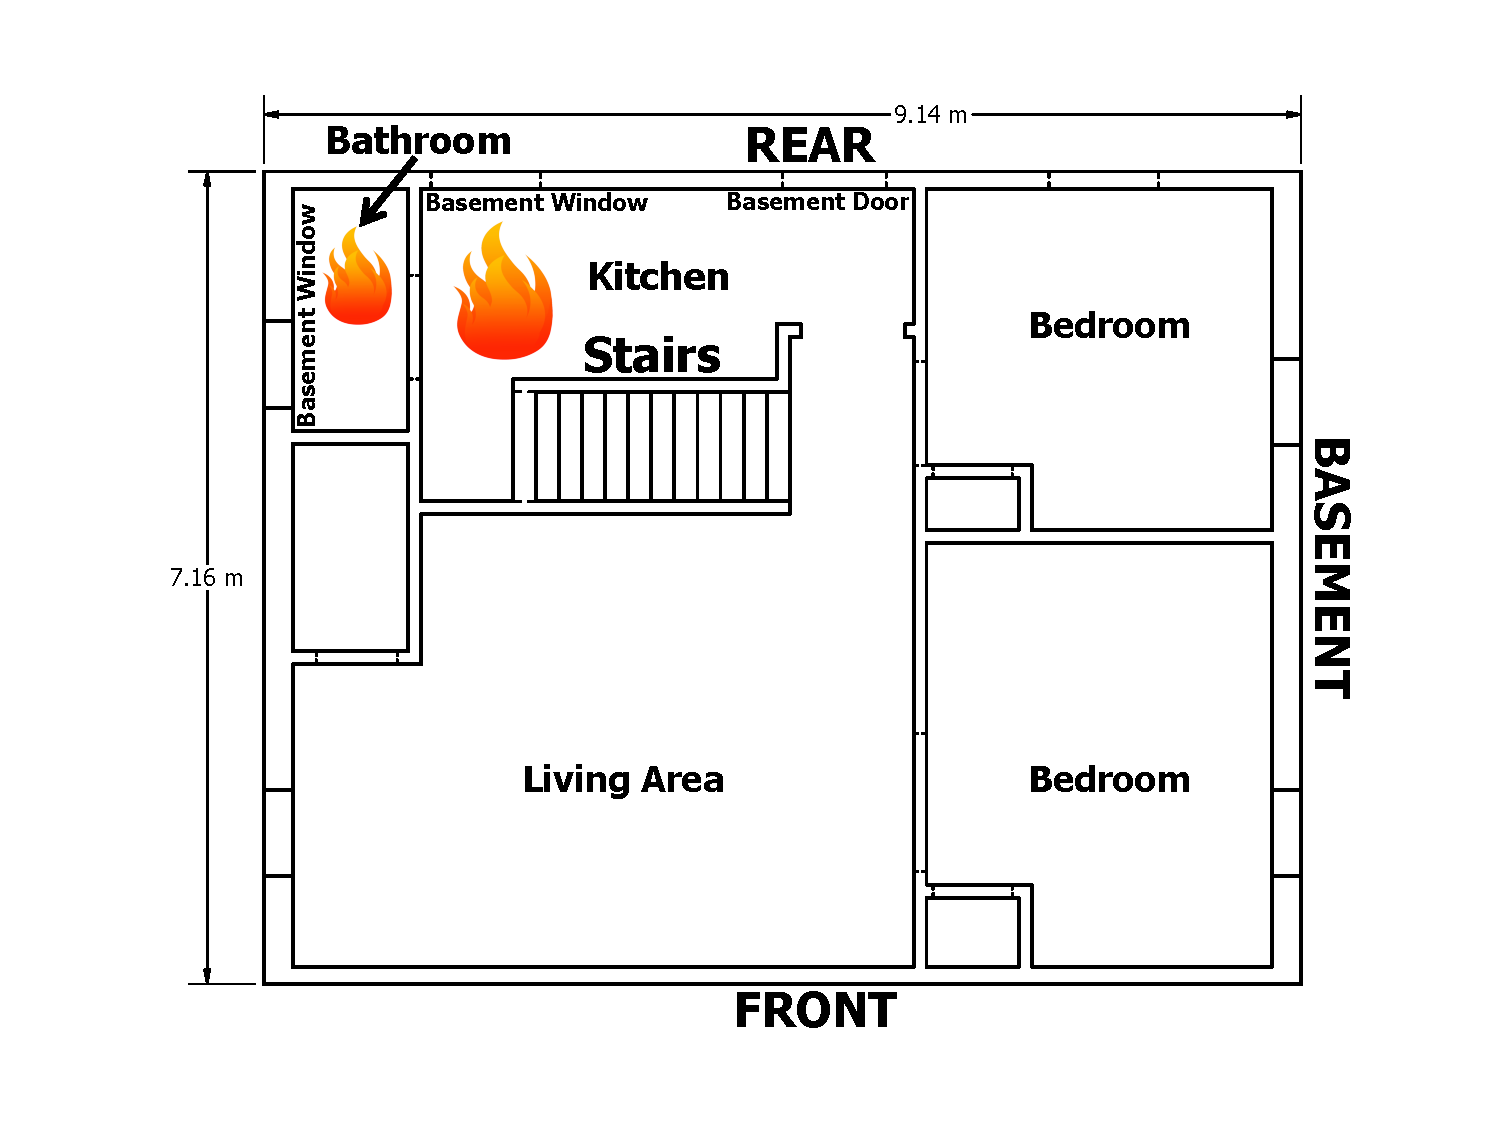
\includegraphics[width=0.8\textwidth]{../Figures/Basement_Fire}
\caption[Plan view of basement indicating fire location.]{Plan view of the basement indicating the location of the two fires in the FDS model.}
\label{fig:basement_fire}
\end{figure}


Wood fuel can be represented by the chemical formula, $\C\H_{1.7}\O_{0.74}\N_{0.002}$, with specified yields of carbon monoxide ($y_{\mathrm{CO}}=0.004 \; \mathrm{kg}/\mathrm{kg}$) and soot ($y_{\mathrm{C}}=0.015 \; \mathrm{kg}/\mathrm{kg}$)~\cite{SFPE:Tewarson}. The product yields are expressed in terms of the amount of carbon monoxide or soot emitted per unit mass of fuel consumed (kg/kg) and can be found in the Society of Fire Protection Engineers (SFPE) Handbook~\cite{SFPE:Tewarson}. A balanced chemical reaction for wood combustion can be written as:

\begin{multline}
\C\H_{1.7}\O_{0.74}\N_{0.002} + 4.91(0.208\,\O_{2} + 0.783\,\N_{2} + 0.387\text{\sc{e}-}3\,\C\O_{2} + 0.834\text{\sc{e}-}2\,\H_{2}\O) \\ 
\rightarrow 5.74(0.636\text{\sc{e}-}3\,\C\O + 0.168\,\C\O_{2} + 0.155\,\H_{2}\O + 0.670\,\N_{2} + 0.613\text{\sc{e}-}2\,\C)
\label{eq:wood_comb}
\end{multline}

The value for the heat of combustion of wood used in this simulation was~16,400 kJ/kg, based on data provided in the SFPE Handbook~\cite{SFPE:Tewarson}. The heat of combustion quantifies the amount of energy per unit mass of the fuel. The following text defines Eq.~\ref{eq:wood_comb} for an FDS input file with the desired fuel and reaction properties discussed above:

\begin{lstlisting}
&SPEC ID='WOOD', FORMULA='CH1.7O0.74N0.002' /

&REAC ID = 'wood' 
    FUEL = 'WOOD', 
    HEAT_OF_COMBUSTION = 16400,
    SOOT_YIELD = 0.015,
    CO_YIELD = 0.004/
\end{lstlisting}

Note that using the input lines above will invoke the simple chemistry reaction mechanism in FDS in which fuel and air react to form only CO$_2$, CO, H$_2$O, soot, and N$_2$. If the inclusion for other combustion products is desired, then the user must explicitly define those species and the chemical reaction that produces them~\cite{FDS_Users_Guide}. Based on the above input lines, FDS uses the default, mixing-controlled fast chemistry combustion model. This mechanism states that the rate of fuel consumption is proportional to both the local limiting reactant concentration and the local rate of mixing and extinction is based on the critical flame temperature approach~\cite{FDS_Math_Guide}. While FDS provides users with the option to use a more complex finite-rate combustion mechanism, there is not sufficient evidence in this case to justify deviating from the default specifications. 

To estimate the heat release rate per unit area (HRRPUA) of wood, Babrauskas and Grayson~\cite{babrauskas1990} conducted experiments in a cone calorimeter\footnote{The cone calorimeter is an experimental apparatus used to gather data about ignition time, mass loss, combustion products, and heat release rate among other properties associated with burning small samples of materials~\cite{ASTM:E1355}.} to determine the 5-min average of the HRRPUA for several different types of wood over a range of radiant heat fluxes. The results of that study indicate that the HRRPUA for different types of wood is approximately 50~kW/m$^2$.

To calculate the total fire size, the appropriate burning area of the basement needed to be determined. Based on the floor plan of the structure and post-incident images, two distinct fires were considered: 1 source in the basement bathroom and 1 source in the basement kitchen. 

Since the time at which the fire started is not known relative to the notification of a fire or how fast the fire spread, several simplifications were made. The fires started at the beginning of the simulation and increased to a value of 8.5~MW in 10~s. The 10-s ramp up time was used to prevent abrupt changes in the velocity at the fire boundary condition in FDS. Since the actual ignition time is unknown, the fire was ramped quickly to reflect the conditions determined from reports and post-incident images. The second assumption is that the sources of the gas phase wood fuel have constant areas at fixed locations in the basement (1 source for the kitchen, 1 source for the bathroom).  At 207~s, using a simple decay model, the fire size decreases lineraly to 25~\% of its peak value in 60~s. This is to account for the impact of firefighters putting water on the basement fire (Table~\ref{tab:fire_info}). The following lines define the source fires in the FDS input file:

\begin{lstlisting}
&SURF ID='burner1', HRRPUA = 2000, COLOR='BURNT ORANGE', RAMP_Q='BURN' /
&SURF ID='burner2', HRRPUA = 4500, COLOR='BURNT ORANGE', RAMP_Q='BURN' /

&RAMP ID='BURN', T = 0,   F = 0.  /
&RAMP ID='BURN', T = 10,  F = 1.0 /
&RAMP ID='BURN', T = 207, F = 1.0 /
&RAMP ID='BURN', T = 267, F = 0.25 /
&RAMP ID='BURN', T = 300, F = 0.25 /

&OBST XB=0.6,1.2,5,6.5,0.0,0.4, SURF_IDS='burner1','INERT','INERT' /  Burner1
&OBST XB=2.5,4,5.0,6.0,0.0,0.4, SURF_IDS='burner2','INERT','INERT' /  Burner2
\end{lstlisting}
Note that the coordinates here are unique for the vents are specific to the input files used for these simulations. The key point is the 2-D planar area. 

Figure~\ref{fig:hrr} shows the overall prescribed design fire for this scenario, which is the sum of the HRRs of the three source fires. In this figure, the text labels the prescribed steady peak HRR and the decay phase associated with firefighter water application. Therefore, the estimated maximum specified fire size for this structure was approximately 8.5~MW. Note that the prescribed HRR can be different than the simulated HRR calculated by FDS based on the amount of available fuel, oxygen, and ventilation. A comparison of the prescribed HRR and the simulated HRR is discussed in Section~\ref{HRR}.

\begin{figure}[!ht]
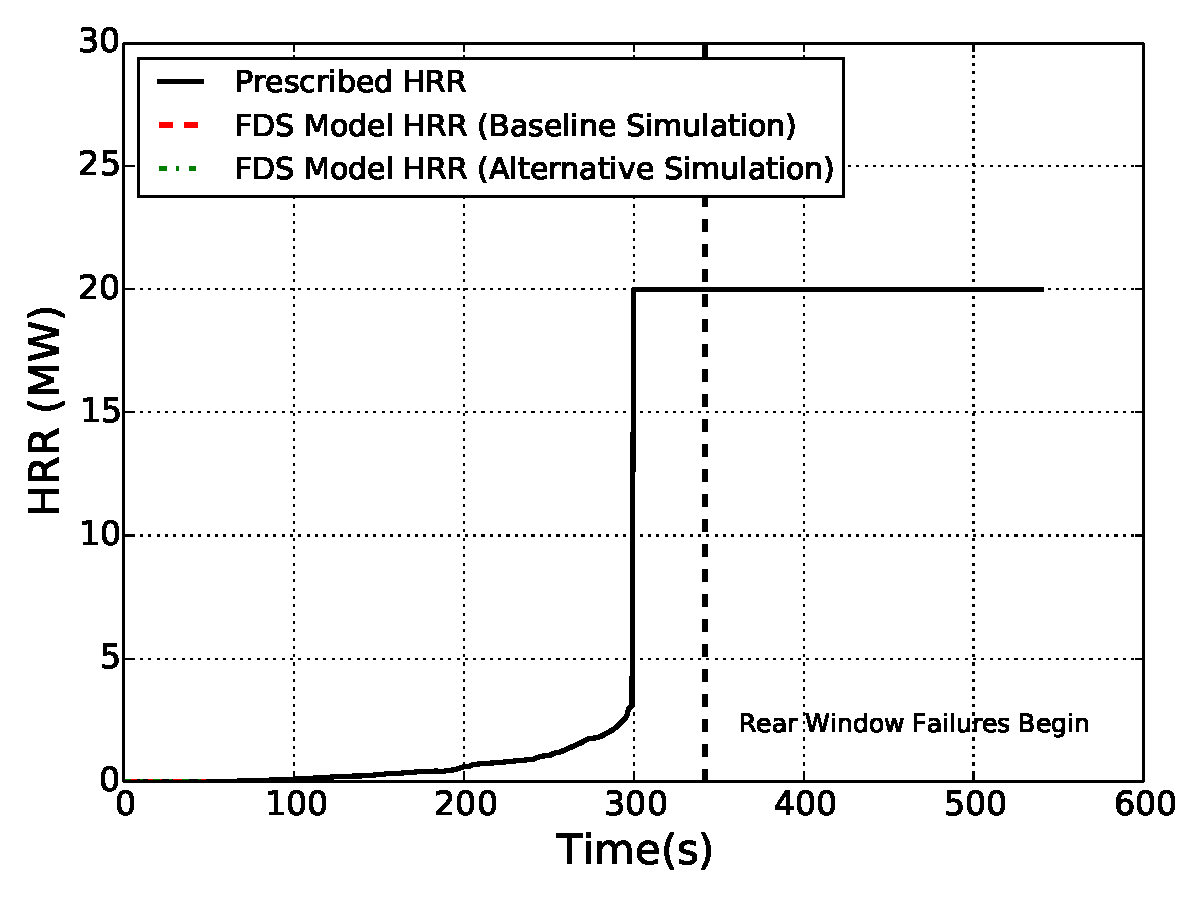
\includegraphics[width=0.75\textwidth]{../Figures/Fire_HRR}
\caption[Prescribed HRR vs. time for the simulation.]
{Prescribed HRR vs. time for the simulation. The text labels indicate the prescribed steady peak HRR and the decay phase associated with firefighter water application.}
\label{fig:hrr}
\end{figure}

\clearpage

\section{Materials}
\label{matl}
While the fires were represented as fuel sources with a constant area (Section~\ref{fire}), from a heat transfer perspective, it is important to define the material properties (density, thermal conductivity, and specific heat) to account for heat transfer and energy storage in the ceiling, walls, and floor. In this study, the material properties of gypsum board~\cite{WAKILI2007} were specified on the finished walls and ceilings on the main two floors of the structure, and the material properties of wood~\cite{Incropera:1} were specified on the unfinished portions of the attic and rear porch. The following lines define these materials in the FDS input file:

\begin{lstlisting}
&MATL ID = 'GYPSUM BOARD'
    FYI = 'Wakili - Journal of Fire Sciences 2007' 
    CONDUCTIVITY = 0.28
    SPECIFIC_HEAT = 1.0
    DENSITY = 810. /

&MATL ID = 'WOOD MAT'
    FYI = 'Incropera and DeWitt, Fundamentals of Heat and Mass Transfer'
    CONDUCTIVITY = 0.12
    SPECIFIC_HEAT = 1.38
    DENSITY = 510. / 
\end{lstlisting}

\section{Ventilation}
\label{Vents}
The simulations in this study account for changes in the ventilation due to a combination of fire department operations (opening doors, breaking windows), fire acting on the structure (fire breaching windows/doors) and wind (restricting flow, closing doors). The ventilation times and ventilation areas represent our best understanding of the incident. The times of ventilation changes for doors and windows are provided in Table~\ref{tab:vents}.

During the time at which the firefighters exited the structure or were rescued from the structure, the state of some windows and doors in the structure was known. The state of the vents (opened versus closed) resulted in the establishment of a flow path in the interior stairwell leading from the basement to the first floor. The exact time of operation for other doors/windows was not known. Therefore, the following the two basement windows on the left rear corner of the structure were assumed to be open at the start of the simulation. The states of the front door and front window were specified at certain times based on observations (i.e. forcible entry, wind effects, forced window breakage) from post-incident reports.

Structure leakage has been shown to be important when modeling enclosure fires~\cite{beal2009}. The open rear basement door and two open windows at the start of the simulation are significantly larger than the total effective area of leakage of a structure of this type. Therefore, any leakage in the structure would have a negligible impact on the fluid mechanics within the structure and is not included in this study.

In addition to the state of openings within the structure, outlined in Table~\ref{tab:vents}, an 8.9~m/s (20~mph) wind velocity boundary condition was included. The flow direction of the wind was from the rear toward the front of the structure, perpendicular to the rear of the structure.  Based on local weather conditions, mean wind velocities ranged between 4.5~m/s (10~mph) and 8.9~m/s (20~mph) with gusts up to 13.4~m/s (30~mph) with a direction that angled toward the back left of the structure~\cite{PGCounty2013}.

\begin{table}
\centering
\captionof{table}{Timeline of ventilation changes in the simulation}\label{tab:vents}
\begin{tabular}{lllll}
\toprule[1.5pt]
Baseline     &   Ventilation   &  Type       & State of       &  Side of  \\
Simulation  &  Area             &                 & Opening     &  Structure  \\
{[s]}             &  {[m$^2$]}     &                 &           &               \\
\midrule
0               &  1.40             &  Window      &  Opened     &  Rear  \\[.25cm]
0               &  0.39             &  Window      &  Opened     &  Left  \\[.25cm]
100             &  1.84             &  Door        &  Opened     &  Front \\[.25cm]
207             &  1.84             &  Door        &  Closed     &  Front \\[.25cm]
207             &  1.84             &  Door        &  Opened     &  Rear  \\[.25cm]
211             &  0.26             &  Window      &  Opened     &  Front \\[.25cm]
221             &  0.26             &  Window      &  Opened     &  Front \\[.25cm]
267             &  1.84             &  Door        &  Opened     &  Front \\[.25cm]

\bottomrule[1.25pt]
\end{tabular}\par
\footnotesize
\normalsize
\end{table}

\section{Numerical Mesh}
\label{mesh}
For the simulation, a measure of how well the flow field is resolved can be estimated by using the non-dimensional expression $D^*/\dx$. Here, $D^*$ is the characteristic fire diameter, $\dx$ is the nominal size of a mesh cell, and $\dQ$ is the total heat release rate of the fire:
\begin{equation}
D^* = \left(
     \frac{\dQ}{\rho_\infty \, c_p \, T_\infty \, \sqrt{g}}
     \right)^\frac{2}{5} 
\label{eq:mesh}
\end{equation}   
From the FDS User's Guide~\cite{FDS_Users_Guide}, the characteristic fire diameter is related to the characteristic fire size via the relation $Q^* = (D^*/D)^{5/2}$. Here, $D$ is the physical diameter of the base of the fire specified in the simulation. Following Eq.~\ref{eq:mesh} and using a grid cell size of 10~cm (3.9~in), the characteristic fire diameter to cell size ($D^*/\dx$) ratio is 12 for the 1.8~MW bathroom fire and 20 for the 6.75~MW basement fire. Based on validation work performed for the U.S. Nuclear Regulatory Commission, $D^*/\dx$ values ranged between 4 and 16~\cite{NUREG_1824} and produced results that were adequate for engineering calculations. The grid resolution used in this model is within or exceeds typical engineering $D^*/\dx$ values.

As discussed in Section~\ref{geom}, the structure has dimensions of 9.14~m (30~ft) by 7.62~m (25~ft) and a total height of 7.31~m (24~ft). To sufficiently resolve the wind boundary condtion, the computational domain was extended beyond the volume of the structure. The large domain led to the use of two separate grid resolutions, a 10~cm (3.9~in) resolution and a 20~cm (7.8~in) resolution. The 10~cm resolution encompasses the structure with a total volume 14~m (46~ft) by 12~m (39ft) by 8~m (26~ft) that required a total of 1.3 million computational cells. As a result, all of the input model geometry lengths, ventilation openings (holes, doors, and windows), and fire areas will snap to the nearest 10~cm. The 20~cm grid resolution extends the computational domain 5~m to the left and right sides and 4~m behind the 10~cm mesh to provide sufficient computational domain for the wind profile to develop around the structure. The mesh is coarser to cut down on computational time and because high accuracy in the fluid mechanics of the air flow far from the structure is not important in the analysis of this simulation. The 20~cm resolution resulted in an additional 216,000 computational cells.

Figure~\ref{fig:geom_grid} shows the front and rear of the structure and surrounding domain rendered in Smokeview with the 10~cm and 20~cm meshes. Note the finer mesh (smaller cells) surrounding the structure and the coarser mesh on each side. The domain was divided into 12 equally sized 10~cm meshes that surround the structure (each containing 150,000 grid cells) plus 4 equally sized 20~cm meshes to the left and right of the structure (each containing 32,000 grid cells) and one 20~cm mesh in the rear of the structure (containing 56,000 grid cells) for a total of 17 meshes. Multiple meshes allowed the simulation to be processed in parallel, which reduced the amount of required calculation time to approximately 3~days for the 20~mph wind case. Figure~\ref{fig:mult_mesh} shows the entire structure within the computational domain that has been divided into multiple meshes. The boundary between the twelve 10~cm meshes and five 20~cm meshes is indicated by the {\bf bold} lines. Table~\ref{tab:mod_param} shows a summary of the model input parameters for the simulations that were conducted as part of this study.

\begin{figure}[!ht]
\centering
\begin{tabular*}{\textwidth}{l@{\extracolsep{\fill}}r}
   \scalebox{1.0}{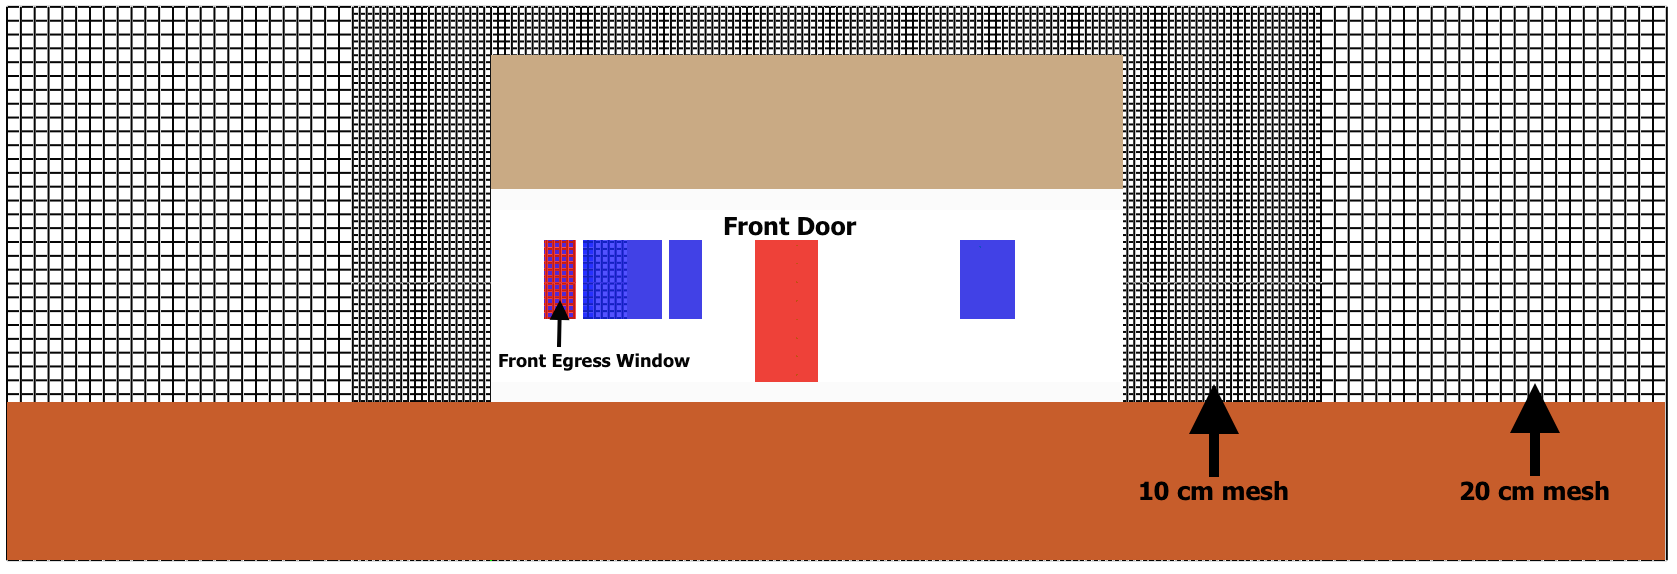
\includegraphics[width=\textwidth]{../Figures/pg_county_meshfront}} \\
   \scalebox{1.0}{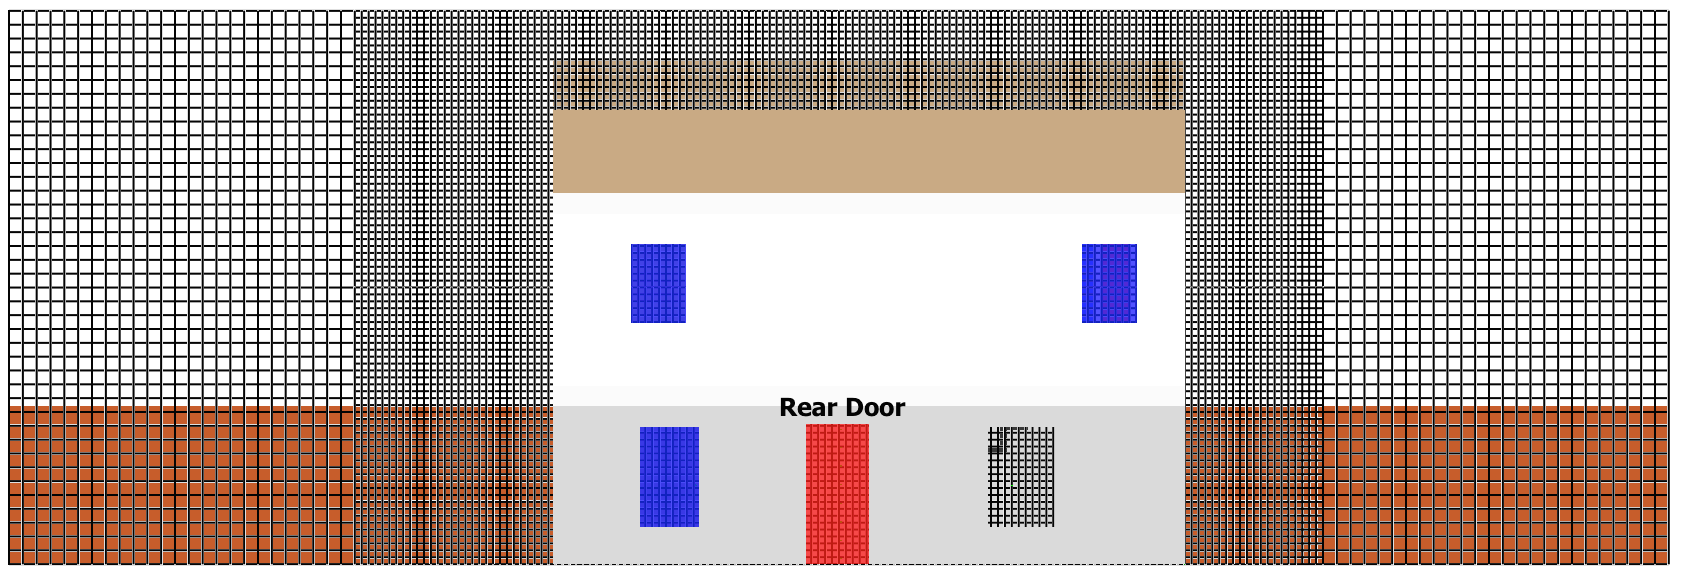
\includegraphics[width=\textwidth]{../Figures/pg_county_meshrear}} 
\end{tabular*}
\caption{Front (top) and rear (bottom) of the structure with 10~cm computational mesh surrounding the structure and 20~cm mesh to the left and right of the structure.}
\label{fig:geom_grid}
\end{figure}

\begin{figure}[!ht]
\centering
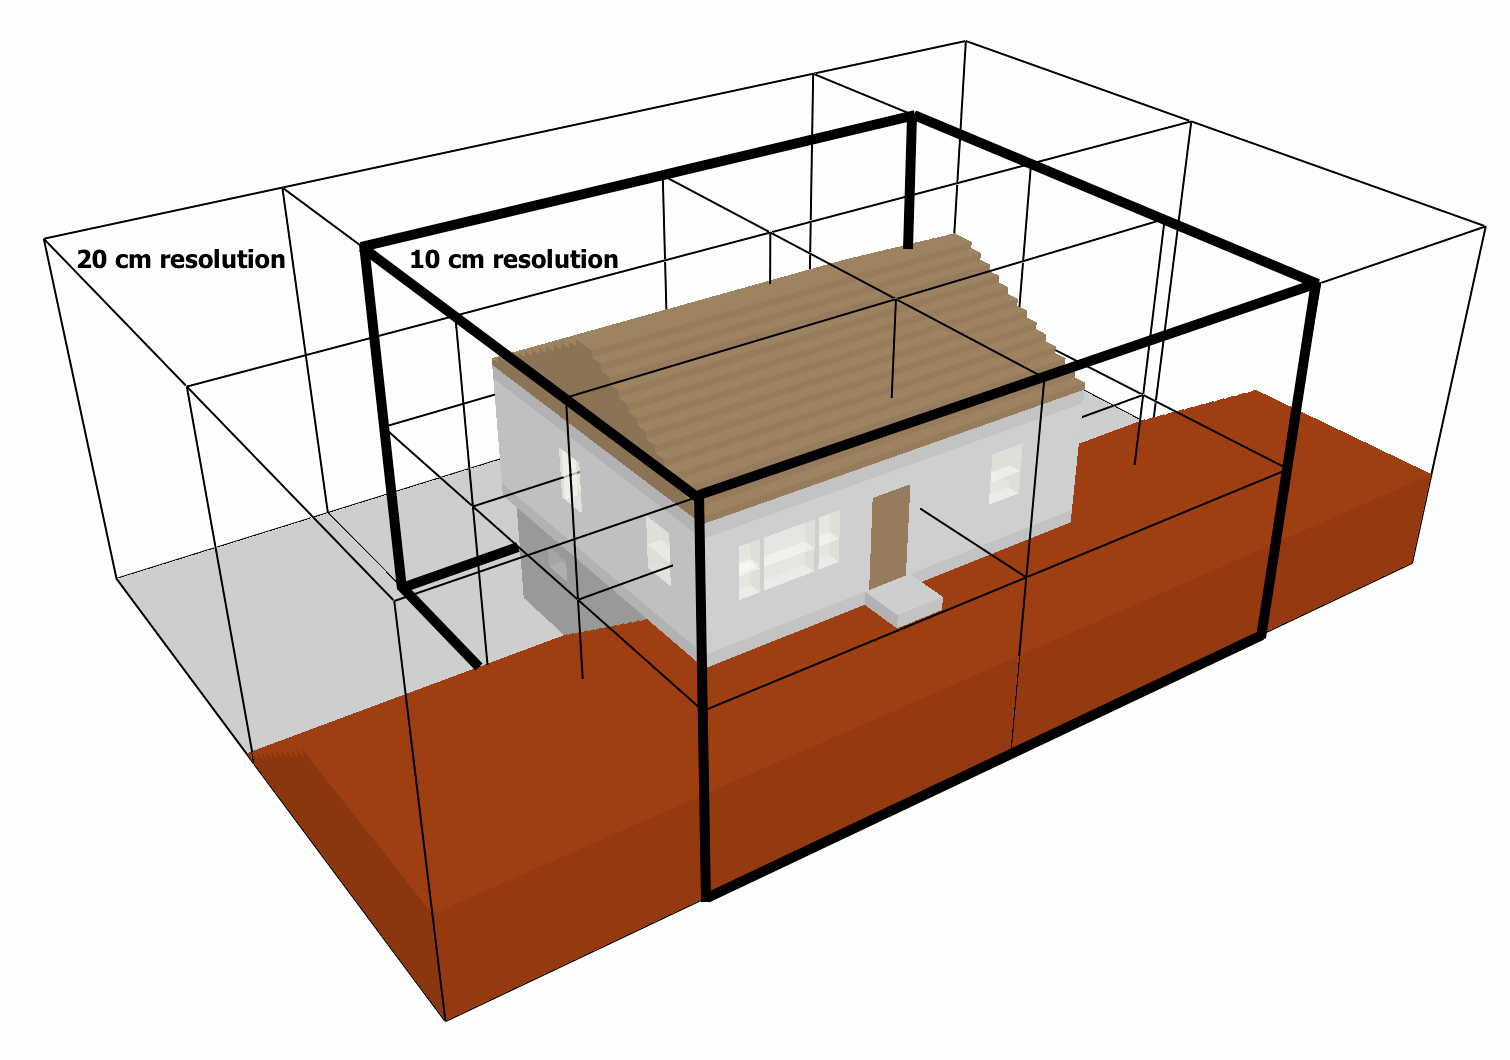
\includegraphics[width=\textwidth]{../Figures/pg_county_meshtotal2}
\caption[Overhead front-left side of the structure within the computational domain.]{Overhead front-left view of the structure within the computational domain (with 17 meshes). The entire computational domain is 24~m (79~ft) by 16~m (53~ft) by 8~m (26~ft).}
\label{fig:mult_mesh}
\end{figure}

\clearpage

\section{Summary of Model Input Parameters}
\label{sec:summary_of_model_inputs}

Table~\ref{tab:mod_param} shows a summary of the model input parameters for the simulation that was conducted as part of this study. In reality, the quantities associated with model input parameters are not fixed values; rather, a model input parameter can be thought of as a point estimate from a distribution of possible input parameters with some associated amount of uncertainty. Any change in an input parameter (such as the HRR) for a given scenario results in a change in the output quantity (such as the hot gas layer (HGL) temperature).

For example, according to the McCaffrey, Quintiere, and Harkleroad~\cite{SFPE:Walton} empirical correlation, the HGL temperature in a well-ventilated compartment fire is proportional to the HRR raised to the two-thirds power. Following this relationship, a 7.5~\% increase in the HRR would result in a 5~\% increase in the HGL temperature~\cite{NUREG_1824_Sup_1}. More detailed discussion on the propagation of parameter uncertainty in fire models is available in a validation study that was sponsored by the U.S. Nuclear Regulatory Commission~\cite{NUREG_1824_Sup_1}.


\begin{table}[!ht]
\centering
\captionof{table}{Relevant fire model input parameters}\label{tab:mod_param}
\begin{tabular}{lll}
\toprule[1.5pt]
Parameter                                                  & Description                                   & Discussion                            \\
\midrule
Simulation Time                                            &  5~min                                        & --                                    \\ [.25cm]
\multirow{2}{*}{Grid Cell Size}                            &  10~cm around house                           & \multirow{2}{*}{Section~\ref{mesh}}   \\ 
                                                           &  20~cm for wind                               &                                       \\ [.25cm]
Ambient Temperature$^*$                                    &  20~$^{\circ}$C (68~$^{\circ}$F)              & --                                    \\ [.1cm]
\multirow{4}{*}{Reaction: Wood~\cite{SFPE:Tewarson}}       &  Formula: $\C\H_{1.7}\O_{0.74}\N_{0.002}$     & \multirow{4}{*}{Section~\ref{fire}}   \\
                                                           &  CO Yield: 0.004~$\mathrm{kg}/\mathrm{kg}$    &                                       \\
                                                           &  Soot Yield: 0.015~$\mathrm{kg}/\mathrm{kg}$  &                                       \\
                                                           &  Heat of Combustion: 16,400~kJ/kg             &                                       \\ [.25cm]
\multirow{2}{*}{Peak HRR}                                  &  Basement Fire: 6.75~MW                       & \multirow{2}{*}{Section~\ref{fire}}   \\ 
                                                           &  Bathroom Fire: 1.8~MW                        &                                       \\ [.25cm]                     
\multirow{3}{*}{Material: Wood~\cite{Incropera:1} }        &  $k$: 0.12~\si{W/(m.K)})                      & \multirow{3}{*}{Section~\ref{matl}}   \\
                                                           &  $\rho$: 510~kg/m$^3$                         &                                       \\
                                                           &  $c_{p}$: 1.38~\si{kJ/(kg.K)}                 &                                       \\ [.25cm]
\multirow{3}{*}{Material: Gypsum Board~\cite{WAKILI2007}}  &  $k$: 0.28~\si{W/(m.K)}                       & \multirow{3}{*}{Section~\ref{matl}}   \\ 
                                                           &  $\rho$: 810~kg/m$^3$                         &                                       \\ 
                                                           &  $c_{p}$: 1.0~\si{kJ/(kg.K)}                  &                                       \\
\bottomrule[1.25pt]
\end{tabular}\par
\footnotesize
$^{*}$Initial interior temperatures were assumed to be 20~$^{\circ}$C; exterior temperatures were 10~$^{\circ}$C~\cite{PGCounty2013}.
\normalsize
\end{table}


\chapter{Model Results}
\label{results}

To examine the results of the simulation, it is important to link the timelines from the fire scene to the simulation times. Table~\ref{tab:combined_timeline} shows the fireground timeline~\cite{PGCounty2013} along with the corresponding simulation times.

\begin{table}[!ht]
\caption[Fire incident and simulation event timeline]
{Fire incident and simulation event timeline}
\begin{tabular}{ccl}
\toprule
Incident Time  &  Simulation  &  Fire Behavior / Fireground Operation                                \\
               &  Time        &                                                                      \\
{(hh:mm:ss)}   &  {(s)}       &                                                                      \\
\midrule
21:08:26       &              &  First 911 call is made.                                             \\
               &              &                                                                      \\
21:11:03       &              &  Dispatch for a``box'' alarm assignment- four engine companies       \\
               &              &  two truck companies, one rescue squad, and a commanding officer.    \\
               &              &                                                                      \\
21:21:20       &  0           &  FDS simulation begins.                                              \\
               &              &                                                                      \\
21:12:55       &              &  First unit (Engine 807B) arrived on-scene.                          \\
               &              &                                                                      \\
21:13:44       &              &  Volunteer Chief 809A establishes incident command (IC).             \\
               &              &                                                                      \\
21:13:56       &              &  Truck 809 arrived on-scene.                                         \\
               &              &                                                                      \\
21:14:00       &  100         &  Front door opened.                                                  \\
               &              &                                                                      \\
21:14:42       &              &  Truck 809 enters structure.                                         \\
               &              &                                                                      \\
21:15:47       &  207         &  Front door closed over.                                             \\
               &              &  Basement door opened and water applied to fire.                     \\
               &              &                                                                      \\
21:15:51       &  211         &  Lower pane of front egress window broke.                            \\
               &              &                                                                      \\
21:16:01       &  221         &  Top pane of front egress window broke.                              \\
               &              &                                                                      \\
21:16:16       &              &  Truck 809 officer bailout through window.                           \\
               &              &                                                                      \\
21:16:47       &  267         &  Front door opened.                                                  \\
               &              &                                                                      \\
21:17:15       &              &  Truck 809 forcible entry firefighter rescued.                       \\
               &              &                                                                      \\
\bottomrule
\end{tabular}
\footnotesize
\\ For specific information regarding ventilation areas used in the simulation, refer to Table~\ref{tab:vents}.
\normalsize
\label{tab:combined_timeline}
\end{table}

\clearpage

\section{Heat Release Rate}
\label{HRR}
In FDS, a HRR is specified, which results in a specified amount of fuel vapor (or pyrolyzate) being released from a fuel surface. FDS then determines the amount of combustion that occurs throughout the simulation based on the amount of available fuel and oxygen at a given location. As a result, the prescribed HRR that was input into the simulation can be different than the HRR calculated by FDS based on the ventilation conditions.

Figure~\ref{fig:PG_Total_HRR} shows the HRR in the structure vs. time based on the fires described in Section~\ref{fire}. In this figure, the solid line represents the prescribed HRR that was input into the simulation (based on a prescribed mass flux), and the dashed line represents the HRR inside the structure that was calculated by FDS based on the ventilation conditions. The vertical dashed lines represent the times at which ventilation occurred: front door opening and closing as well as the breaking of a front window for emergency escape. See Table~\ref{tab:vents} for a detailed list of the ventilation that occurring during the incident. The maximum size of the fire specified in this study was selected such that the conditions aligned with observations and fuel loads from the actual fire incident. 

\begin{figure}[!ht]
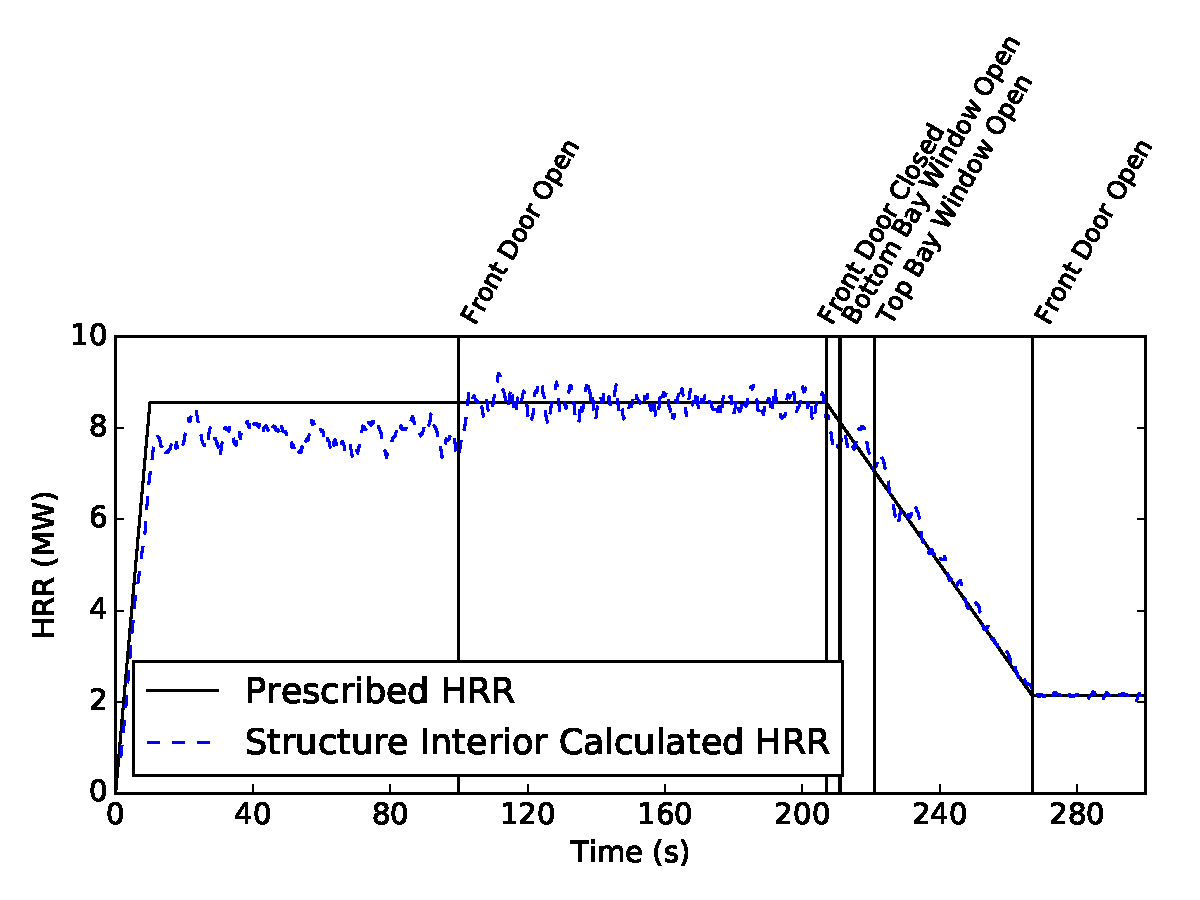
\includegraphics[width=5in]{../Figures/PG_Total_9MW_HRR}
\caption[Interior prescribed and calculated interior HRRs vs. time from the simulation.]
{Comparison of prescribed and calculated interior HRRs from the FDS simulation. The vertical lines indicate the times at which ventilation occurred.}
\label{fig:PG_Total_HRR}
\end{figure}

In Fig.~\ref{fig:PG_Total_HRR}, the prescribed HRR that was input into the simulation is different than the HRR calculated by FDS based on the ventilation conditions. From 0~s to approximately 9~s, the calculated HRR was in agreement with the prescribed HRR because there was an adequate amount of oxygen for all of the fuel to combust. The differences in prescribed versus predicted HRR is a result of either fuel within the structure accumulating and not combusting because of a lack of oxygen or combustion occurring exterior to the structure where fuel and oxygen can mix and react. Fig.~\ref{fig:PG_9MW_HRR} shows the total calculated HRR within the computational domain (includes combustion occurring exterior to the structure) compared to the prescribed HRR curve.

\begin{figure}[!ht]
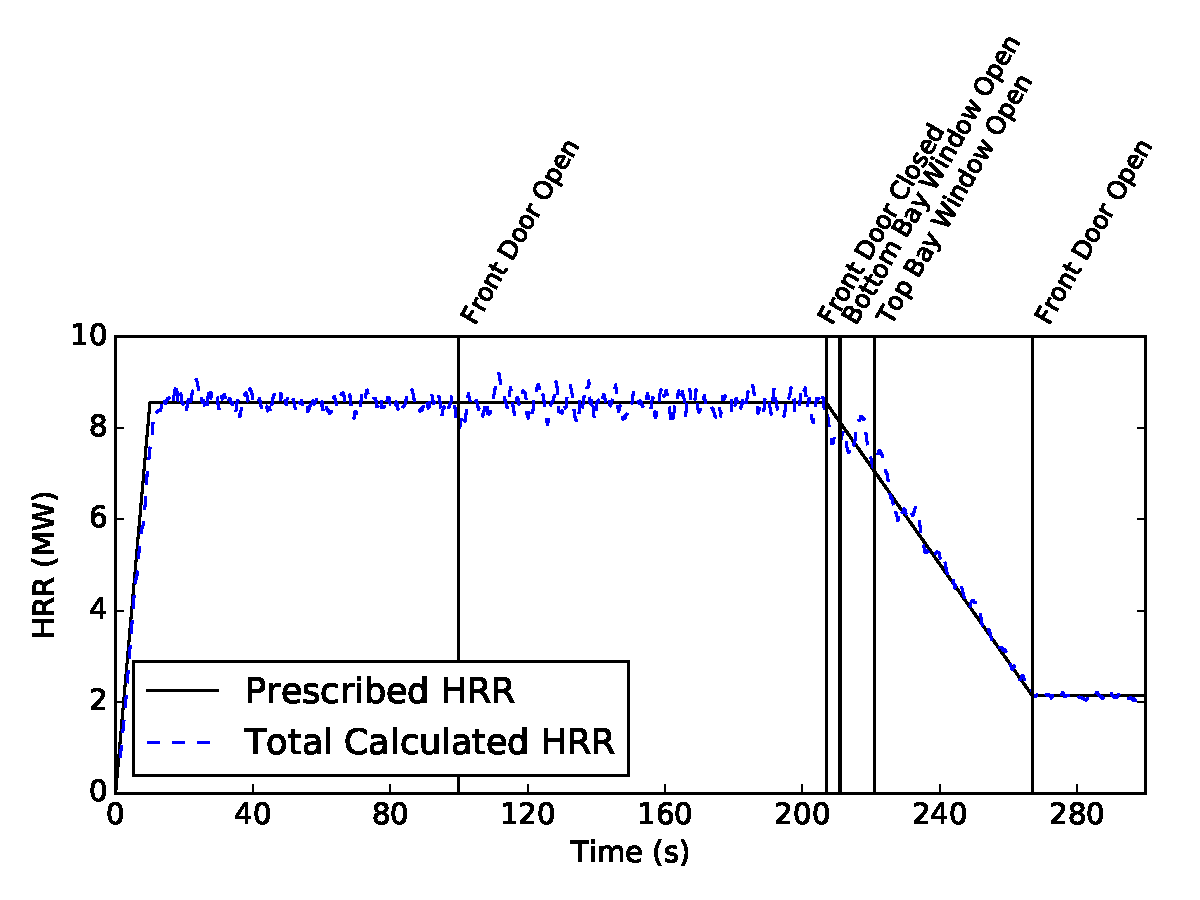
\includegraphics[width=5in]{../Figures/PG_9MW_HRR}
\caption[Prescribed and total calculated HRRs vs. time from the simulation.]
{Comparison of total prescribed and calculated HRRs within the entire computational domain from the FDS simulation. The vertical lines indicate the times at which ventilation occurred.}
\label{fig:PG_9MW_HRR}
\end{figure}

A comparison of the differences between the HRR inside the structure (Fig.~\ref{fig:PG_Total_HRR}) and the total HRR (Fig.~\ref{fig:PG_9MW_HRR}) over the first 100 seconds of the simulation indicates that on average there was the equivalent of an approximate 0.675 MW fire(s) occurring through open external vents. This aligns with observed post-fire damage and post-incident report~\cite{PGCounty2013}. Fig.~\ref{fig:ext_fire_dam} shows a post-fire image of the back left corner of the structure as well as a Smokeview rendering of the fire from the FDS simulation prior to the front door being opening by firefighters.

\begin{figure}[!ht]
\centering
\begin{tabular*}{\textwidth}{l@{\extracolsep{\fill}}r}
   \scalebox{1.0}{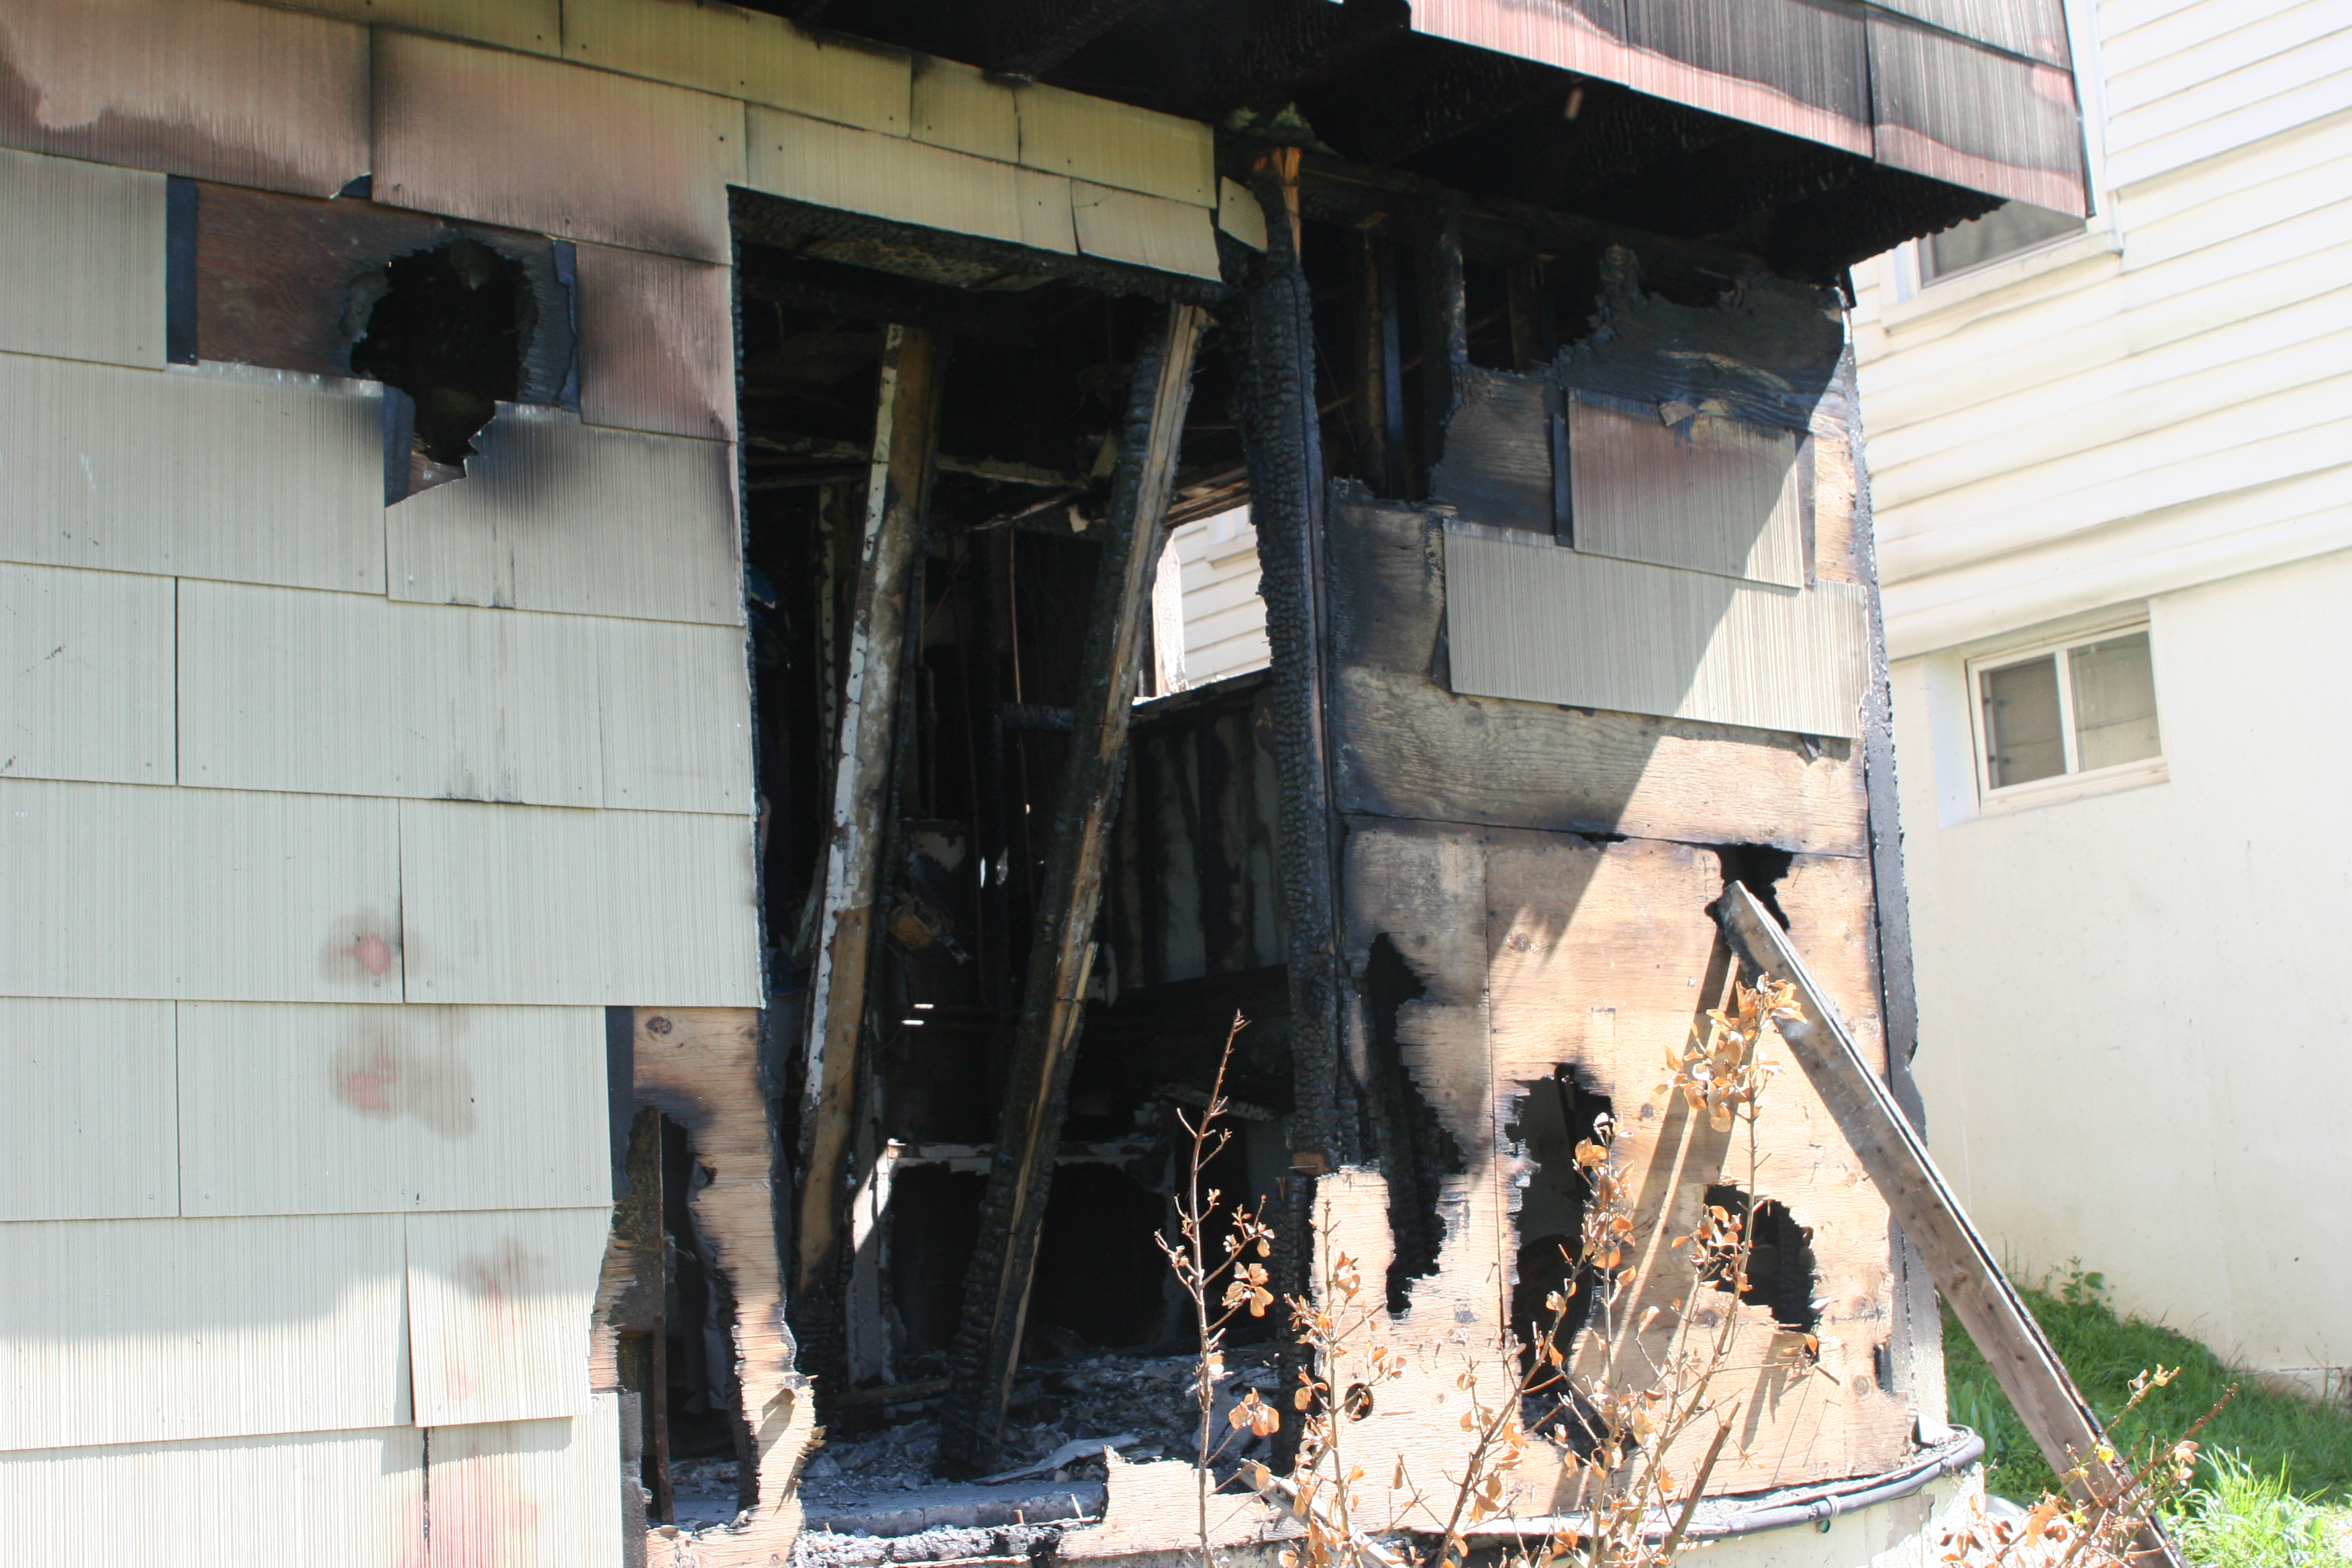
\includegraphics[width=.8\textwidth]{../Figures/Basement_External_Damage}} \\
   \scalebox{1.0}{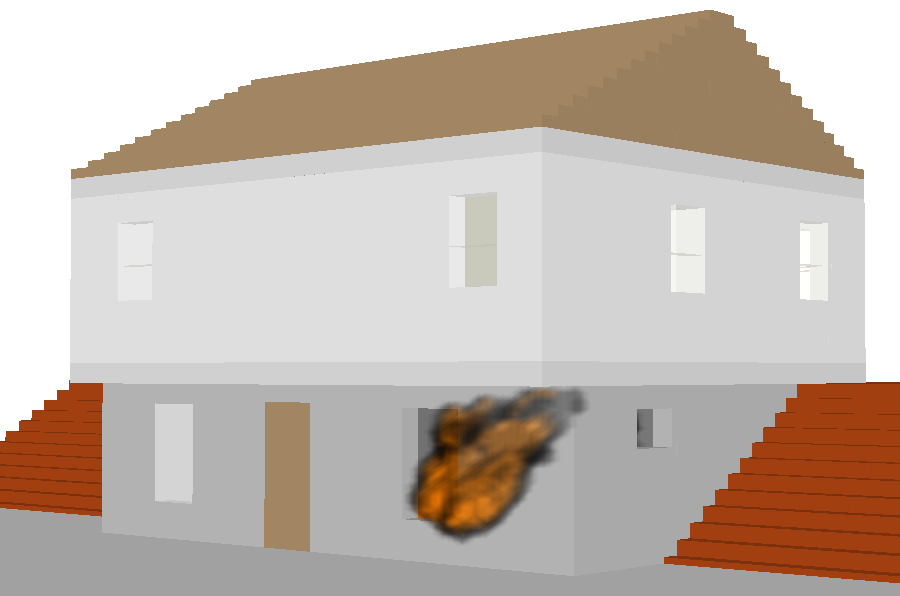
\includegraphics[width=.8\textwidth]{../Figures/Basement_FDS_Fire}} 
\end{tabular*}
\caption{External post-fire image of damage to the basement (top) and FDS model showing external fire prior to the front door of the structure being opened (bottom).}
\label{fig:ext_fire_dam}
\end{figure}

After 100 seconds of simulation time, 5~\sfrac{1}{2}~minutes after the first 911 call, firefighters open the front door to make entry to the first floor of the structure. The change in ventilation to the structure impacted the HRR. After the door was opened, combustion no longer tool place outside of the structure, however as shown in Fig.~\ref{fig:PG_Basement_9MW_HRR}, the basement HRR was lower than the total HRR within the domain.

\begin{figure}[!ht]
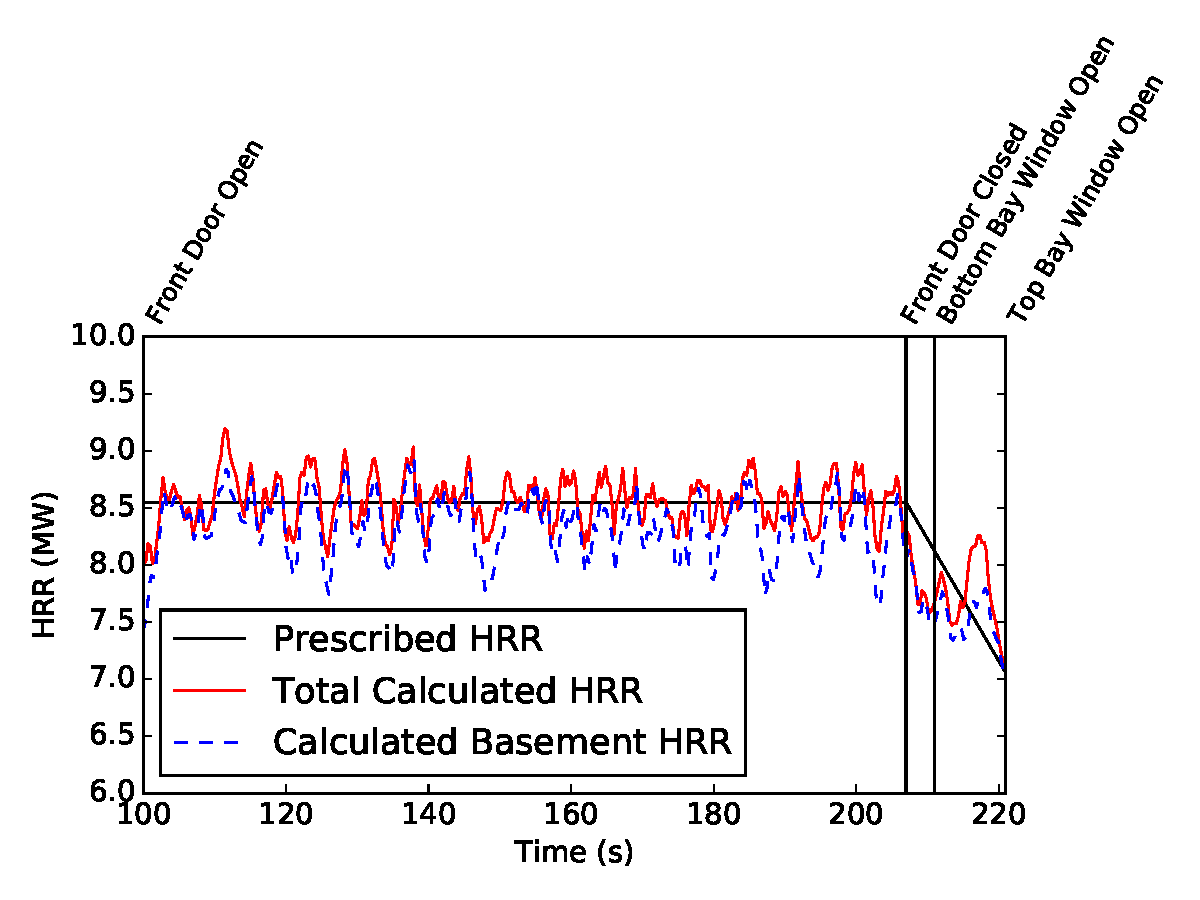
\includegraphics[width=5in]{../Figures/PG_Basement_9MW_HRR}
\caption[Prescribed, calculated domain, and calculated basement HRRs vs. time from the simulation.]
{Comparison of prescribed, total calculated domain HRR and basement calculated HRRs from the simulation. The vertical lines indicate the times at which ventilation occurred.}
\label{fig:PG_Basement_9MW_HRR}
\end{figure}

The differences in HRR between the total HRR and the basement HRR can be accounted for in combustion occurring on the first floor of the structure. Fuel that was combusting outside of the structure due to a lack of oxygen combusts on the first floor of the structure as the open front door allows flow to occur within the structure and fuel to mix with available oxygen and react (Fig.~\ref{fig:PG_First_9MW_HRR}).

\begin{figure}[!ht]
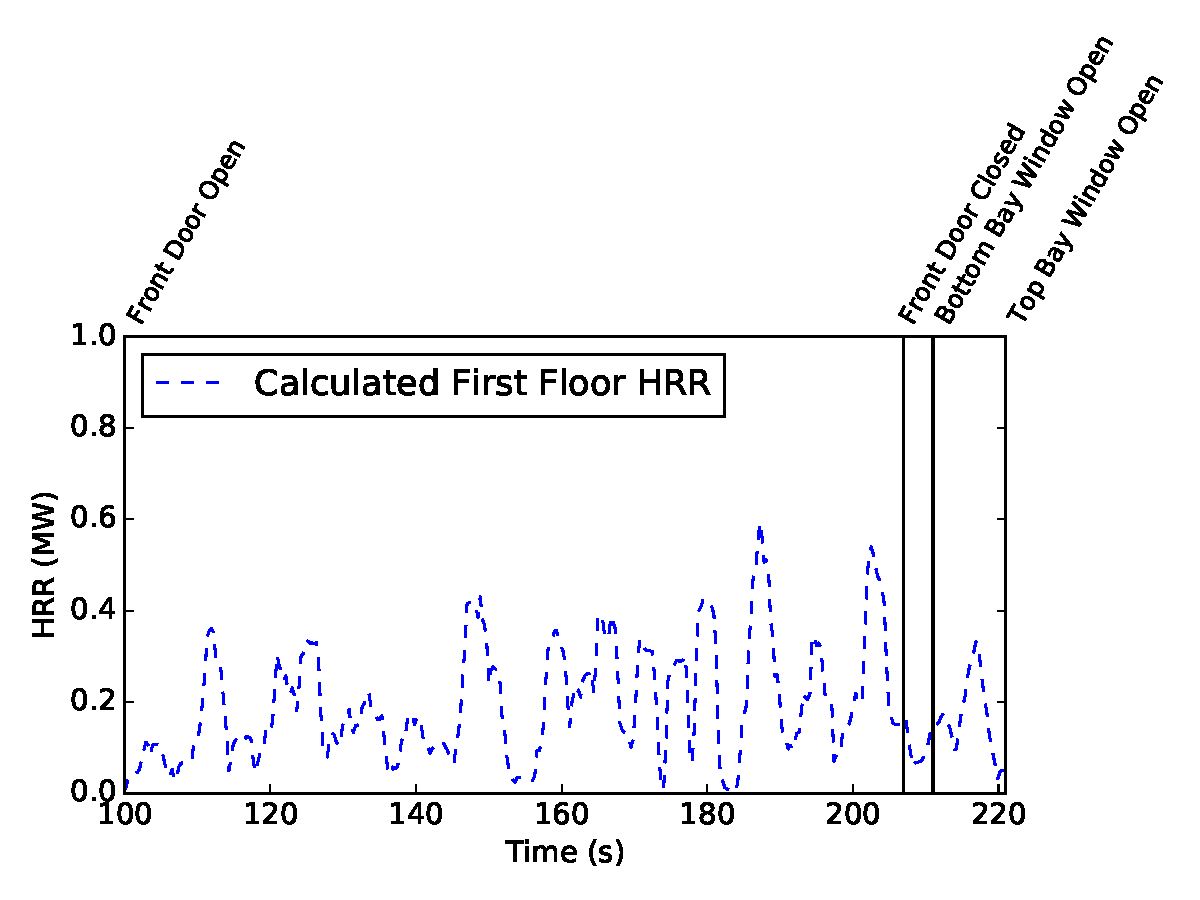
\includegraphics[width=5in]{../Figures/PG_First_9MW_HRR}
\caption[Prescribed and first floor calculated HRR vs. time from the simulation.]
{Comparison of total prescribed and first floor calculated HRRs from the simulation. The vertical lines indicate the times at which ventilation occurred.}
\label{fig:PG_First_9MW_HRR}
\end{figure}

\clearpage

\section{Pressure}
\label{pressure}

The growth of the fire combined with a 8.9~m/s (20~mph) wind flowing normal to the rear of the structure caused the pressure to rise within the structure. Hot gases which may have built up within the structure will flow from high pressure to low pressure. Based on the event timeline, the front door was opened 100 seconds into the simulation, which would create a low pressure relief on the first floor. Due to firefighters entering the structure through the front door, the simulated pressure in the first floor prior to and just after opening the door is important. Figure~\ref{fig:pressure_slices} shows the calculated pressure conditions in the structure just before and after the front door was opened (100~s) in the simulation.

In the top snapshot in Fig.~\ref{fig:pressure_slices}, the pressure profile shows an overpressure of approximately 200~Pa (2.9 $\times$ 10$^{-2}$~psi) prior to the door being opened. This pressure may be on the conservative side (over-prediction) because of wind speed fluctuations, wind direction, and small amounts of structure leakage. One second after the door was opened (bottom snapshot in Fig.~\ref{fig:pressure_slices}), the pressure on the first floor drops to between 75~Pa (1.1 $\times$ 10$^{-2}$~psi) and 85~Pa (1.2 $\times$ 10$^{-2}$~psi). Without the presence of wind, the pressure in the first floor prior to the door opening is is approximately 18~Pa (2.6 $\times$ 10$^{-3}$~psi) and after the door is opened the pressure drops to between 5~Pa (7.3 $\times$ 10$^{-4}$~psi) and 10~Pa (1.4 $\times$ 10$^{-3}$~psi).

\clearpage

\begin{figure}[!ht]
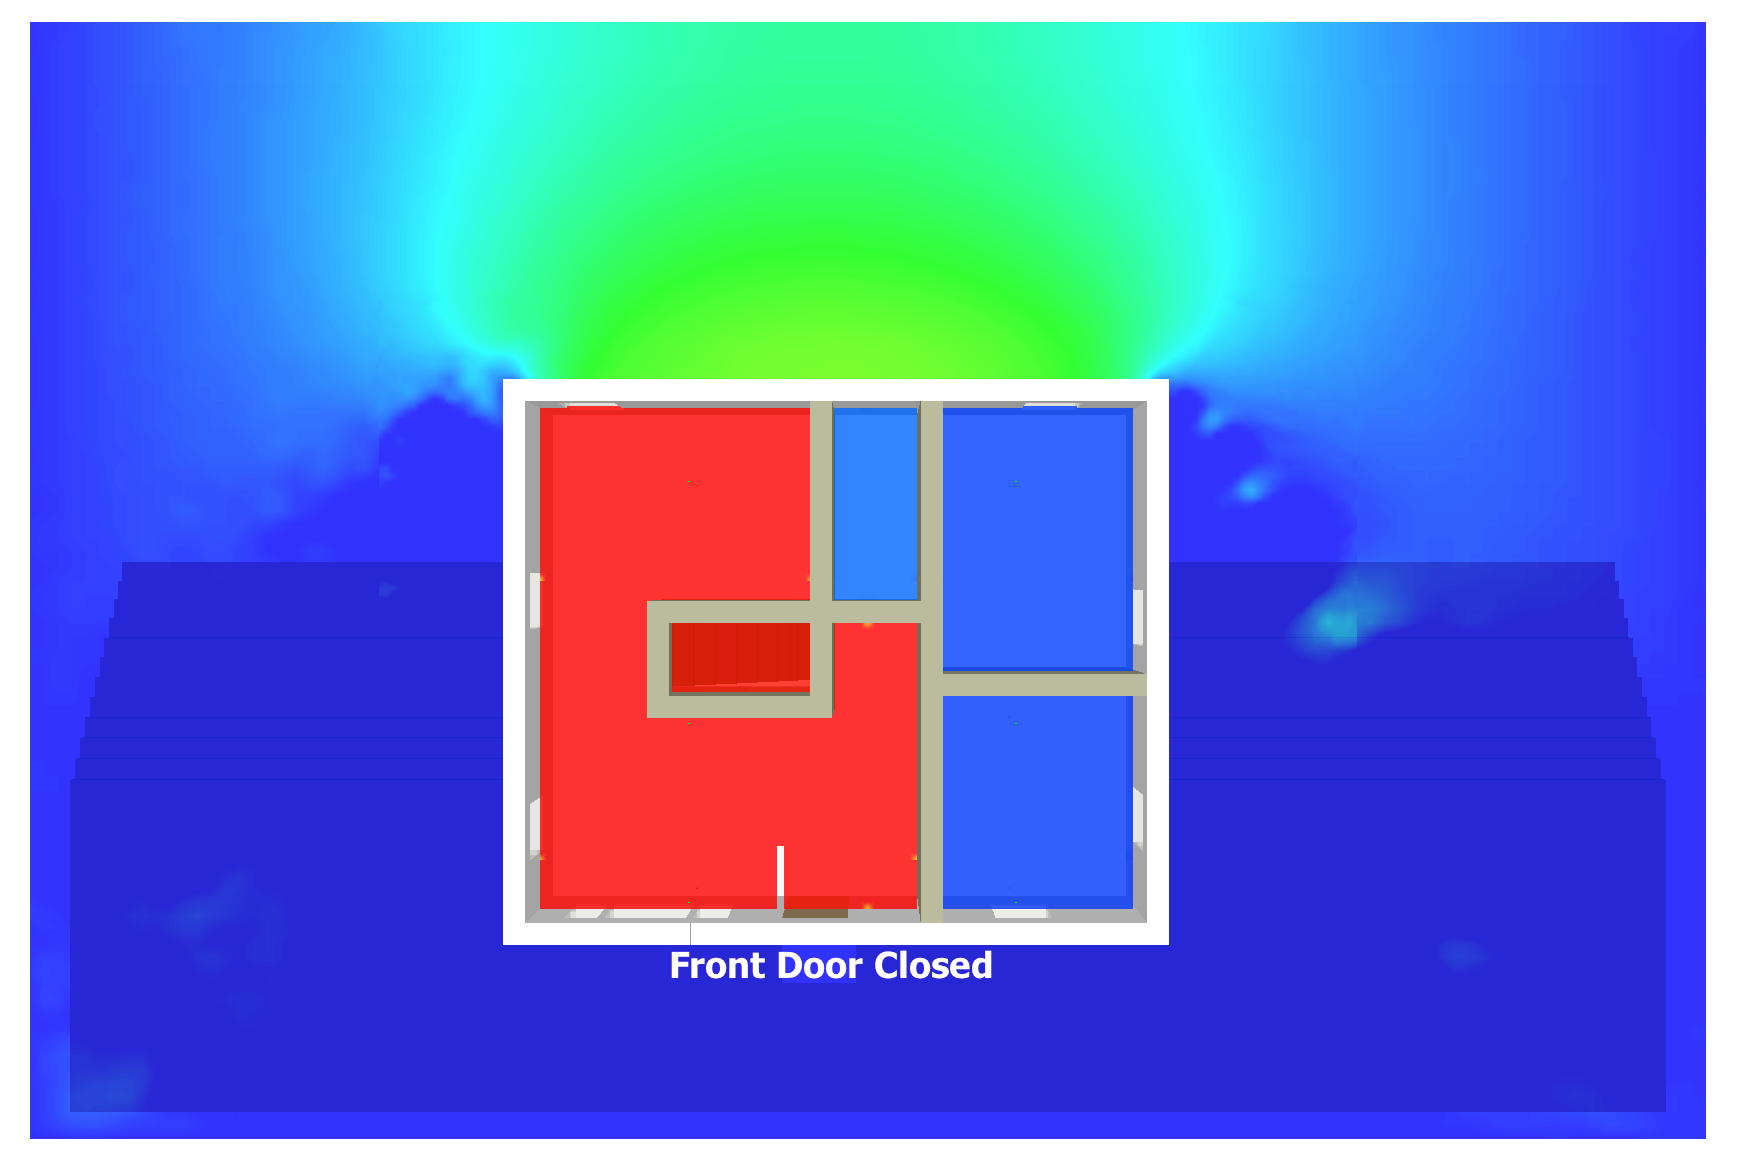
\includegraphics[trim = 1in 1in 1in 1in, clip=true, width=.55\textwidth]{../Figures/pressure_slice_99s}
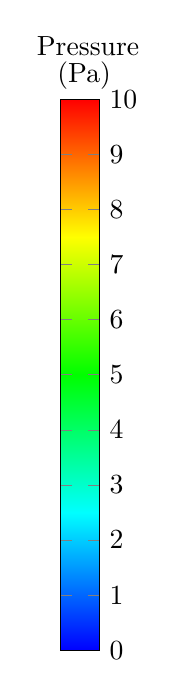
\begin{tikzpicture}
\pgfkeys{/pgf/number format/set thousands separator = {}}
\node at (0.65,0.67) {Pressure};
\node at (0.6,0.3) {(Pa)};
\begin{axis}[
    hide axis,
    scale only axis,
    height=0pt,
    width=0pt,
    colorbar,
    point meta min=0,
    point meta max=10,
    colorbar style={
        height=7cm,
        ytick={0,1,2,...,10}}
    ]
    \addplot [draw=none] coordinates {(0,0)};
\end{axis}
\end{tikzpicture}
 \\
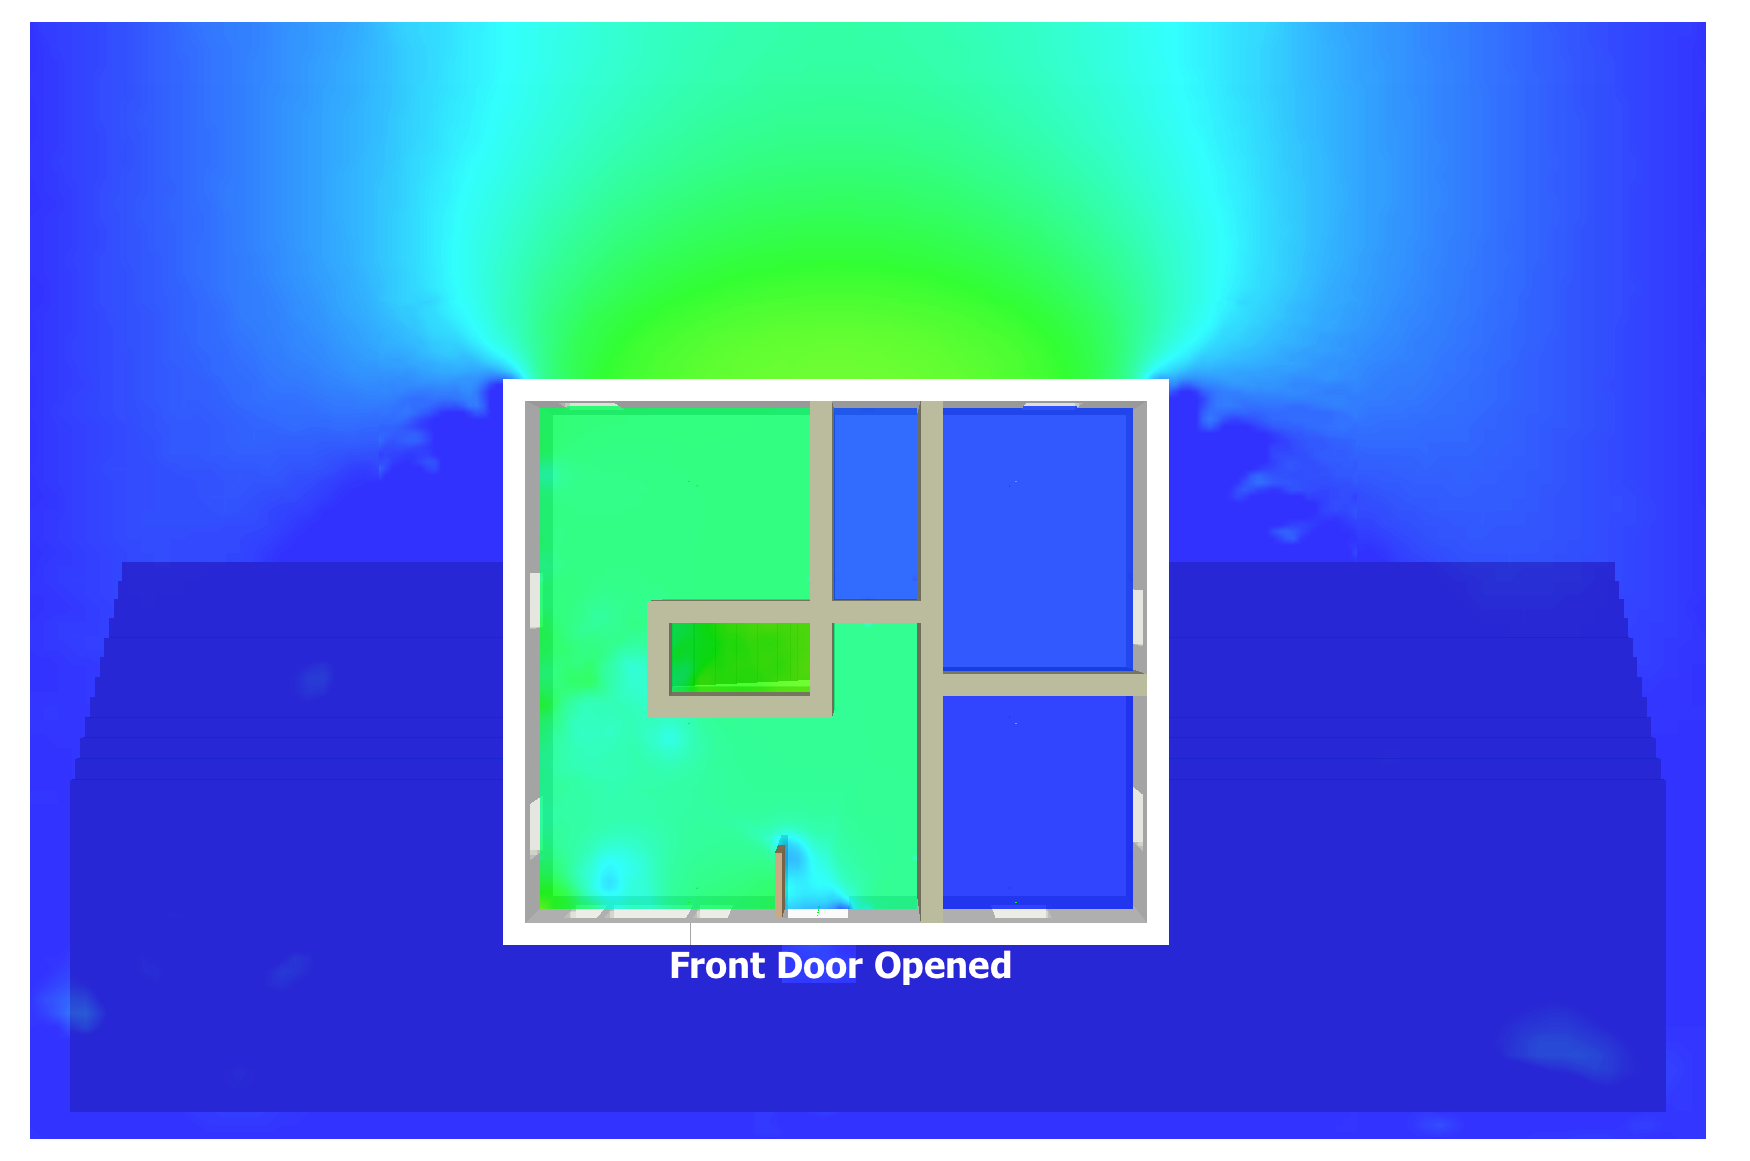
\includegraphics[trim = 1in 1in 1in 1in, clip=true, width=.55\textwidth]{../Figures/pressure_slice_101s}
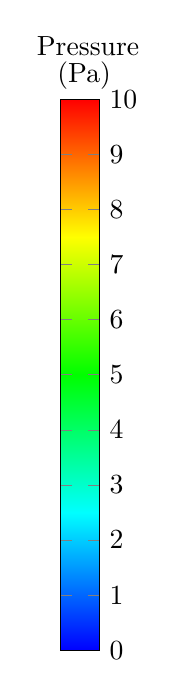
\begin{tikzpicture}
\pgfkeys{/pgf/number format/set thousands separator = {}}
\node at (0.65,0.67) {Pressure};
\node at (0.6,0.3) {(Pa)};
\begin{axis}[
    hide axis,
    scale only axis,
    height=0pt,
    width=0pt,
    colorbar,
    point meta min=0,
    point meta max=10,
    colorbar style={
        height=7cm,
        ytick={0,1,2,...,10}}
    ]
    \addplot [draw=none] coordinates {(0,0)};
\end{axis}
\end{tikzpicture}

\caption[Calculated pressure on first floor 1~s before and after front door opens]
{Calculated pressure contours on first floor of the structure 1~s prior to (top) and 1~s after (bottom) firefighter entry through front door 0.91~m (3~ft) above the floor.}
\label{fig:pressure_slices}
\end{figure}

\clearpage

\section{Velocity}
\label{velocity}

Gases flow from a region of high pressure towards a region of lower pressure. Once the front door opened, the gases in the basement at an elevated temperature and pressure flowed upward into the interior stairwell and exited the structure via the front door. The velocity contours shown in Fig.~\ref{fig:velocity_slices} indicate the magnitude of flow velocities within the structure before and after the front door is opened.

In Fig.~\ref{fig:velocity_slices}, the velocity profile within the high-hazard area (first floor) is shown via two snapshots in time to illustrate the change in the interior conditions 0.91~m (3~ft) above the floor. The first snapshot is shown at a simulation time of 99~s, which is 1~s before the front door is opened, and the second snapshot is shown at a simulation time of 101~s, which is 1~s after the front door is opened. The velocity contours shown indicate that prior to the front door being opened, there is minimal flow on the first floor. However, after the front door is opened a flow path is established allowing the combustion products from the basement fire to flow to the first floor through the interior stairwell. The simulation calculated the flow to exit the structure at approximately 11~m/s (25~mph).

\begin{figure}[!ht]
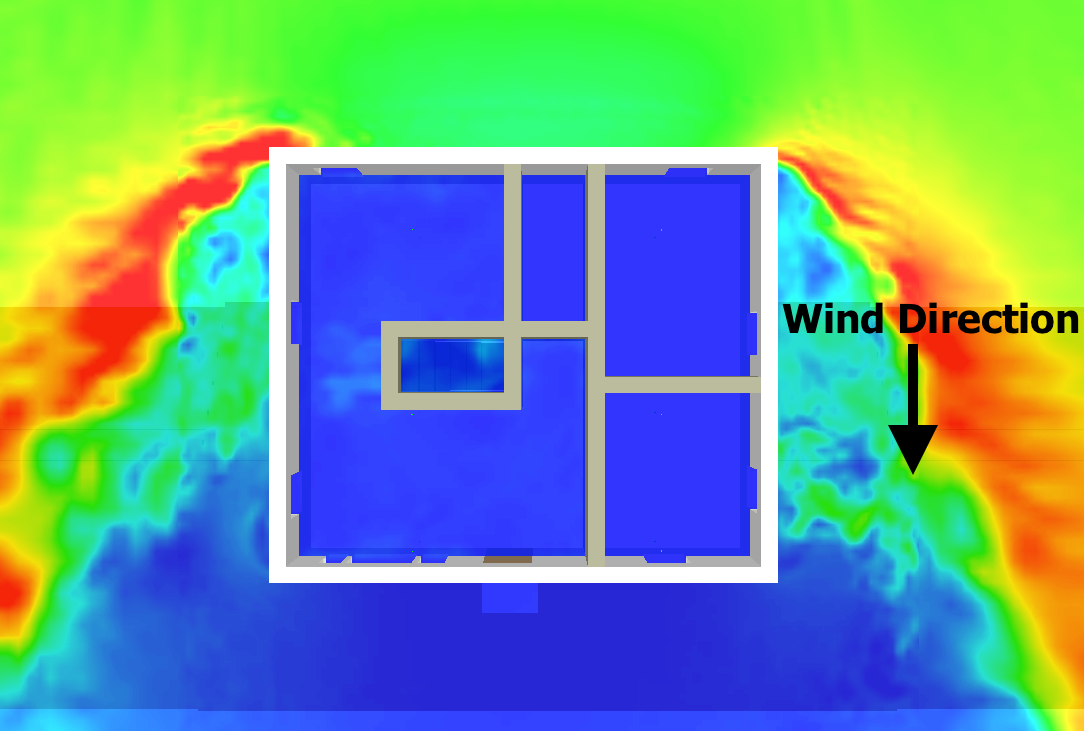
\includegraphics[trim = 0in 1in 0in 1in, clip=true, width=.65\textwidth]{../Figures/velocity_slice_99s}
%\documentclass{standalone}
%\usepackage{pgfplots}
%\begin{document}
%\pgfplotsset{
%	colormap={blackwhite}{[5pt]
%		rgb255(0pt)=(0,0,255); 
%		rgb255(100pt)=(0,255,255); 
%		rgb255(200pt)=(0,255,0); 
%		rgb255(300pt)=(255,255,0); 
%		rgb255(400pt)=(255,0,0)
%	},
%}
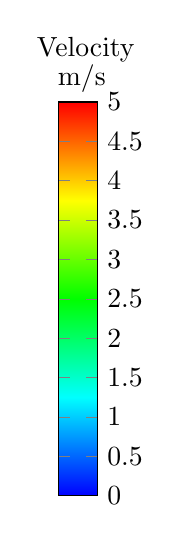
\begin{tikzpicture}
\node at (0.65,0.67) {Velocity};
\node at (0.6,0.3) {m/s};
\begin{axis}[
    hide axis,
    scale only axis,
    height=0pt,
    width=0pt,
    colorbar,
    point meta min=0,
    point meta max=5,
    colorbar style={
        height=5cm,
        ytick={0,0.5,1,...,5}
    }]
    \addplot [draw=none] coordinates {(0,0)};
\end{axis}
\end{tikzpicture}
%\end{document}

%\documentclass{standalone}
%\usepackage{pgfplots}
%\begin{document}
%\pgfplotsset{
%	colormap={blackwhite}{[5pt]
%		rgb255(0pt)=(0,0,255); 
%		rgb255(100pt)=(0,255,255); 
%		rgb255(200pt)=(0,255,0); 
%		rgb255(300pt)=(255,255,0); 
%		rgb255(400pt)=(255,0,0)
%	},
%}
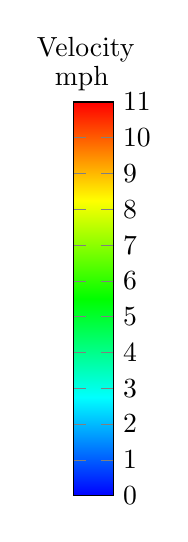
\begin{tikzpicture}
\node at (0.45,0.67) {Velocity};
\node at (0.4,0.3) {mph};
\begin{axis}[
    hide axis,
    scale only axis,
    height=0pt,
    width=0pt,
    colorbar,
    point meta min=0,
    point meta max=11,
    colorbar style={
        height=5cm,
        ytick={0,1,2,...,11}
    }]
    \addplot [draw=none] coordinates {(0,0)};
\end{axis}
\end{tikzpicture}
%\end{document} \\
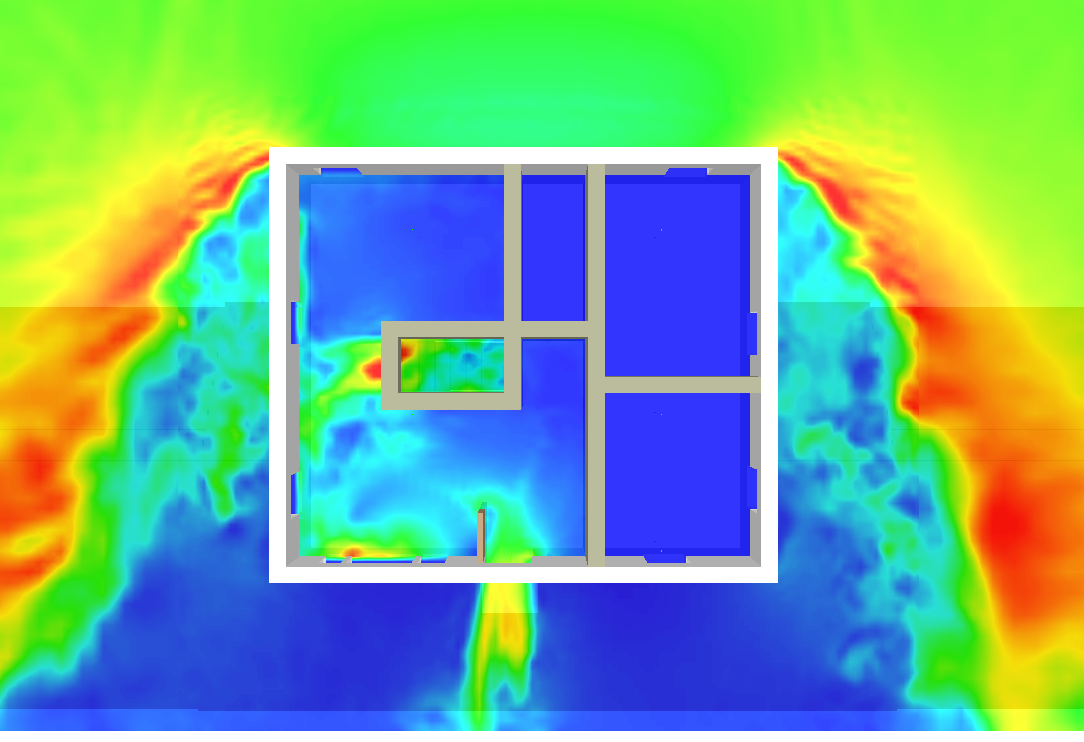
\includegraphics[trim = 0in 1in 0in 1in, clip=true, width=.65\textwidth]{../Figures/velocity_slice_101s}
%\documentclass{standalone}
%\usepackage{pgfplots}
%\begin{document}
%\pgfplotsset{
%	colormap={blackwhite}{[5pt]
%		rgb255(0pt)=(0,0,255); 
%		rgb255(100pt)=(0,255,255); 
%		rgb255(200pt)=(0,255,0); 
%		rgb255(300pt)=(255,255,0); 
%		rgb255(400pt)=(255,0,0)
%	},
%}
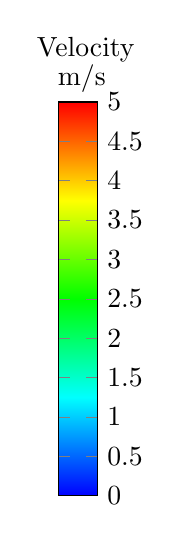
\begin{tikzpicture}
\node at (0.65,0.67) {Velocity};
\node at (0.6,0.3) {m/s};
\begin{axis}[
    hide axis,
    scale only axis,
    height=0pt,
    width=0pt,
    colorbar,
    point meta min=0,
    point meta max=5,
    colorbar style={
        height=5cm,
        ytick={0,0.5,1,...,5}
    }]
    \addplot [draw=none] coordinates {(0,0)};
\end{axis}
\end{tikzpicture}
%\end{document}

%\documentclass{standalone}
%\usepackage{pgfplots}
%\begin{document}
%\pgfplotsset{
%	colormap={blackwhite}{[5pt]
%		rgb255(0pt)=(0,0,255); 
%		rgb255(100pt)=(0,255,255); 
%		rgb255(200pt)=(0,255,0); 
%		rgb255(300pt)=(255,255,0); 
%		rgb255(400pt)=(255,0,0)
%	},
%}
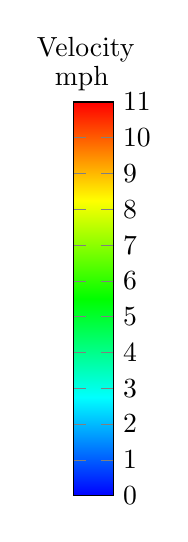
\begin{tikzpicture}
\node at (0.45,0.67) {Velocity};
\node at (0.4,0.3) {mph};
\begin{axis}[
    hide axis,
    scale only axis,
    height=0pt,
    width=0pt,
    colorbar,
    point meta min=0,
    point meta max=11,
    colorbar style={
        height=5cm,
        ytick={0,1,2,...,11}
    }]
    \addplot [draw=none] coordinates {(0,0)};
\end{axis}
\end{tikzpicture}
%\end{document}
\caption[Calculated velocity on first floor 1~s before and after front door opens]
{Calculated velocity contours on first floor of the structure 1~s prior to (top) and 1~s after (bottom) firefighter entry through front door 0.91~m (3~ft) above the floor.}
\label{fig:velocity_slices}
\end{figure}

\clearpage

\section{Temperature}
\label{temp}

Analysis of the temperatures from the simulation focuses on the high-hazard area of the structure: the first floor area between the front door and the top of the interior stairwell. The temperature contours shown in Fig.~\ref{fig:temperature_slice_99s} indicate the gas temperatures within the structure 1~s before the front door was opened 0.91~m (3~ft) above the floor. The overlaid arrows represent the gas flow: the length of the lines represents speeds and the direction of the arrow represents the flow direction. Prior to the door opening, the open living area and kitchen on the first floor were approximately 60~$^{\circ}$C (140~$^{\circ}$F) while the peak temperatures were concentrated near the interior stairwell, 105~$^{\circ}$C (220~$^{\circ}$F). Note that there is very minimal flow throughout the first floor. Figures~\ref{fig:temperature_slice_101s} and \ref{fig:temperature_slice_105s} show gas temperature contours at 0.91~m (3~ft) above the floor, 1~s and 5~s after the front door was opened.

\begin{figure}[!ht]
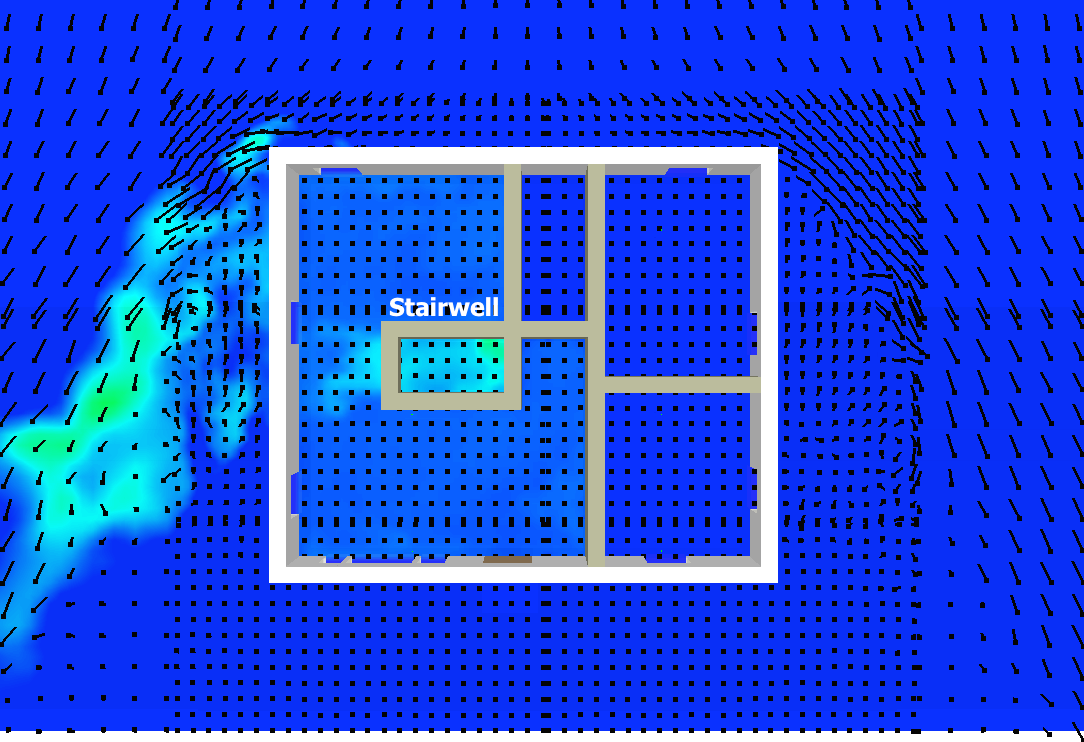
\includegraphics[trim = 1in 1in 1in 1in, clip=true, width=.65\textwidth]{../Figures/temperature_slice_99s}
%\documentclass{standalone}
%\usepackage{pgfplots}
%\begin{document}
%\pgfplotsset{
%	colormap={blackwhite}{[5pt]
%		rgb255(0pt)=(0,0,255); 
%		rgb255(100pt)=(0,255,255); 
%		rgb255(200pt)=(0,255,0); 
%		rgb255(300pt)=(255,255,0); 
%		rgb255(400pt)=(255,0,0)
%	},
%}
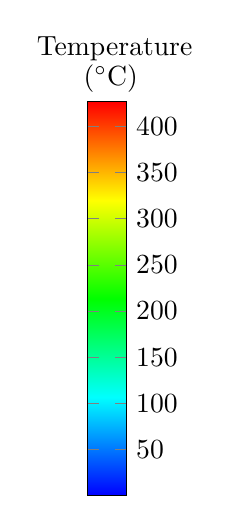
\begin{tikzpicture}
\node at (0.65,0.67) {Temperature};
\node at (0.6,0.3) {($^\circ$C)};
\begin{axis}[
    hide axis,
    scale only axis,
    height=0pt,
    width=0pt,
    colorbar,
    point meta min=0,
    point meta max=426.667,
    colorbar style={
        height=5cm,
        ytick={50,100,...,450}
    }]
    \addplot [draw=none] coordinates {(0,0)};
\end{axis}
\end{tikzpicture}
%\end{document}

%\documentclass{standalone}
%\usepackage{pgfplots}
%\begin{document}
%\pgfplotsset{
%	colormap={blackwhite}{[5pt]
%		rgb255(0pt)=(0,0,255); 
%		rgb255(100pt)=(0,255,255); 
%		rgb255(200pt)=(0,255,0); 
%		rgb255(300pt)=(255,255,0); 
%		rgb255(400pt)=(255,0,0)
%	},
%}
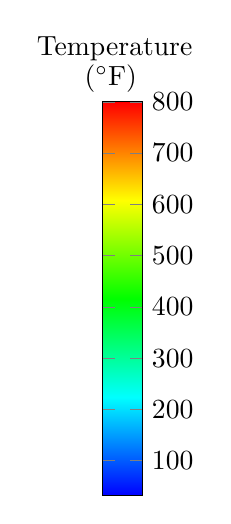
\begin{tikzpicture}
\node at (0.45,0.67) {Temperature};
\node at (0.4,0.3) {($^\circ$F)};
\begin{axis}[
    hide axis,
    scale only axis,
    height=0pt,
    width=0pt,
    colorbar,
    point meta min=32,
    point meta max=800,
    colorbar style={
        height=5cm,
        ytick={100,200,...,800}
    }]
    \addplot [draw=none] coordinates {(0,0)};
\end{axis}
\end{tikzpicture}
%\end{document}
\caption[Calculated temperature on first floor 1~s before front door opened]
{Calculated temperature contours on first floor of the structure 1~s prior to firefighter entry through front door 0.91~m (3~ft) above the floor.}
\label{fig:temperature_slice_99s}
\end{figure}

After the front door is opened, hot fire gases from the basement begin to flow through the interior stairwell into the first floor. Figure~\ref{fig:temperature_slice_101s}, 1~s after the front door was opened, shows that the temperature contours at the top of the stairwell have increased to approximately 200~$^{\circ}$C (392~$^{\circ}$F) with a hot spot that approaches 425~$^{\circ}$C (800~$^{\circ}$F). Figure~\ref{fig:temperature_slice_105s}, 5~s after the front door was opened, shows more significant increases in temperature. The area of at the top of the stairs is most between 375~$^{\circ}$C (700~$^{\circ}$F) and 425~$^{\circ}$C (800~$^{\circ}$F). The gas temperatures 0.91~m (3~ft) above the floor at the front door have also increased to approximately 230~$^{\circ}$C (450~$^{\circ}$F) and show increased flow velocities.

\begin{figure}[!ht]
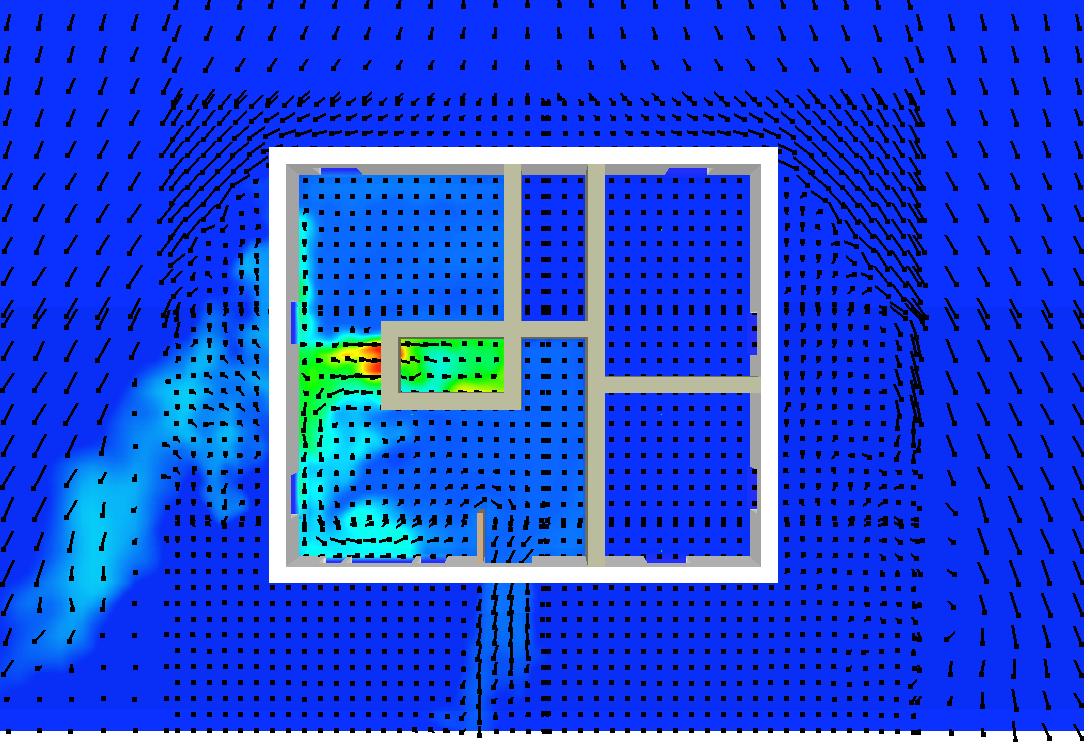
\includegraphics[trim = 1in 1in 1in 1in, clip=true, width=.65\textwidth]{../Figures/temperature_slice_101s}
%\documentclass{standalone}
%\usepackage{pgfplots}
%\begin{document}
%\pgfplotsset{
%	colormap={blackwhite}{[5pt]
%		rgb255(0pt)=(0,0,255); 
%		rgb255(100pt)=(0,255,255); 
%		rgb255(200pt)=(0,255,0); 
%		rgb255(300pt)=(255,255,0); 
%		rgb255(400pt)=(255,0,0)
%	},
%}
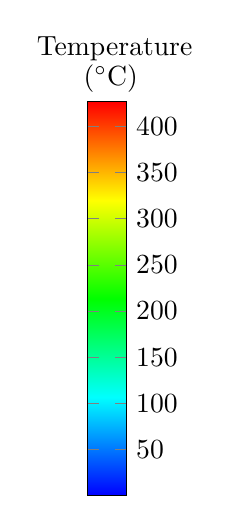
\begin{tikzpicture}
\node at (0.65,0.67) {Temperature};
\node at (0.6,0.3) {($^\circ$C)};
\begin{axis}[
    hide axis,
    scale only axis,
    height=0pt,
    width=0pt,
    colorbar,
    point meta min=0,
    point meta max=426.667,
    colorbar style={
        height=5cm,
        ytick={50,100,...,450}
    }]
    \addplot [draw=none] coordinates {(0,0)};
\end{axis}
\end{tikzpicture}
%\end{document}

%\documentclass{standalone}
%\usepackage{pgfplots}
%\begin{document}
%\pgfplotsset{
%	colormap={blackwhite}{[5pt]
%		rgb255(0pt)=(0,0,255); 
%		rgb255(100pt)=(0,255,255); 
%		rgb255(200pt)=(0,255,0); 
%		rgb255(300pt)=(255,255,0); 
%		rgb255(400pt)=(255,0,0)
%	},
%}
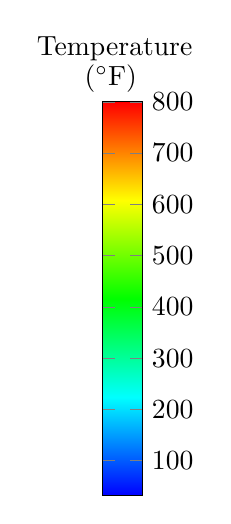
\begin{tikzpicture}
\node at (0.45,0.67) {Temperature};
\node at (0.4,0.3) {($^\circ$F)};
\begin{axis}[
    hide axis,
    scale only axis,
    height=0pt,
    width=0pt,
    colorbar,
    point meta min=32,
    point meta max=800,
    colorbar style={
        height=5cm,
        ytick={100,200,...,800}
    }]
    \addplot [draw=none] coordinates {(0,0)};
\end{axis}
\end{tikzpicture}
%\end{document}
\caption[Calculated temperature on first floor 1~s after front door opens]
{Calculated temperature contours on first floor of the structure 1~s after firefighter entry through front door 0.91~m (3~ft) above the floor.}
\label{fig:temperature_slice_101s}
\end{figure}

\begin{figure}[!ht]
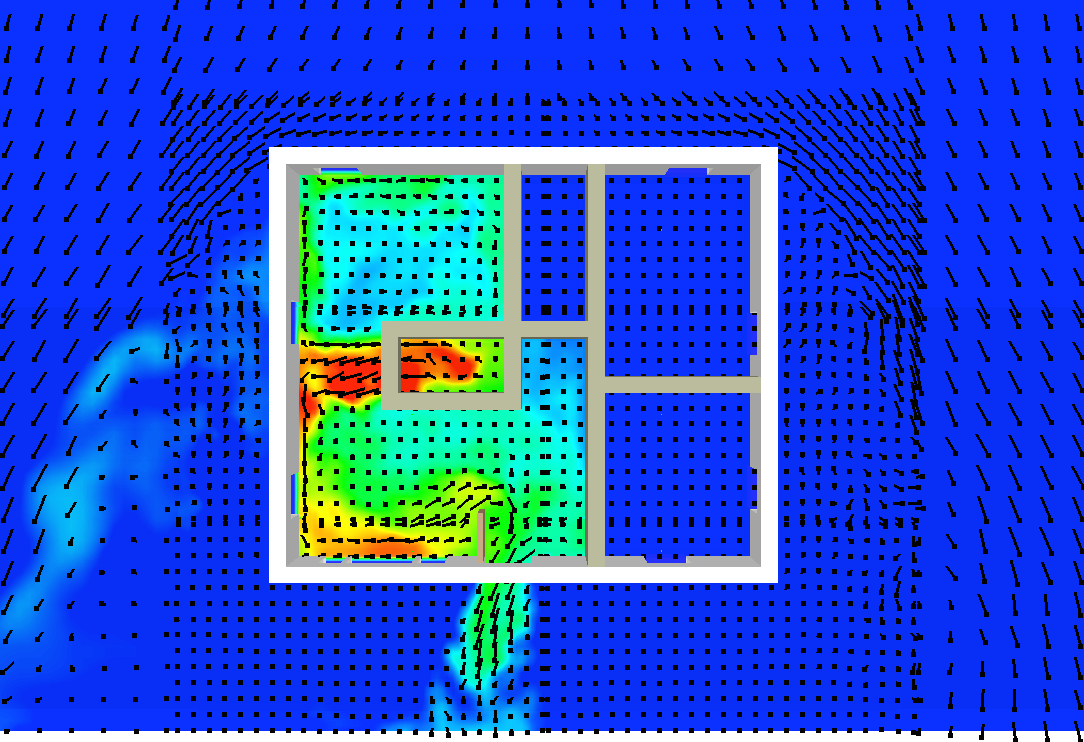
\includegraphics[trim = 1in 1in 1in 1in, clip=true, width=.65\textwidth]{../Figures/temperature_slice_105s}
%\documentclass{standalone}
%\usepackage{pgfplots}
%\begin{document}
%\pgfplotsset{
%	colormap={blackwhite}{[5pt]
%		rgb255(0pt)=(0,0,255); 
%		rgb255(100pt)=(0,255,255); 
%		rgb255(200pt)=(0,255,0); 
%		rgb255(300pt)=(255,255,0); 
%		rgb255(400pt)=(255,0,0)
%	},
%}
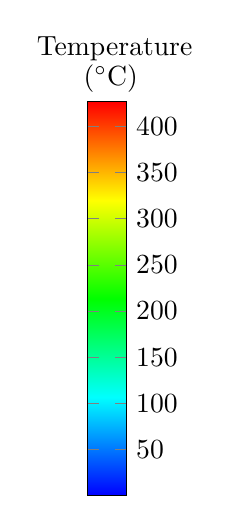
\begin{tikzpicture}
\node at (0.65,0.67) {Temperature};
\node at (0.6,0.3) {($^\circ$C)};
\begin{axis}[
    hide axis,
    scale only axis,
    height=0pt,
    width=0pt,
    colorbar,
    point meta min=0,
    point meta max=426.667,
    colorbar style={
        height=5cm,
        ytick={50,100,...,450}
    }]
    \addplot [draw=none] coordinates {(0,0)};
\end{axis}
\end{tikzpicture}
%\end{document}

%\documentclass{standalone}
%\usepackage{pgfplots}
%\begin{document}
%\pgfplotsset{
%	colormap={blackwhite}{[5pt]
%		rgb255(0pt)=(0,0,255); 
%		rgb255(100pt)=(0,255,255); 
%		rgb255(200pt)=(0,255,0); 
%		rgb255(300pt)=(255,255,0); 
%		rgb255(400pt)=(255,0,0)
%	},
%}
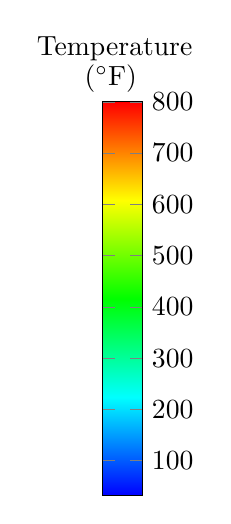
\begin{tikzpicture}
\node at (0.45,0.67) {Temperature};
\node at (0.4,0.3) {($^\circ$F)};
\begin{axis}[
    hide axis,
    scale only axis,
    height=0pt,
    width=0pt,
    colorbar,
    point meta min=32,
    point meta max=800,
    colorbar style={
        height=5cm,
        ytick={100,200,...,800}
    }]
    \addplot [draw=none] coordinates {(0,0)};
\end{axis}
\end{tikzpicture}
%\end{document}
\caption[Calculated temperature on first floor 5~s after front door opens]
{Calculated temperature contours on first floor of the structure 5~s after firefighter entry through front door 0.91~m (3~ft) above the floor.}
\label{fig:temperature_slice_105s}
\end{figure}

\clearpage

\chapter{Discussion}
\label{discuss}
The results of the simulation are discussed in the following sections. Section~\ref{simulated_flow_path} addresses the results of the simulation as they relate to the flow path that was established in the interior stairwell through the front door. Section~\ref{assessing_hazard} examines the model results as they relate to the hazardous conditions and exposure temperatures on the first floor. Section~\ref{tactical_considerations} discusses tactical considerations and outcomes of the fire incident as they relate to the fire dynamics and flow path conditions that have been observed in recent experimental research.

\section{Simulated Flow Path}
\label{simulated_flow_path}

The report from Prince George's County Fire/EMS~\cite{PGCounty2013} indicated that two firefighters from Truck 809 were injured after making entry to the first floor and had to either bail out through a window or be rescued through the front door. From Section~\ref{temp}, the conditions on the first floor were initially tenable. After the front door was opened, however, the simulation results indicate that a high hazard area existed in the first floor that exceeded the conditions of a Class~III exposure (temperatures greater than 260~$^{\circ}$C or 500~$^{\circ}$F)~\cite{Donnelly2006}.

The simulation results indicate that a flow path was established between the open vents (windows and door) on the rear side of the basement and front side of the structure (through the front door of the first floor) after the front door was opened. Strong winds (8.9~m/s (20~mph)) pushed air into the rear side of the basement through window failures and combined with buoyant combustion gases to pressurize the structure. Opening the front door provided a pressure relief; this resulted in a rapid change in the conditions within the structure and the establishment of a flow path. After the front door was opened, the combustion gases at elevated temperature and pressure in the basement flowed towards lower pressure regions outside of the structure on the leeward side (front of structure) via the interior stairwell. The two injured firefighters were located in the flow path on first floor between the top of the interior stairwell and the front door.

To examine the impact of opening the front door on the establishment of a flow path, flow conditions are examined along the centerline of the interior stairwell doorway and at the front door. Figure~\ref{fig:flow_path_99s} shows the flow vectors at the first floor stairwell doorway 1 second before the front door was opened. Note that length and direction of the arrow indicates the magnitude and direction of the flow respectively. The color of the arrow corresponds to the values from the included temperature scales. Therefore, a short blue arrow represents slow moving, cool gas while a long red arrow represents fast moving, high temperature gas. Prior to the door opening, there is minimal flow through the first floor stairwell door and the temperature peak is approximately 125~$^{\circ}$C (257~~$^{\circ}$F) as shown in Figure~\ref{fig:flow_path_99s}. One second after the door opened, Figure~\ref{fig:flow_path_101s}, there is noticeable flow through both the stairwell doorway and through the front door. Simulation temperatures at the stairwell increased to approximately 200~$^{\circ}$C (392~~$^{\circ}$F) and temperatures through the doorway are approximately 100~$^{\circ}$C (212~~$^{\circ}$F). These values are also shown in planar contours 1~m above the floor in Figs.~\ref{fig:velocity_slices} and \ref{fig:temperature_slice_101s} for velocity and temperature, respectively.

\begin{figure}[!ht]
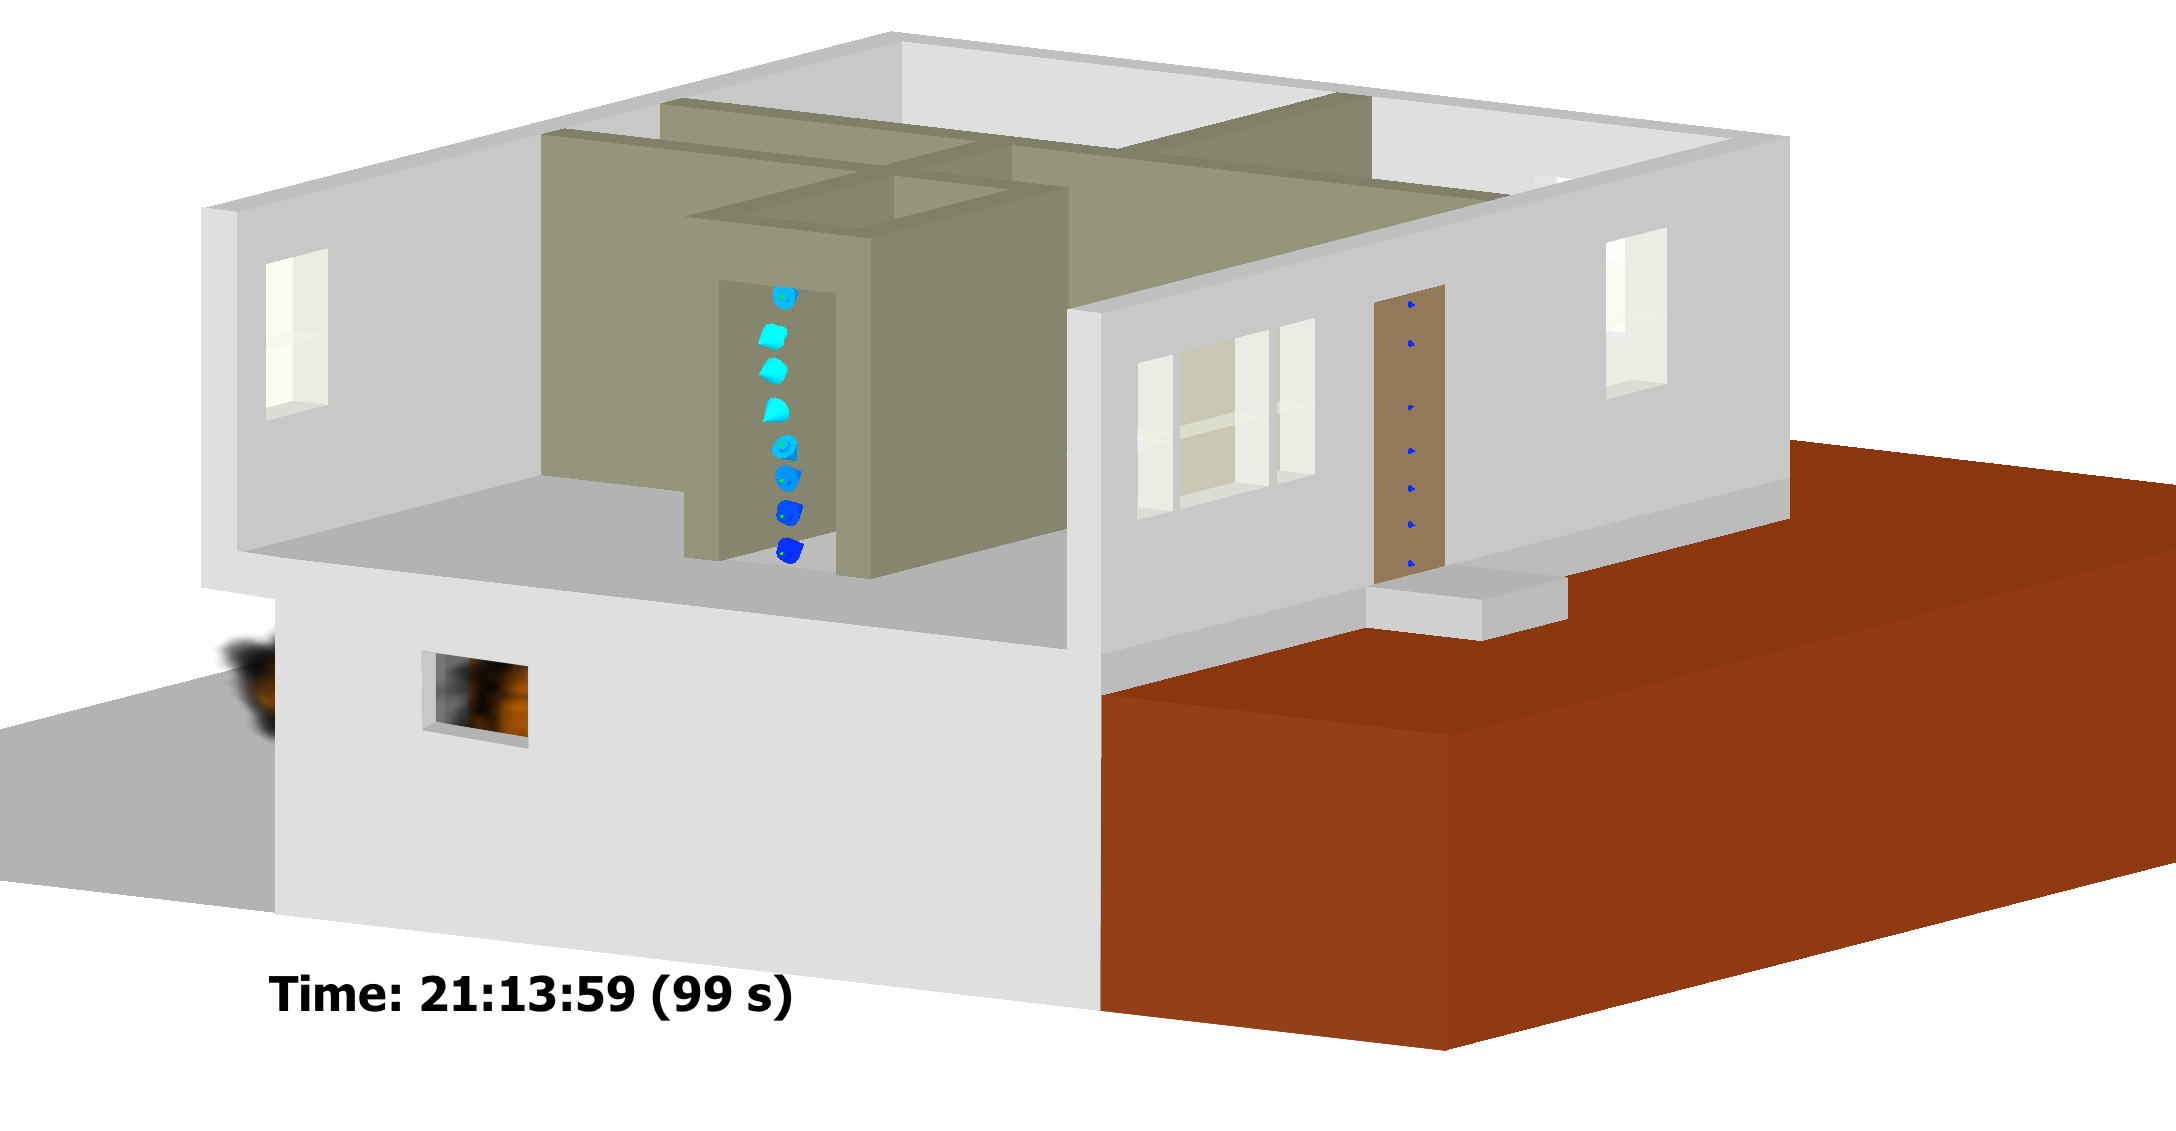
\includegraphics[trim = 2.5in 0in 4in 0in, clip=true, width=.65\textwidth]{../Figures/flow_vector_99s}
%\documentclass{standalone}
%\usepackage{pgfplots}
%\begin{document}
%\pgfplotsset{
%	colormap={blackwhite}{[5pt]
%		rgb255(0pt)=(0,0,255); 
%		rgb255(100pt)=(0,255,255); 
%		rgb255(200pt)=(0,255,0); 
%		rgb255(300pt)=(255,255,0); 
%		rgb255(400pt)=(255,0,0)
%	},
%}
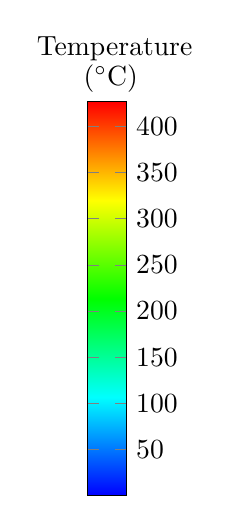
\begin{tikzpicture}
\node at (0.65,0.67) {Temperature};
\node at (0.6,0.3) {($^\circ$C)};
\begin{axis}[
    hide axis,
    scale only axis,
    height=0pt,
    width=0pt,
    colorbar,
    point meta min=0,
    point meta max=426.667,
    colorbar style={
        height=5cm,
        ytick={50,100,...,450}
    }]
    \addplot [draw=none] coordinates {(0,0)};
\end{axis}
\end{tikzpicture}
%\end{document}

%\documentclass{standalone}
%\usepackage{pgfplots}
%\begin{document}
%\pgfplotsset{
%	colormap={blackwhite}{[5pt]
%		rgb255(0pt)=(0,0,255); 
%		rgb255(100pt)=(0,255,255); 
%		rgb255(200pt)=(0,255,0); 
%		rgb255(300pt)=(255,255,0); 
%		rgb255(400pt)=(255,0,0)
%	},
%}
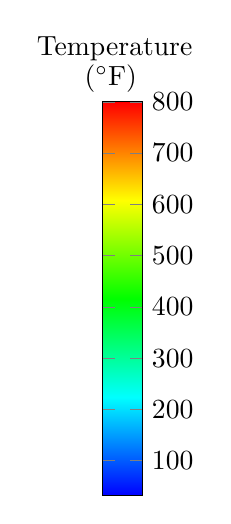
\begin{tikzpicture}
\node at (0.45,0.67) {Temperature};
\node at (0.4,0.3) {($^\circ$F)};
\begin{axis}[
    hide axis,
    scale only axis,
    height=0pt,
    width=0pt,
    colorbar,
    point meta min=32,
    point meta max=800,
    colorbar style={
        height=5cm,
        ytick={100,200,...,800}
    }]
    \addplot [draw=none] coordinates {(0,0)};
\end{axis}
\end{tikzpicture}
%\end{document}
\caption[Flow path vectors at front door and top of stairwell 1~s before front door was opened]
{Flow path vectors at front door and top of stairwell 1~s before front door was opened.}
\label{fig:flow_path_99s}
\end{figure}

\begin{figure}[!ht]
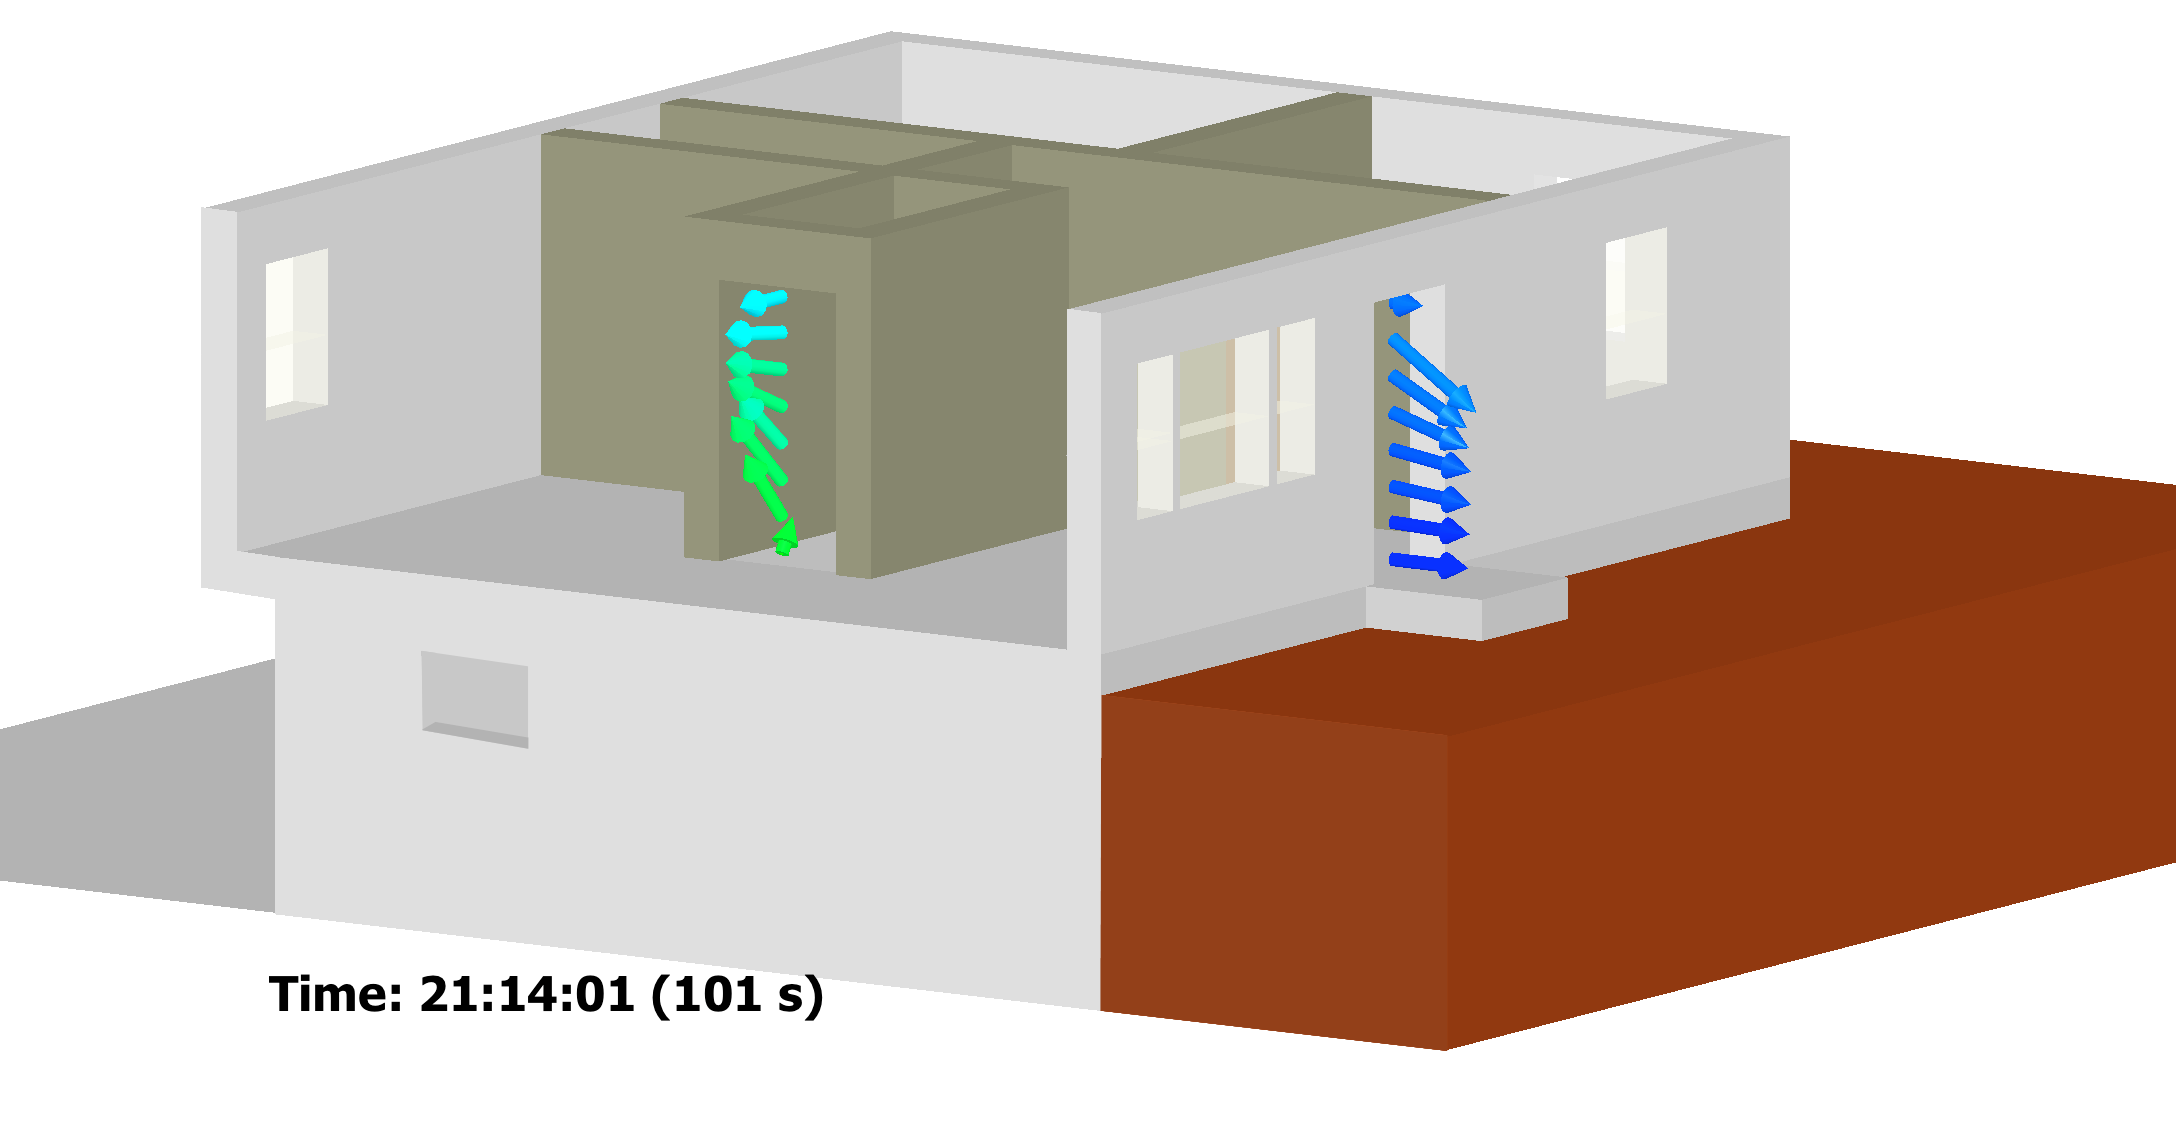
\includegraphics[trim = 2.5in 0in 4in 0in, clip=true, width=.65\textwidth]{../Figures/flow_vector_101s}
%\documentclass{standalone}
%\usepackage{pgfplots}
%\begin{document}
%\pgfplotsset{
%	colormap={blackwhite}{[5pt]
%		rgb255(0pt)=(0,0,255); 
%		rgb255(100pt)=(0,255,255); 
%		rgb255(200pt)=(0,255,0); 
%		rgb255(300pt)=(255,255,0); 
%		rgb255(400pt)=(255,0,0)
%	},
%}
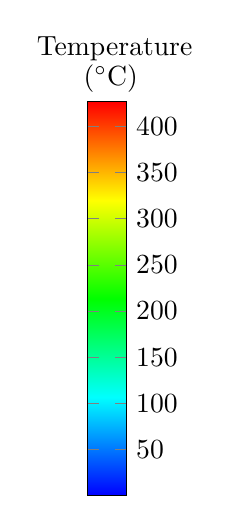
\begin{tikzpicture}
\node at (0.65,0.67) {Temperature};
\node at (0.6,0.3) {($^\circ$C)};
\begin{axis}[
    hide axis,
    scale only axis,
    height=0pt,
    width=0pt,
    colorbar,
    point meta min=0,
    point meta max=426.667,
    colorbar style={
        height=5cm,
        ytick={50,100,...,450}
    }]
    \addplot [draw=none] coordinates {(0,0)};
\end{axis}
\end{tikzpicture}
%\end{document}

%\documentclass{standalone}
%\usepackage{pgfplots}
%\begin{document}
%\pgfplotsset{
%	colormap={blackwhite}{[5pt]
%		rgb255(0pt)=(0,0,255); 
%		rgb255(100pt)=(0,255,255); 
%		rgb255(200pt)=(0,255,0); 
%		rgb255(300pt)=(255,255,0); 
%		rgb255(400pt)=(255,0,0)
%	},
%}
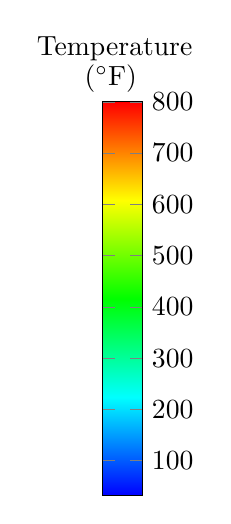
\begin{tikzpicture}
\node at (0.45,0.67) {Temperature};
\node at (0.4,0.3) {($^\circ$F)};
\begin{axis}[
    hide axis,
    scale only axis,
    height=0pt,
    width=0pt,
    colorbar,
    point meta min=32,
    point meta max=800,
    colorbar style={
        height=5cm,
        ytick={100,200,...,800}
    }]
    \addplot [draw=none] coordinates {(0,0)};
\end{axis}
\end{tikzpicture}
%\end{document}
\caption[Flow path vectors at front door and top of stairwell 1~s after front door was opened]
{Flow path vectors at front door and top of stairwell 1~s after front door was opened.}
\label{fig:flow_path_101s} 
\end{figure}

\clearpage

At the estimated time of firefighter entry to the first floor (142~s into the simulation; 21:14:42 according to Table~\ref{tab:combined_timeline}), the simulated flow magnitudes through the first floor (stairwell and front doors) remained similar to the conditions just after opening the front door. Velocities through both the doorway at the top of the stairs and the front door were approximately 13~m/s (29~mph), faster than the incident wind  speed (9~m/s or 20~mph) because of the addition of the bouyancy of the fire plume. The model temperatures increased through the stairwell doorway to between 400~$^{\circ}$C and 425~$^{\circ}$C (750-800~$^{\circ}$F) and through the front door to approximately 375~$^{\circ}$C (700~$^{\circ}$F). From the approximate timeline (Table~\ref{tab:combined_timeline}), the front door was forced closed due to airflow pushing against the front door 207~s into the simulation. Figures~\ref{fig:flow_path_206s} and \ref{fig:flow_path_207s} show the conditions 1~s prior to and after the front door closed. The figures show that while the closed door stopped significant flow through the stairwell door and onto the first floor, temperature hazard for the firefighters (temperatures at or above 400~$^{\circ}$C or 750~$^{\circ}$F) remained.

\begin{figure}[!ht]
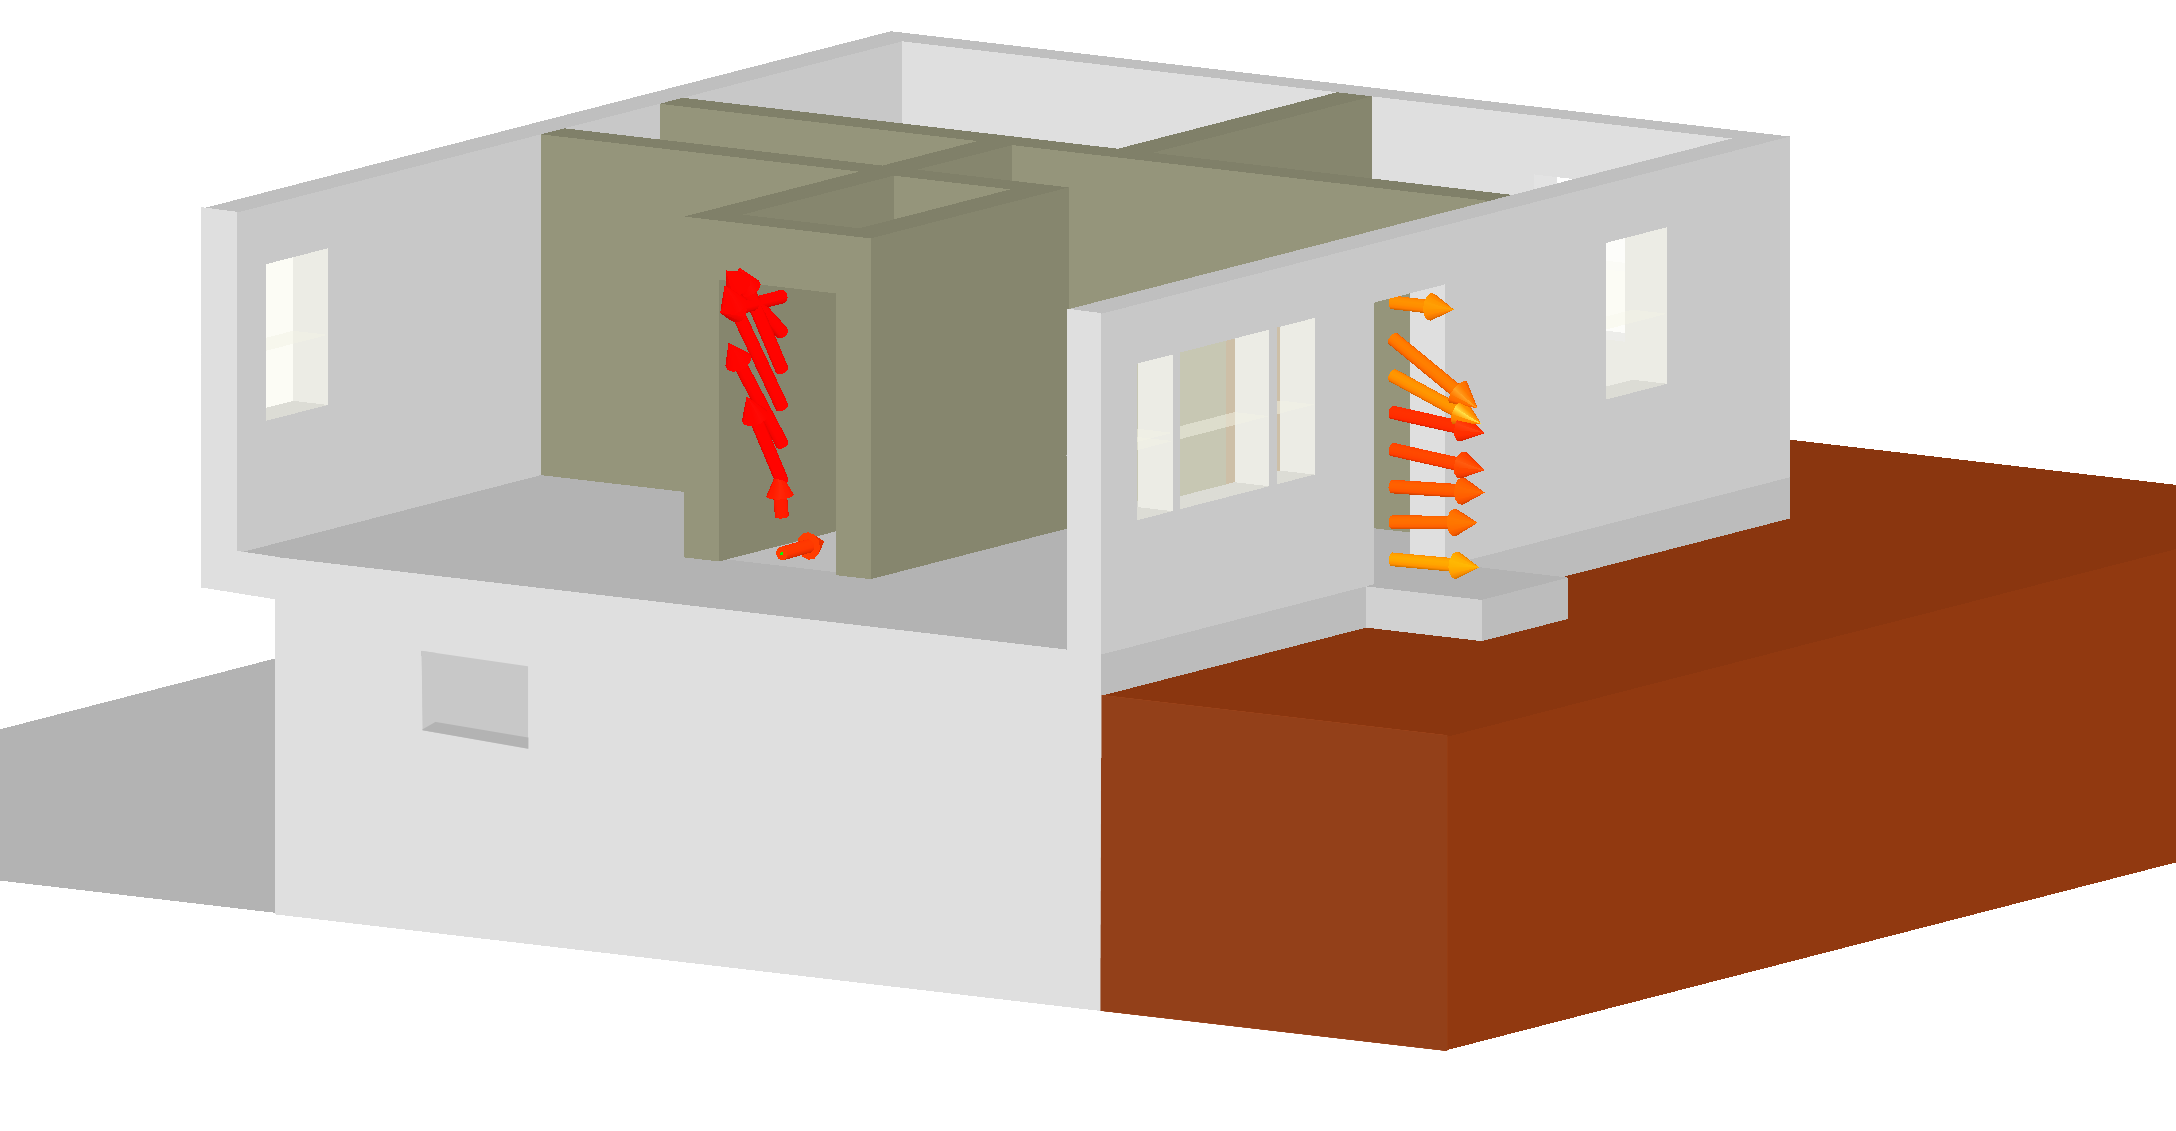
\includegraphics[trim = 2.5in 0in 4in 0in, clip=true, width=.65\textwidth]{../Figures/flow_vector_142s}
%\documentclass{standalone}
%\usepackage{pgfplots}
%\begin{document}
%\pgfplotsset{
%	colormap={blackwhite}{[5pt]
%		rgb255(0pt)=(0,0,255); 
%		rgb255(100pt)=(0,255,255); 
%		rgb255(200pt)=(0,255,0); 
%		rgb255(300pt)=(255,255,0); 
%		rgb255(400pt)=(255,0,0)
%	},
%}
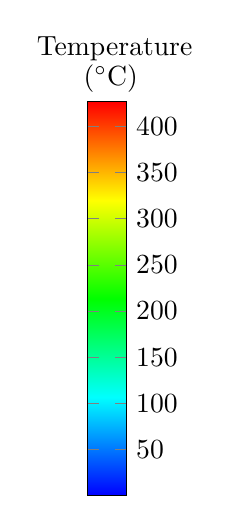
\begin{tikzpicture}
\node at (0.65,0.67) {Temperature};
\node at (0.6,0.3) {($^\circ$C)};
\begin{axis}[
    hide axis,
    scale only axis,
    height=0pt,
    width=0pt,
    colorbar,
    point meta min=0,
    point meta max=426.667,
    colorbar style={
        height=5cm,
        ytick={50,100,...,450}
    }]
    \addplot [draw=none] coordinates {(0,0)};
\end{axis}
\end{tikzpicture}
%\end{document}

%\documentclass{standalone}
%\usepackage{pgfplots}
%\begin{document}
%\pgfplotsset{
%	colormap={blackwhite}{[5pt]
%		rgb255(0pt)=(0,0,255); 
%		rgb255(100pt)=(0,255,255); 
%		rgb255(200pt)=(0,255,0); 
%		rgb255(300pt)=(255,255,0); 
%		rgb255(400pt)=(255,0,0)
%	},
%}
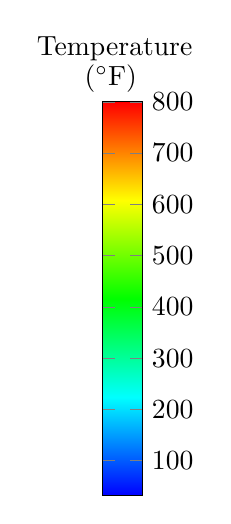
\begin{tikzpicture}
\node at (0.45,0.67) {Temperature};
\node at (0.4,0.3) {($^\circ$F)};
\begin{axis}[
    hide axis,
    scale only axis,
    height=0pt,
    width=0pt,
    colorbar,
    point meta min=32,
    point meta max=800,
    colorbar style={
        height=5cm,
        ytick={100,200,...,800}
    }]
    \addplot [draw=none] coordinates {(0,0)};
\end{axis}
\end{tikzpicture}
%\end{document}
\caption[Flow path vectors at front door and top of stairwell at estimated time of first floor entry]
{Flow path vectors at front door and top of stairwell 42~s after front door was opened, the estimated time of first floor entry.}
\label{fig:flow_path_142s}
\end{figure}

\begin{figure}[!ht]
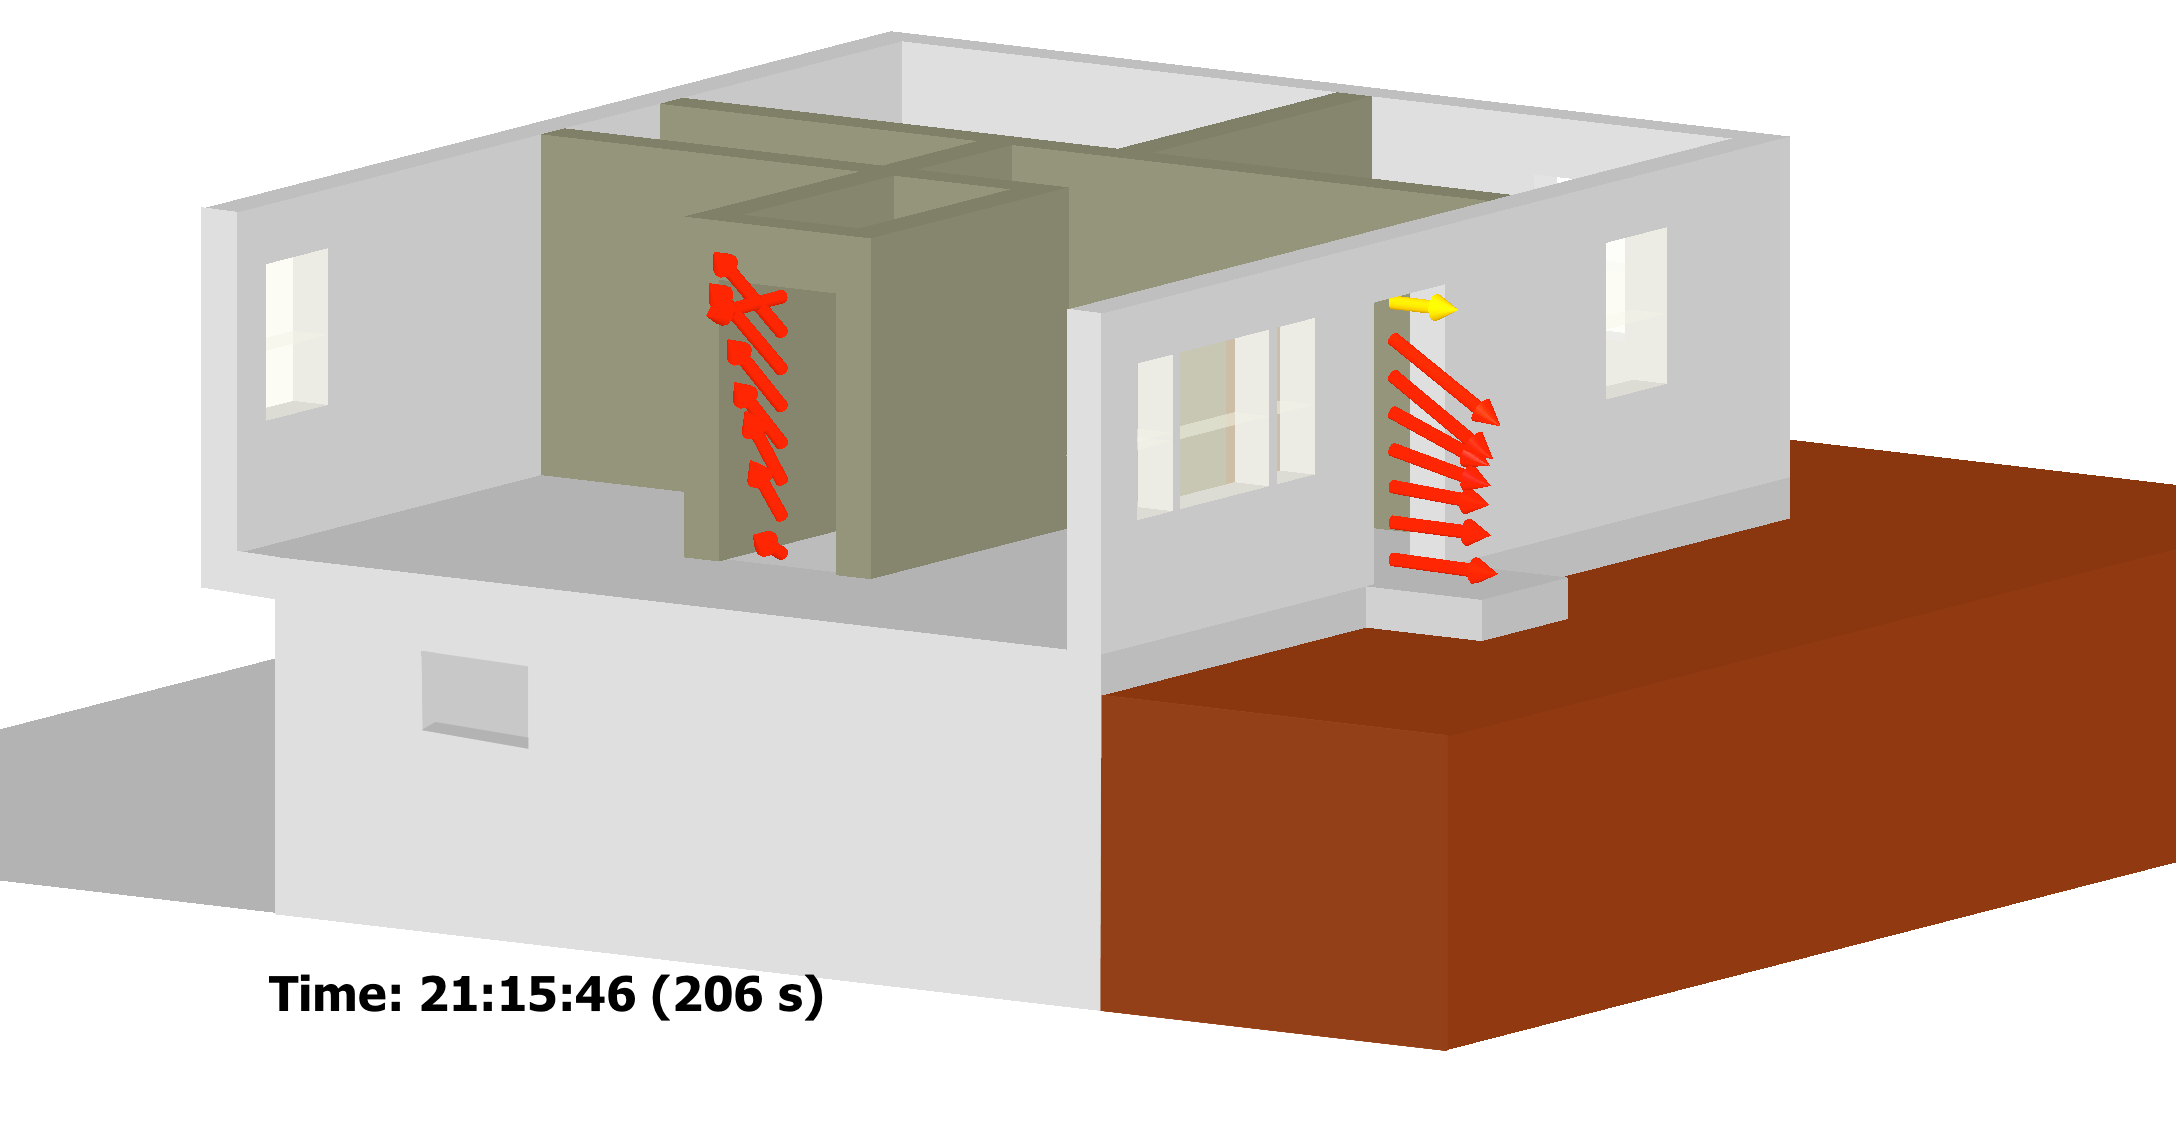
\includegraphics[trim = 2.5in 0in 4in 0in, clip=true, width=.65\textwidth]{../Figures/flow_vector_206s}
%\documentclass{standalone}
%\usepackage{pgfplots}
%\begin{document}
%\pgfplotsset{
%	colormap={blackwhite}{[5pt]
%		rgb255(0pt)=(0,0,255); 
%		rgb255(100pt)=(0,255,255); 
%		rgb255(200pt)=(0,255,0); 
%		rgb255(300pt)=(255,255,0); 
%		rgb255(400pt)=(255,0,0)
%	},
%}
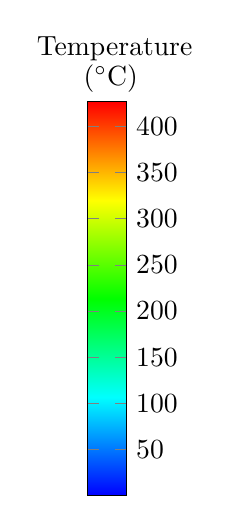
\begin{tikzpicture}
\node at (0.65,0.67) {Temperature};
\node at (0.6,0.3) {($^\circ$C)};
\begin{axis}[
    hide axis,
    scale only axis,
    height=0pt,
    width=0pt,
    colorbar,
    point meta min=0,
    point meta max=426.667,
    colorbar style={
        height=5cm,
        ytick={50,100,...,450}
    }]
    \addplot [draw=none] coordinates {(0,0)};
\end{axis}
\end{tikzpicture}
%\end{document}

%\documentclass{standalone}
%\usepackage{pgfplots}
%\begin{document}
%\pgfplotsset{
%	colormap={blackwhite}{[5pt]
%		rgb255(0pt)=(0,0,255); 
%		rgb255(100pt)=(0,255,255); 
%		rgb255(200pt)=(0,255,0); 
%		rgb255(300pt)=(255,255,0); 
%		rgb255(400pt)=(255,0,0)
%	},
%}
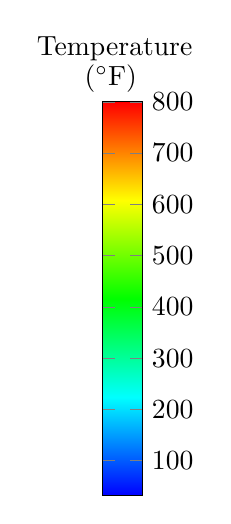
\begin{tikzpicture}
\node at (0.45,0.67) {Temperature};
\node at (0.4,0.3) {($^\circ$F)};
\begin{axis}[
    hide axis,
    scale only axis,
    height=0pt,
    width=0pt,
    colorbar,
    point meta min=32,
    point meta max=800,
    colorbar style={
        height=5cm,
        ytick={100,200,...,800}
    }]
    \addplot [draw=none] coordinates {(0,0)};
\end{axis}
\end{tikzpicture}
%\end{document}
\caption[Flow path vectors at front door and top of stairwell 1~s before front door was closed]
{Flow path vectors at front door and top of stairwell 1~s before front door was closed.}
\label{fig:flow_path_206s}
\end{figure}

\begin{figure}[!ht]
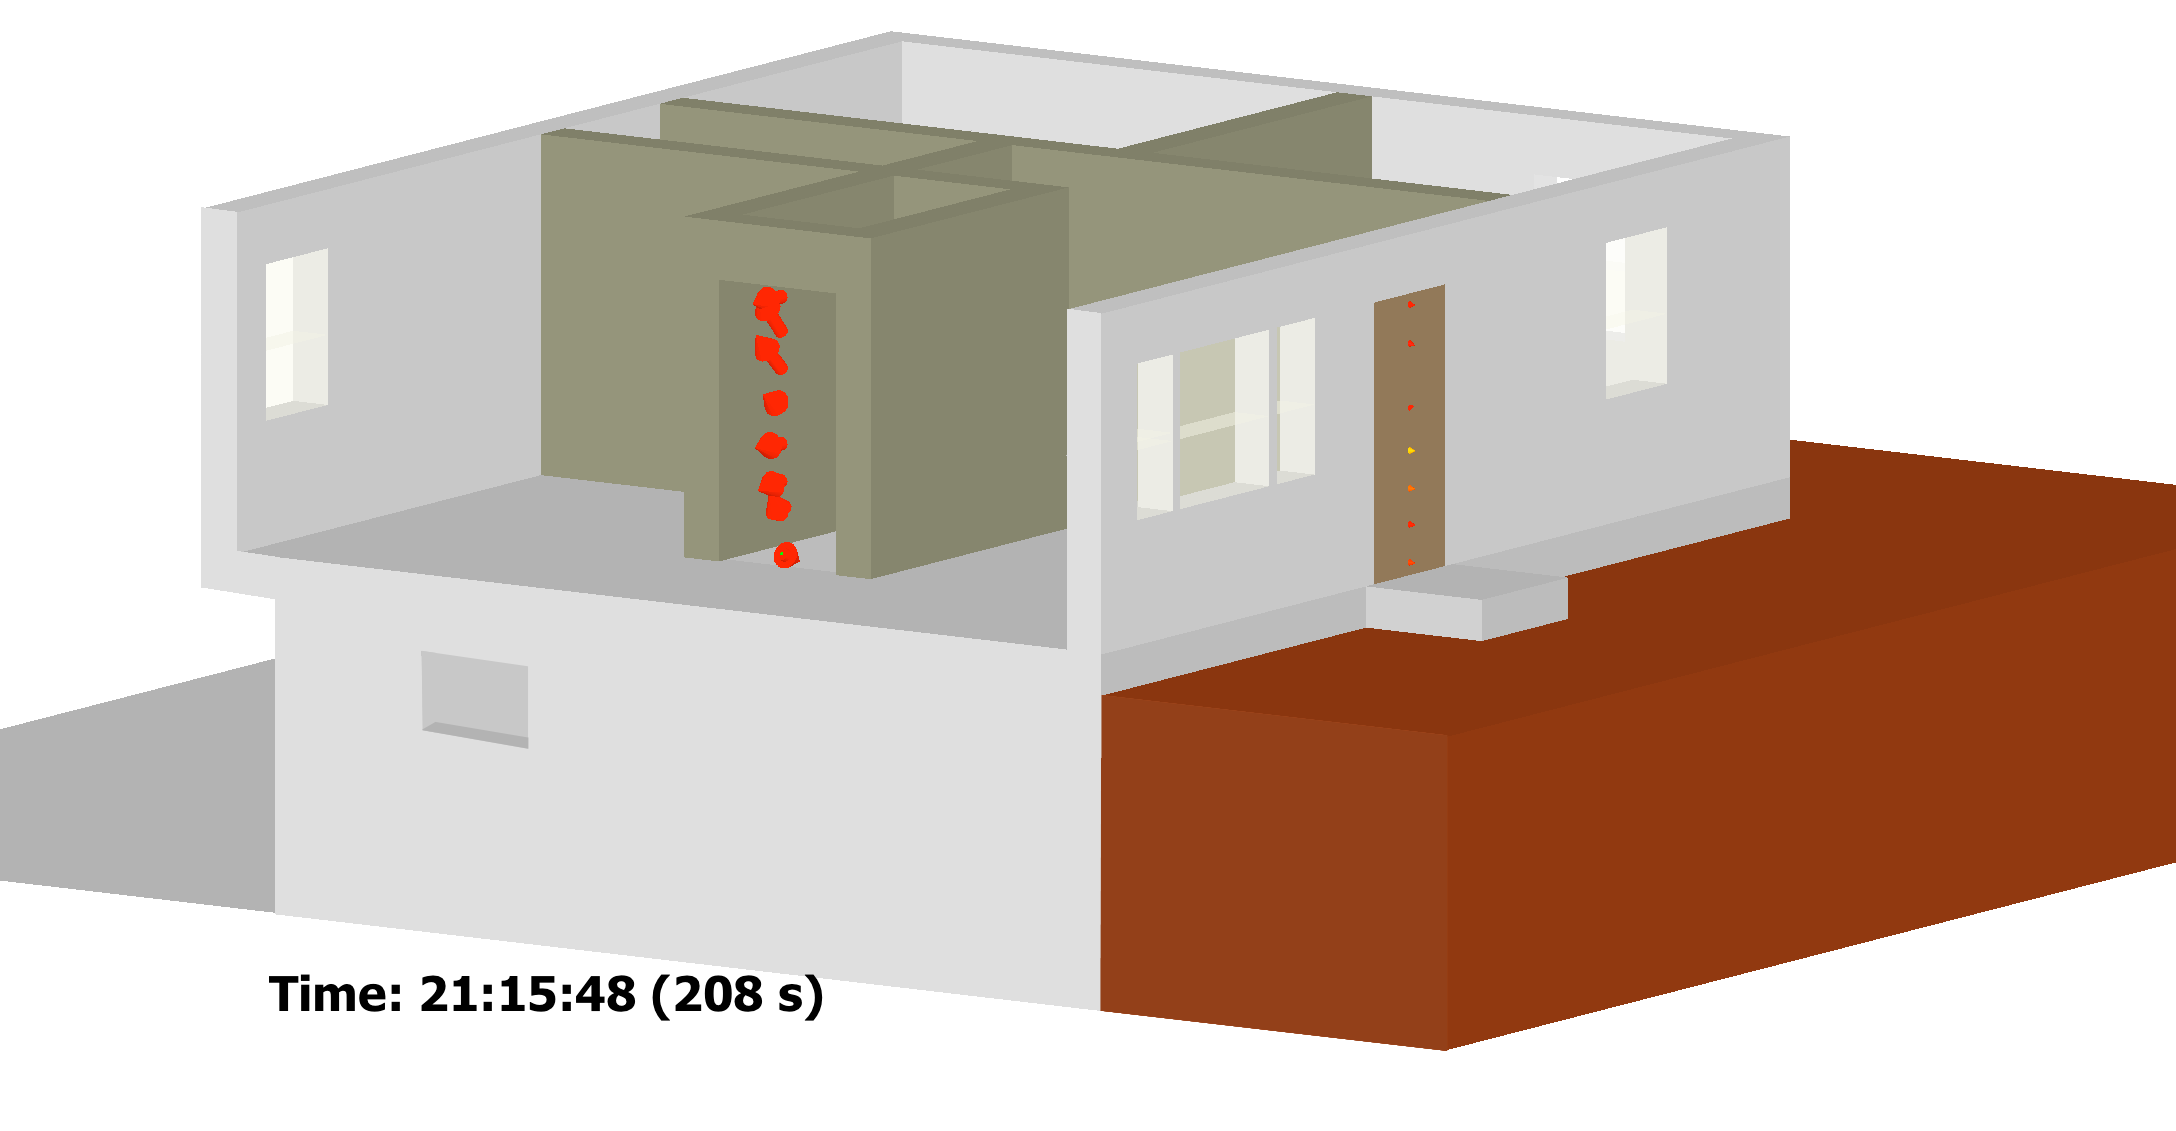
\includegraphics[trim = 2.5in 0in 4in 0in, clip=true, width=.65\textwidth]{../Figures/flow_vector_207s}
%\documentclass{standalone}
%\usepackage{pgfplots}
%\begin{document}
%\pgfplotsset{
%	colormap={blackwhite}{[5pt]
%		rgb255(0pt)=(0,0,255); 
%		rgb255(100pt)=(0,255,255); 
%		rgb255(200pt)=(0,255,0); 
%		rgb255(300pt)=(255,255,0); 
%		rgb255(400pt)=(255,0,0)
%	},
%}
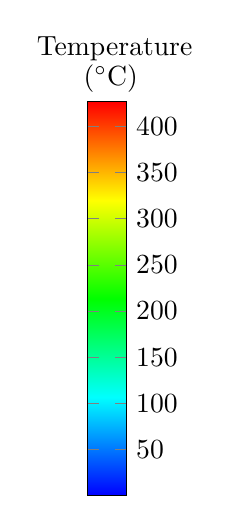
\begin{tikzpicture}
\node at (0.65,0.67) {Temperature};
\node at (0.6,0.3) {($^\circ$C)};
\begin{axis}[
    hide axis,
    scale only axis,
    height=0pt,
    width=0pt,
    colorbar,
    point meta min=0,
    point meta max=426.667,
    colorbar style={
        height=5cm,
        ytick={50,100,...,450}
    }]
    \addplot [draw=none] coordinates {(0,0)};
\end{axis}
\end{tikzpicture}
%\end{document}

%\documentclass{standalone}
%\usepackage{pgfplots}
%\begin{document}
%\pgfplotsset{
%	colormap={blackwhite}{[5pt]
%		rgb255(0pt)=(0,0,255); 
%		rgb255(100pt)=(0,255,255); 
%		rgb255(200pt)=(0,255,0); 
%		rgb255(300pt)=(255,255,0); 
%		rgb255(400pt)=(255,0,0)
%	},
%}
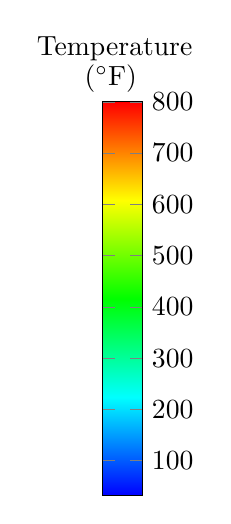
\begin{tikzpicture}
\node at (0.45,0.67) {Temperature};
\node at (0.4,0.3) {($^\circ$F)};
\begin{axis}[
    hide axis,
    scale only axis,
    height=0pt,
    width=0pt,
    colorbar,
    point meta min=32,
    point meta max=800,
    colorbar style={
        height=5cm,
        ytick={100,200,...,800}
    }]
    \addplot [draw=none] coordinates {(0,0)};
\end{axis}
\end{tikzpicture}
%\end{document}
\caption[Flow path vectors at front door and top of stairwell 1~s after front door was closed]
{Flow path vectors at front door and top of stairwell 1~s after front door was closed.}
\label{fig:flow_path_207s}
\end{figure}

\clearpage

\section{Assessing the Hazard}
\label{assessing_hazard}
A person is susceptible to second-degree burn injuries if exposed to temperatures greater than 55~$^{\circ}$C (130~$^{\circ}$F)~\cite{contactburn}. Although firefighters wear protective gear, gear only offers a finite amount of protection. The polycarbonate material in the facepiece of a self-contained breathing apparatus begins to soften when the material temperature reaches approximately 140~$^{\circ}$C (284~$^{\circ}$F)~\cite{mensch2011emergency}. Structural fire fighting coats and pants are tested to withstand temperatures of 260~$^{\circ}$C (500~$^{\circ}$F)~\cite{nfpa2013standard}. Prolonged exposure to elevated temperatures can result in a significant amount of heat transferred to the firefighter, putting him or her at risk. Exposure of equipment to temperatures of 260~$^{\circ}$C (500~$^{\circ}$F) represents a Class~III exposure~\cite{Donnelly2006}. Firefighters are at increased risk levels when encountering Class~III exposure conditions for more than 5~minutes~\cite{Donnelly2006}.

Figures~\ref{fig:int_temp_99s} to \ref{fig:int_temp_142s} show two interior views of temperature contours at particular snapshots in time. The top image is a planar view through the middle of the front door (from the front to the back of the house) which shows the conditions in the living area on the first floor and the conditions in the basement just past the bottom of the stairs. The bottom image shows temperature contours through the middle of the interior stairwell which connected the basement to the first floor of the structure (looking from the rear of the structure towards the front). Prior to the front door being opened (Fig.~\ref{fig:int_temp_99s}, temperatures in excess of 200~$^{\circ}$C (400~$^{\circ}$F) were confined to basement of the structure: specifically the rear of the structure and under the stairwell. One second after the door was opened, hazard in the structure increased within the structure with the most drastic change occurring at the top of the stairwell as peak simulated temperatures exceeded 400~$^{\circ}$C (750~$^{\circ}$F). At the approximate time firefighters made entry to the first floor, Fig.~\ref{fig:int_temp_142s}, the conditions within the flowpath (interior stairwell through front door) had become more severe with temperatures in excess of 400~$^{\circ}$C (750~$^{\circ}$F), which exceeds the Class III exposure of 260~$^{\circ}$C (500~$^{\circ}$F). These high-hazard conditions within the flowpath remained until the model HRR was reduced to simulate the action of applying water the fire. 

\begin{figure}[!ht]
\begin{subfigure}{0.65\textwidth}
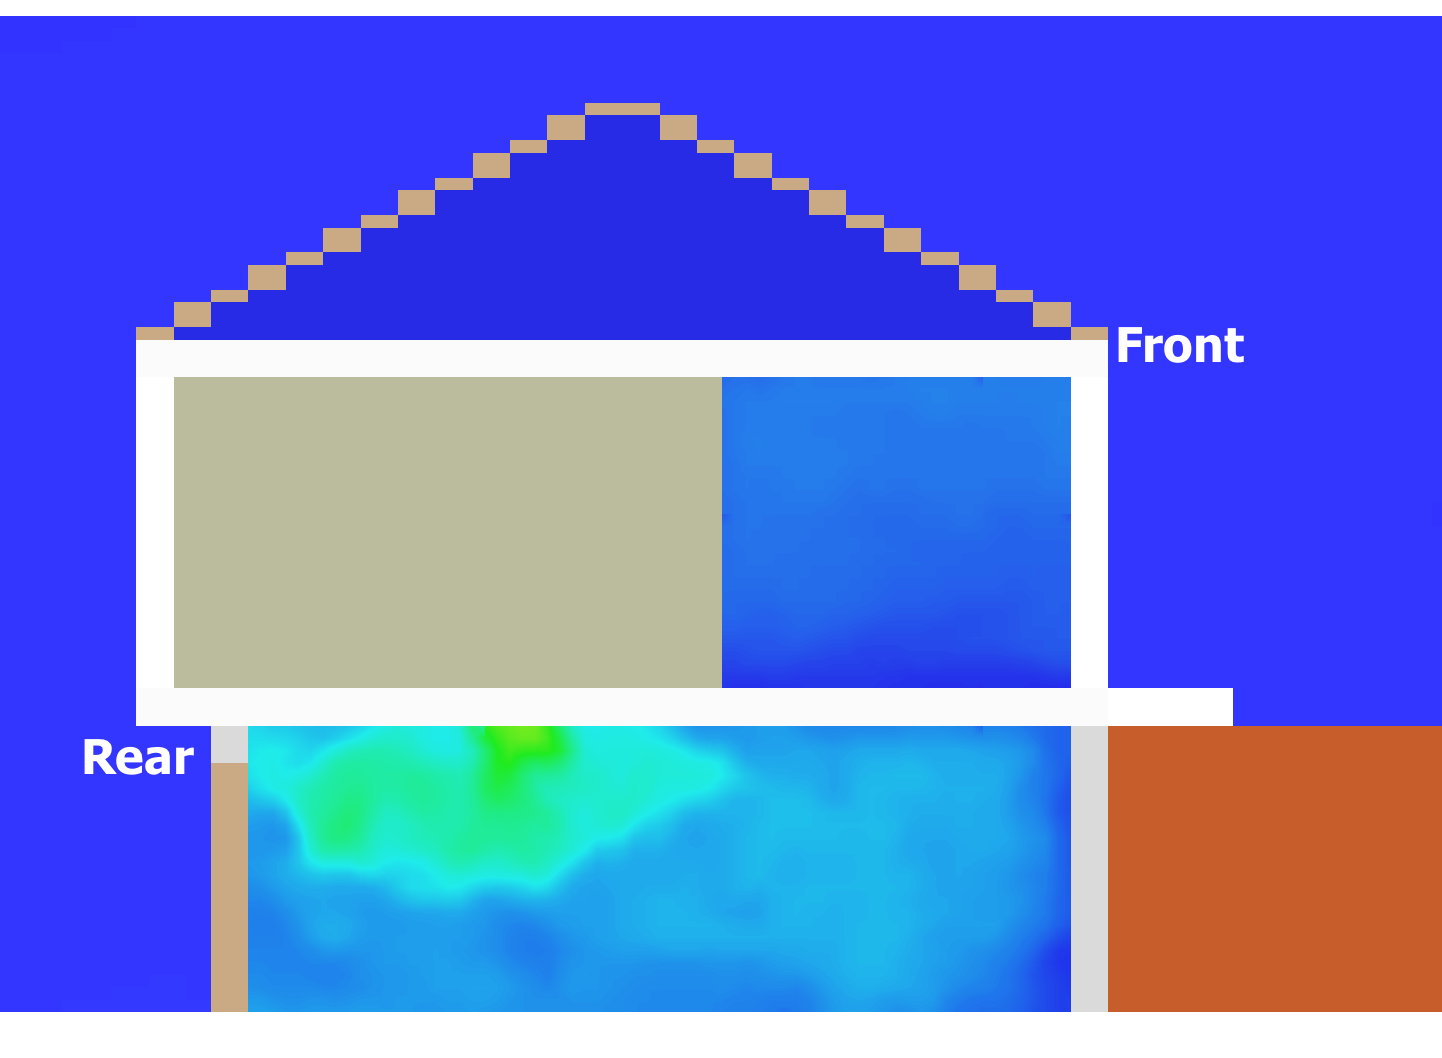
\includegraphics[trim = 0in 0in 0in 0in, clip=true, width=\textwidth]{../Figures/side_view_99s} \\
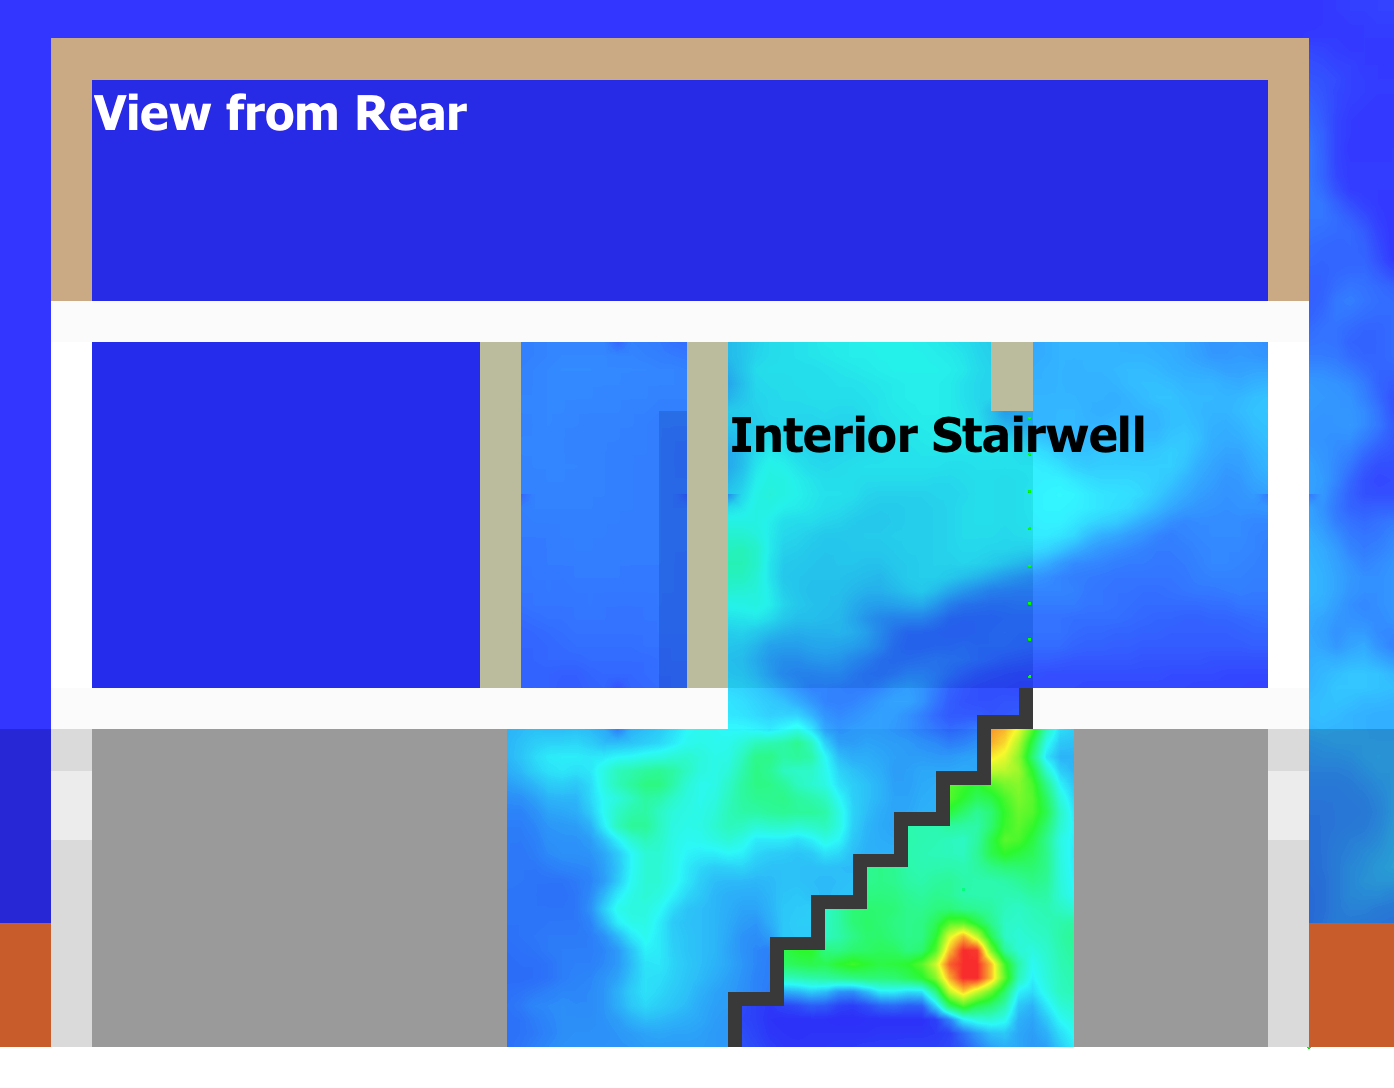
\includegraphics[trim = 0in 0in 0in 0in, clip=true, width=\textwidth]{../Figures/stair_view_99s} 
\end{subfigure}
\begin{subfigure}{0.35\textwidth}
%\documentclass{standalone}
%\usepackage{pgfplots}
%\begin{document}
%\pgfplotsset{
%	colormap={blackwhite}{[5pt]
%		rgb255(0pt)=(0,0,255); 
%		rgb255(100pt)=(0,255,255); 
%		rgb255(200pt)=(0,255,0); 
%		rgb255(300pt)=(255,255,0); 
%		rgb255(400pt)=(255,0,0)
%	},
%}
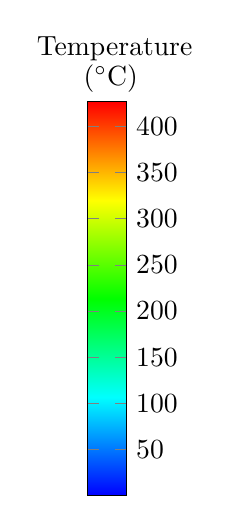
\begin{tikzpicture}
\node at (0.65,0.67) {Temperature};
\node at (0.6,0.3) {($^\circ$C)};
\begin{axis}[
    hide axis,
    scale only axis,
    height=0pt,
    width=0pt,
    colorbar,
    point meta min=0,
    point meta max=426.667,
    colorbar style={
        height=5cm,
        ytick={50,100,...,450}
    }]
    \addplot [draw=none] coordinates {(0,0)};
\end{axis}
\end{tikzpicture}
%\end{document}

%\documentclass{standalone}
%\usepackage{pgfplots}
%\begin{document}
%\pgfplotsset{
%	colormap={blackwhite}{[5pt]
%		rgb255(0pt)=(0,0,255); 
%		rgb255(100pt)=(0,255,255); 
%		rgb255(200pt)=(0,255,0); 
%		rgb255(300pt)=(255,255,0); 
%		rgb255(400pt)=(255,0,0)
%	},
%}
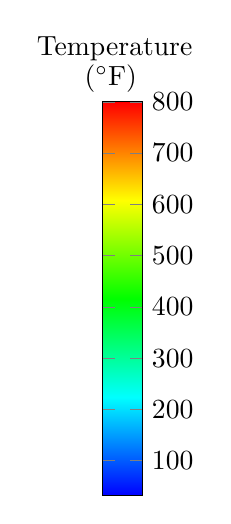
\begin{tikzpicture}
\node at (0.45,0.67) {Temperature};
\node at (0.4,0.3) {($^\circ$F)};
\begin{axis}[
    hide axis,
    scale only axis,
    height=0pt,
    width=0pt,
    colorbar,
    point meta min=32,
    point meta max=800,
    colorbar style={
        height=5cm,
        ytick={100,200,...,800}
    }]
    \addplot [draw=none] coordinates {(0,0)};
\end{axis}
\end{tikzpicture}
%\end{document} \\
\end{subfigure}
\caption[Interior temperature contours 1~s before front door was opened]
{Interior temperature contours 1~s before front door was opened. The top snapshot shows temperatures on the first floor and basement on a plane that runs through the center front door. The bottom snapshot shows temperatures on the first floor and basement on a plane that runs through the center of the interior stairwell doorway.}
\label{fig:int_temp_99s}
\end{figure}

\begin{figure}[!ht]
\begin{subfigure}{0.65\textwidth}
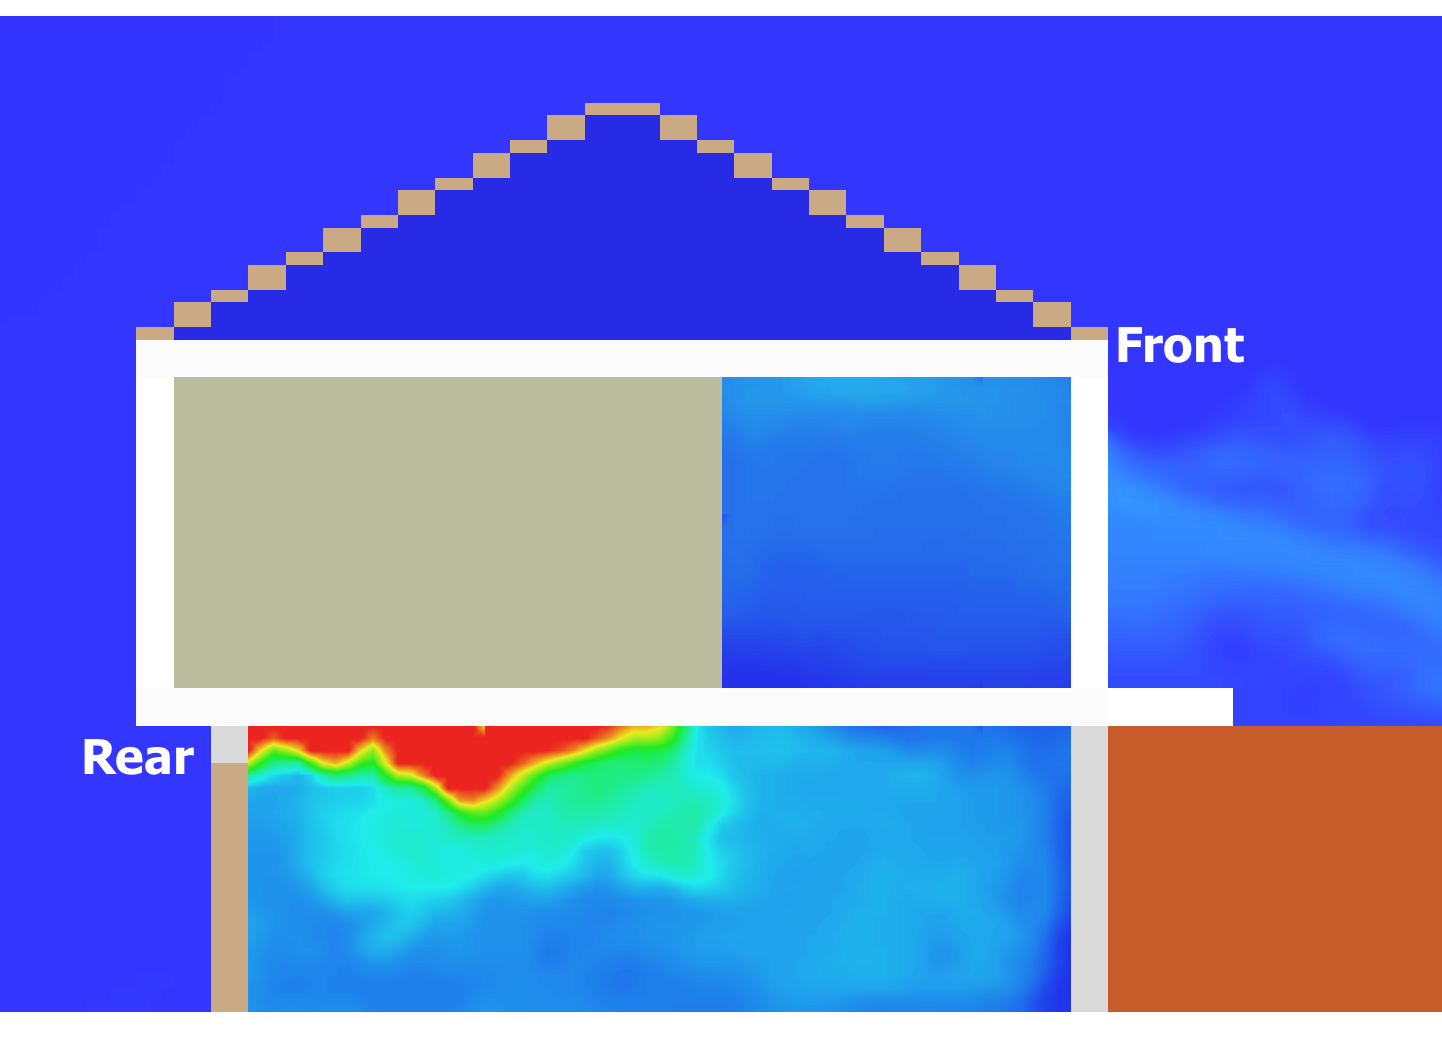
\includegraphics[trim = 0in 0in 0in 0in, clip=true, width=\textwidth]{../Figures/side_view_101s} \\
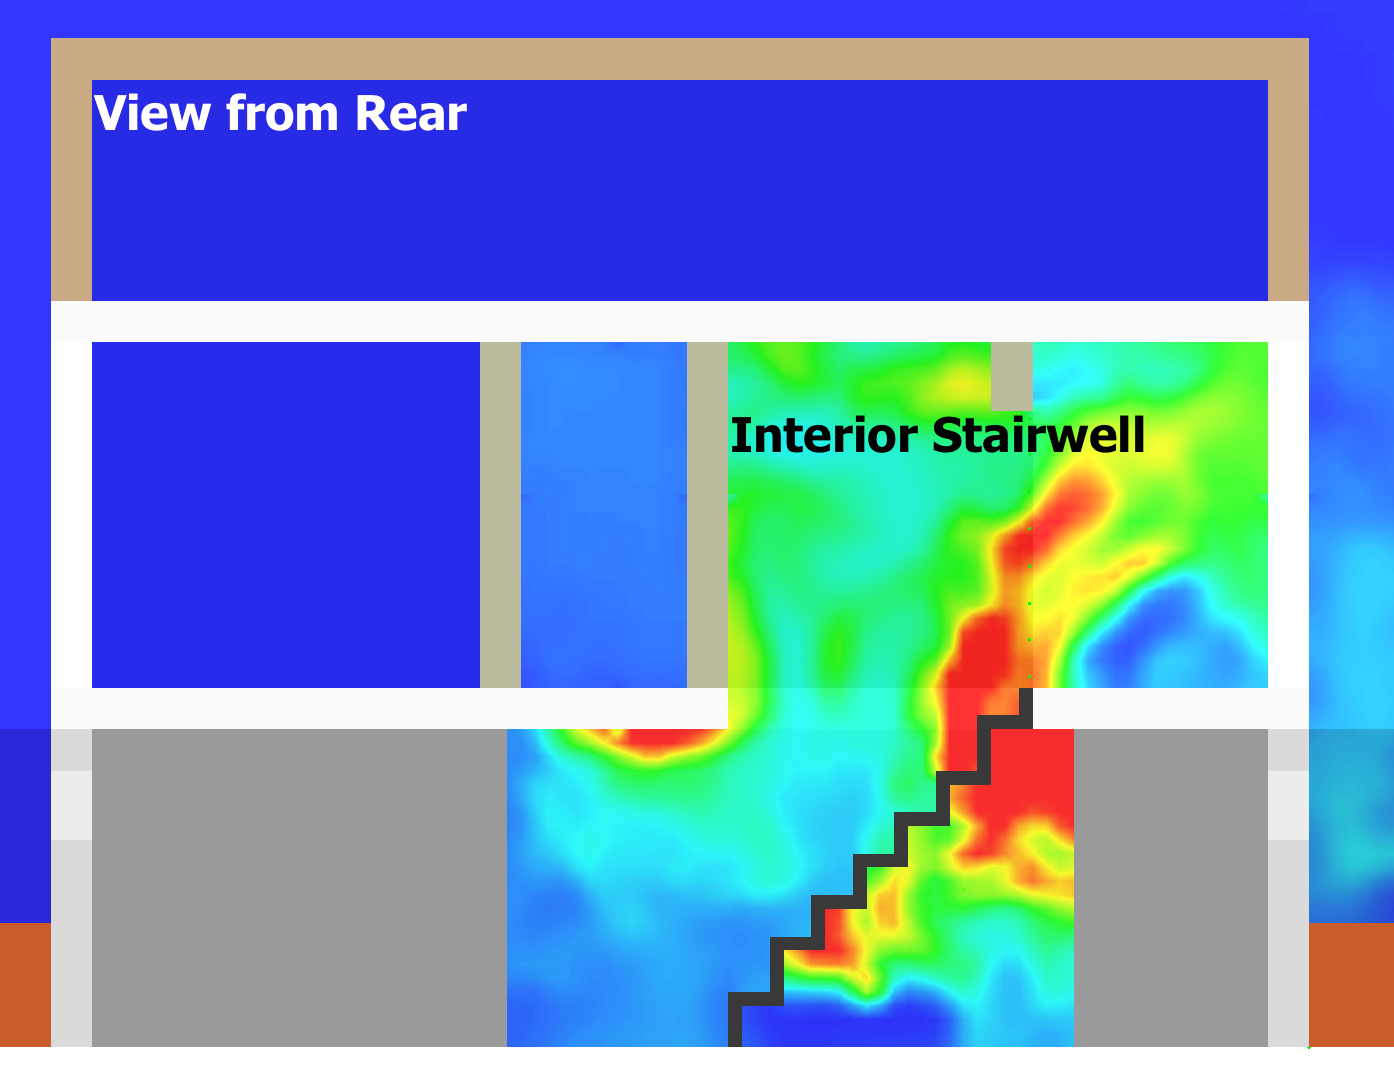
\includegraphics[trim = 0in 0in 0in 0in, clip=true, width=\textwidth]{../Figures/stair_view_101s} 
\end{subfigure}
\begin{subfigure}{0.35\textwidth}
%\documentclass{standalone}
%\usepackage{pgfplots}
%\begin{document}
%\pgfplotsset{
%	colormap={blackwhite}{[5pt]
%		rgb255(0pt)=(0,0,255); 
%		rgb255(100pt)=(0,255,255); 
%		rgb255(200pt)=(0,255,0); 
%		rgb255(300pt)=(255,255,0); 
%		rgb255(400pt)=(255,0,0)
%	},
%}
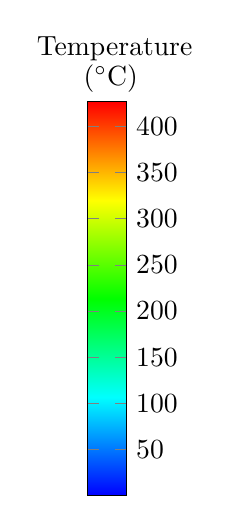
\begin{tikzpicture}
\node at (0.65,0.67) {Temperature};
\node at (0.6,0.3) {($^\circ$C)};
\begin{axis}[
    hide axis,
    scale only axis,
    height=0pt,
    width=0pt,
    colorbar,
    point meta min=0,
    point meta max=426.667,
    colorbar style={
        height=5cm,
        ytick={50,100,...,450}
    }]
    \addplot [draw=none] coordinates {(0,0)};
\end{axis}
\end{tikzpicture}
%\end{document}

%\documentclass{standalone}
%\usepackage{pgfplots}
%\begin{document}
%\pgfplotsset{
%	colormap={blackwhite}{[5pt]
%		rgb255(0pt)=(0,0,255); 
%		rgb255(100pt)=(0,255,255); 
%		rgb255(200pt)=(0,255,0); 
%		rgb255(300pt)=(255,255,0); 
%		rgb255(400pt)=(255,0,0)
%	},
%}
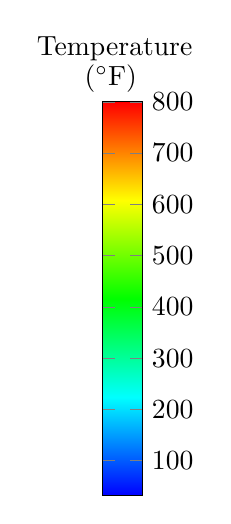
\begin{tikzpicture}
\node at (0.45,0.67) {Temperature};
\node at (0.4,0.3) {($^\circ$F)};
\begin{axis}[
    hide axis,
    scale only axis,
    height=0pt,
    width=0pt,
    colorbar,
    point meta min=32,
    point meta max=800,
    colorbar style={
        height=5cm,
        ytick={100,200,...,800}
    }]
    \addplot [draw=none] coordinates {(0,0)};
\end{axis}
\end{tikzpicture}
%\end{document} \\
\end{subfigure}
\caption[Interior temperature contours 1~s after front door was opened]
{Interior temperature contours 1~s after front door was opened. The top snapshot shows temperatures on the first floor and basement on a plane that runs through the center front door. The bottom snapshot shows temperatures on the first floor and basement on a plane that runs through the center of the interior stairwell doorway.}
\label{fig:int_temp_101s}
\end{figure}

\begin{figure}[!ht]
\begin{subfigure}{0.65\textwidth}
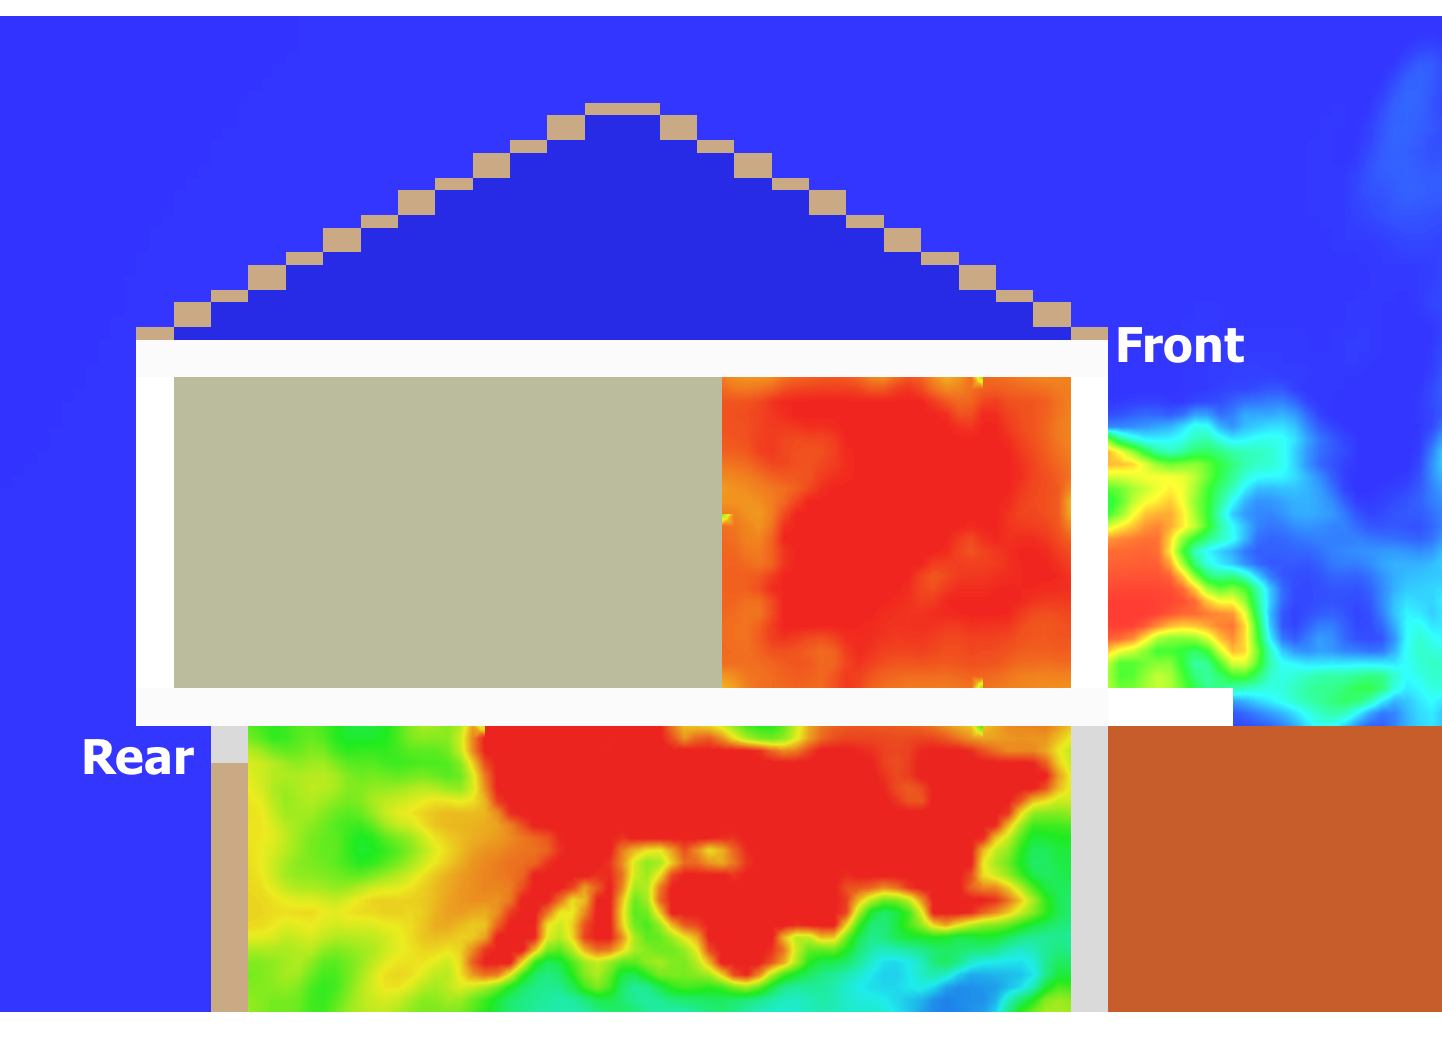
\includegraphics[trim = 0in 0in 0in 0in, clip=true, width=\textwidth]{../Figures/side_view_142s} \\
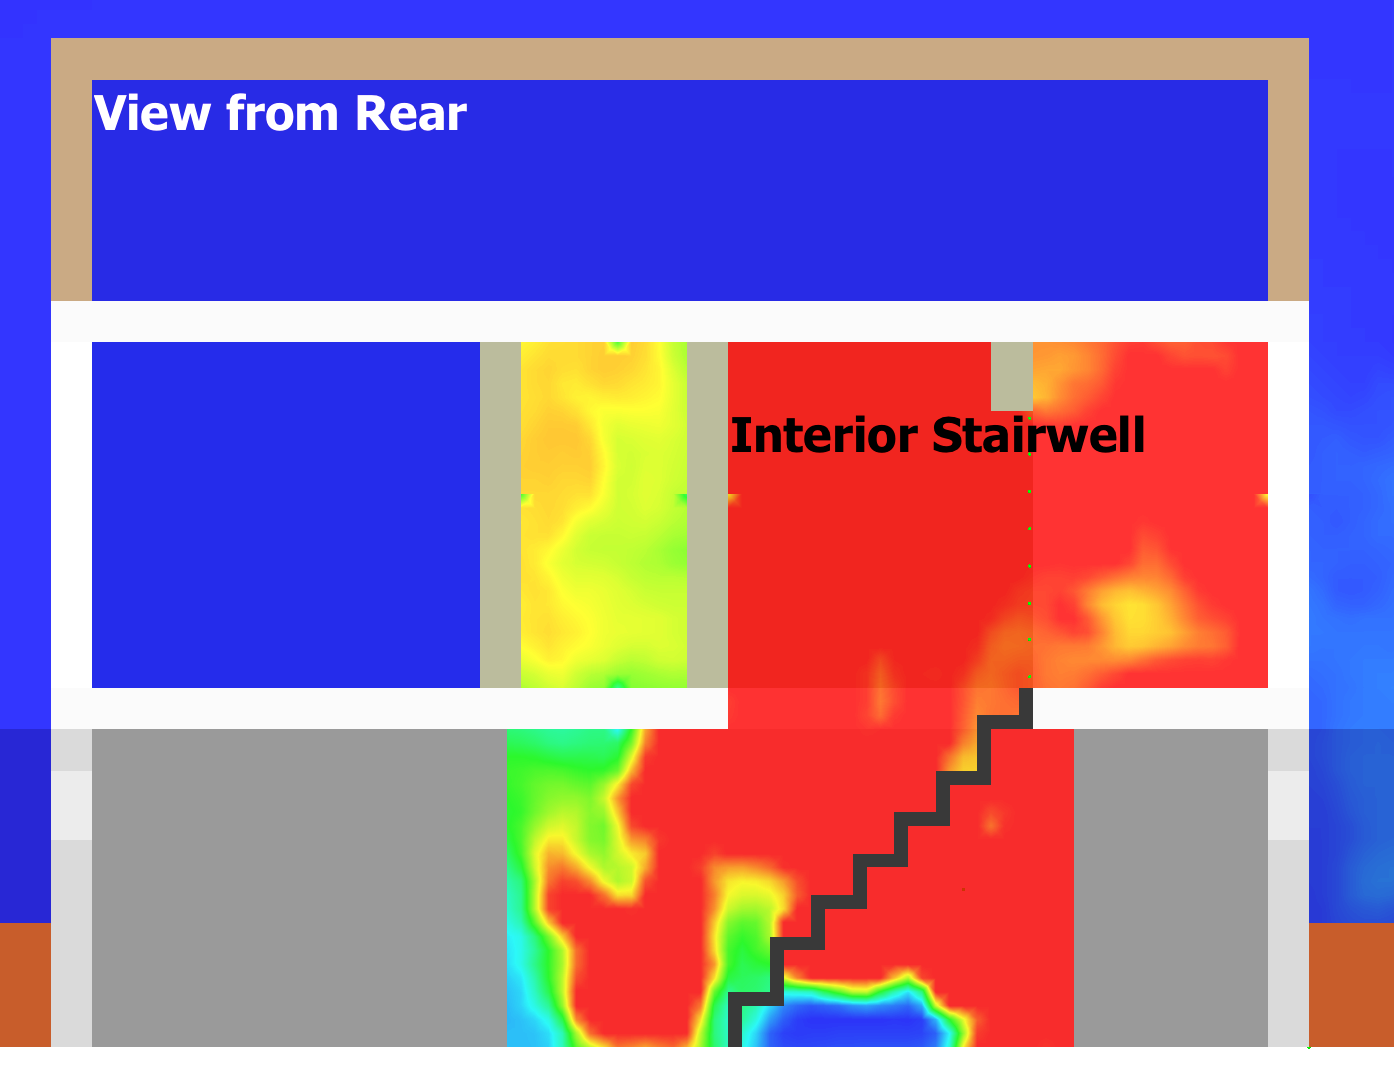
\includegraphics[trim = 0in 0in 0in 0in, clip=true, width=\textwidth]{../Figures/stair_view_142s} 
\end{subfigure}
\begin{subfigure}{0.35\textwidth}
%\documentclass{standalone}
%\usepackage{pgfplots}
%\begin{document}
%\pgfplotsset{
%	colormap={blackwhite}{[5pt]
%		rgb255(0pt)=(0,0,255); 
%		rgb255(100pt)=(0,255,255); 
%		rgb255(200pt)=(0,255,0); 
%		rgb255(300pt)=(255,255,0); 
%		rgb255(400pt)=(255,0,0)
%	},
%}
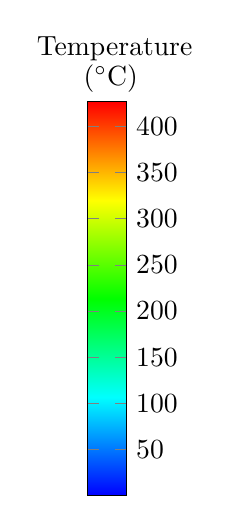
\begin{tikzpicture}
\node at (0.65,0.67) {Temperature};
\node at (0.6,0.3) {($^\circ$C)};
\begin{axis}[
    hide axis,
    scale only axis,
    height=0pt,
    width=0pt,
    colorbar,
    point meta min=0,
    point meta max=426.667,
    colorbar style={
        height=5cm,
        ytick={50,100,...,450}
    }]
    \addplot [draw=none] coordinates {(0,0)};
\end{axis}
\end{tikzpicture}
%\end{document}

%\documentclass{standalone}
%\usepackage{pgfplots}
%\begin{document}
%\pgfplotsset{
%	colormap={blackwhite}{[5pt]
%		rgb255(0pt)=(0,0,255); 
%		rgb255(100pt)=(0,255,255); 
%		rgb255(200pt)=(0,255,0); 
%		rgb255(300pt)=(255,255,0); 
%		rgb255(400pt)=(255,0,0)
%	},
%}
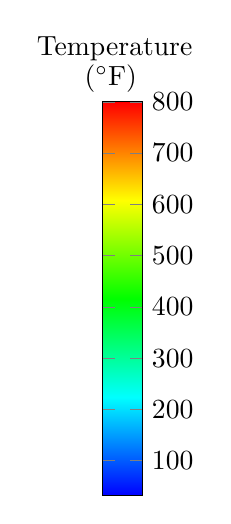
\begin{tikzpicture}
\node at (0.45,0.67) {Temperature};
\node at (0.4,0.3) {($^\circ$F)};
\begin{axis}[
    hide axis,
    scale only axis,
    height=0pt,
    width=0pt,
    colorbar,
    point meta min=32,
    point meta max=800,
    colorbar style={
        height=5cm,
        ytick={100,200,...,800}
    }]
    \addplot [draw=none] coordinates {(0,0)};
\end{axis}
\end{tikzpicture}
%\end{document} \\
\end{subfigure}
\caption[Interior temperature contours as firefighters made entry to the structure]
{Interior temperature contours as firefighters made entry to the structure. The top snapshot shows temperatures on the first floor and basement on a plane that runs through the center front door. The bottom snapshot shows temperatures on the first floor and basement on a plane that runs through the center of the interior stairwell doorway.}
\label{fig:int_temp_142s}
\end{figure}

Based on these results and the simulation results shown in Sections~\ref{velocity} and \ref{temp}, after the front door was opened, the simulated flow path temperatures in the interior stairwell were in excess of 400~$^{\circ}$C (750~$^{\circ}$F) and the flow velocities were in excess of 9 m/s (20 mph). The conditions in the interior stairwell changed from tenable to high-hazard very rapidly following the opening of the front door. Within the structure, the hot gases and smoke were moving along the flow path from the basement towards the door located on the front side of the structure via the interior stairwell. The simulated temperatures are consistent with the post-incident conditions that were documented in the interior stairwell.

Ongoing research and experimental work is being conducted by NIST to gain a better understanding of convective heat transfer to firefighter personal protective equipment, including firefighting gear, helmets, self-contained breathing apparatuses, etc. The goal of this ongoing research is to parameterize various flow path conditions (elevated temperatures and velocities) and determine their effect on the rate of heat transfer and amount of energy storage in firefighting safety equipment.

\clearpage

\section{Tactical Considerations}
\label{tactical_considerations}

In this fire incident, the initial failure of the basement windows with strong incident winds on the rear side of the structure coincided with a rapid change in the thermal conditions in the interior stairwell and first floor after the front door to the structure was opened. The open front door resulted in the establishment of a flow path within the interior stairwell with highly hazardous conditions. These conditions would be equivalent to or greater than a Class~III exposure~\cite{Donnelly2006}.

The interior stairwell acted as a chimney for hot gases in the basement to flow towards regions of lower pressure and vent openings located on the front side of the structure. Firefighters should avoid placing themselves within a flow path where elevated temperatures and flow velocities can present hazardous conditions and increase the rate of heat transfer to firefighting gear via convection. A 360$^\circ$ scene size-up by arriving firefighters can help determine the location of the fire and identify potential flow paths within a structure. Door control can also be used to avoid creating inlet and outlet vents that could result in the establishment of a flow path.

Fire suppression efforts should be coordinated with interior operations and ventilation procedures to reduce thermal hazards related to flow paths within a structure. Ongoing research by NIST, Underwriters Laboratories (UL), and others has demonstrated that applying water from the exterior into the fire area of a structure (prior to the start of interior operations) can significantly improve the safety of firefighters by reducing the thermal hazard from the fire and reducing the potential for developing high velocity hot gas flows within the structure~\cite{madrzykowski2009fire, kerber2009fire}.

There have been many previous fire incidents~\cite{NIOSH:Pettit,NIOSH:Washenitz,NIOSH:Mezzanotte,NIOSH:McFall,NIOSH:McFall2,NIOSH:McFall3,NIOSH:Berardinelli,NIOSH:Koedam,NIOSH:McFall4,NIOSH:Tarley,NIOSH:Braddee,NIOSH:Merinar,NIOSH:Bowyer2,NIOSH:Loflin,NIOSH:Bowyer} in which changes in the flow paths are thought to have had an adverse impact on firefighter and occupant safety. Table~\ref{tab:LODD} lists the NIOSH investigation reports from the past 15 years in which it could be determined that a flow path played a role in the related incident. This table lists the NIOSH report number, the outcome, and a brief description of the flow path details.

Based on a review of these incidents, it is clear that fires with rapidly developing or changing flow paths are a significant hazard to the fire service. The development of (or changes to) a flow path could be caused by the failure of a component of the structure, such as a door, window, or portion of a ceiling, wall or floor. Environmental conditions such as wind can generate hazardous thermal conditions within a flow path. Uncoordinated ventilation procedures can also be the cause of increased thermal hazards within a flow path.

\begin{table}[!ht]
\caption[Flow path related LODD/LODI incidents]
{Flow path related LODD/LODI incidents}
\begin{tabular}{lll}
\toprule
NIOSH Report No. & No. of LODDs/LODIs & Flow Path Details                                              \\
\midrule
99-F01   \cite{NIOSH:Pettit}        &  3 LODDs            &  From apartment into hallway on 10th       \\
                                    &                     &  floor of high-rise apartment building     \\
99-F21   \cite{NIOSH:Washenitz}     &  2 LODDs            &  Basement to 1st floor                     \\
                                    &  2 LODIs            &                                            \\
F2000-04 \cite{NIOSH:Mezzanotte}    &  3 LODDs            &  1st floor to 2nd floor                    \\
                                    &  3 civilian deaths  &                                            \\
F2000-16 \cite{NIOSH:McFall}        &  1 LODD             &  2nd floor hallway through                 \\
                                    &  1 LODI             &  2nd floor apartment                       \\
                                    &  1 civilian death   &                                            \\
F2000-23 \cite{NIOSH:McFall2}       &  1 LODD             &  From ground level to 1st floor then to    \\
                                    &  2 LODIs            &  2nd floor, flow exited through ceiling    \\
F2000-43 \cite{NIOSH:McFall3}       &  1 serious LODI     &  1st floor to 2nd floor                    \\
                                    &  2 other LODIs      &                                            \\
F2004-02 \cite{NIOSH:Berardinelli}  &  1 LODD             &  1st floor to basement                     \\
F2005-02 \cite{NIOSH:Koedam}        &  1 LODD             &  Rear to front of the building             \\
                                    &  4 LODIs            &                                            \\
F2005-04 \cite{NIOSH:McFall4}       &  1 LODD             &  Basement to 1st floor                     \\
                                    &  9 LODIs            &                                            \\
F2007-09 \cite{NIOSH:Tarley}        &  1 LODD             &  3 story training burn - flow through      \\
                                    &  2 LODIs            &  all levels                                \\
F2007-35 \cite{NIOSH:Braddee}       &  4 LODIs            &  1st floor to 2nd floor                    \\
F2009-11 \cite{NIOSH:Merinar}       &  2 LODDs            &  Rear to front of the building             \\
F2011-13 \cite{NIOSH:Bowyer2}       &  2 LODDs            &  Lower level up stairs and through         \\
                                    &                     &  entry door and garage                     \\
F2011-31 \cite{NIOSH:Loflin}        &  1 LODD             &  Fire extended from lower level apartment  \\
F2012-28 \cite{NIOSH:Bowyer}        &  1 LODD             &  Attic fire extended into closed           \\
                                    &  1 LODI             &  porch and then into 2nd floor             \\
\bottomrule
\end{tabular}
\label{tab:LODD}
\end{table}

\clearpage

\chapter{Summary}
Fire Dynamics Simulator was used to provide insight into the fire dynamics of a fire that occurred within a single-story plus basement, single-family residential structure in Riverdale Heights, MD, that resulted in the serious injury of two firefighters. The fuel, fire size, and fire growth rate that were used in the FDS simulation were estimated by taking into account all of the available information including the post incident report from Prince George's Country Fire/EMS~\cite{PGCounty2013}, post-incident pictures, and relevant literature. This resulted in a maximum specified source fire of approximately 8.5~MW in the basement. Based on the limited ventilation conditions in the basement, the FDS simulation results indicated that before the front door was opened, there was combustion occurring outside the structure at the rear basement windows which had failed prior to arrival. Once the front door was opened, there was sufficient oxygen for combustion to occur within the structure, which intermittent flaming combustion on the first floor.

The fire originated in the basement, and the interior stairwell acted as a chimney for hot gases in the basement to flow towards regions of lower pressure through the open front door of the structure. After the front door was opened, a flow path was established between the basement and the front side of the structure (the front door). The opening of the front door resulted in a rapid change in the conditions within the flow path. In the interior stairwell, the flow velocities were greater than 9~m/s (20~mph) and the temperature of the gases was estimated to be in excess of 400~$^{\circ}$C (750~$^{\circ}$F), which exceeds the Class III exposure temperature of 260~$^{\circ}$C (500~$^{\circ}$F).

Two firefighters were located in the flow path between the basement and the doors on the front side of the structure. One firefighter was able to break a window to escape the hazardous conditions and after a call for assistance the second firefighter was removed from the structure and immediate medical treatment was provided. The two firefighters were transported to the local medical center where they were treated for their injuries. Four other firefighters were injured on-scene and transported to the hospital for treatment.

\chapter{Acknowledgments}

The authors would like to thank XXXXX of the Prince George's County Fire/EMS Department for their assistance with this study and their dedication to improving firefighter safety. The authors would also like to thank John Culbertson, Director of the Montana Fire Services Training School, for his assistance in researching and compiling the flow path related LODD/LODI incidents shown in Table~\ref{tab:LODD}. Finally, the authors would like to thank Joseph Willi of the University of Illinois Urbana-Champaign for his assistance in creating dimensioned drawings of the structure.


\bibliography{../../../Bibliography/FDS_refs,../../../Bibliography/FDS_general}

\appendix

\chapter{Dimensioned Drawings}
\label{app_draw}

\begin{figure}[!ht]
\centering
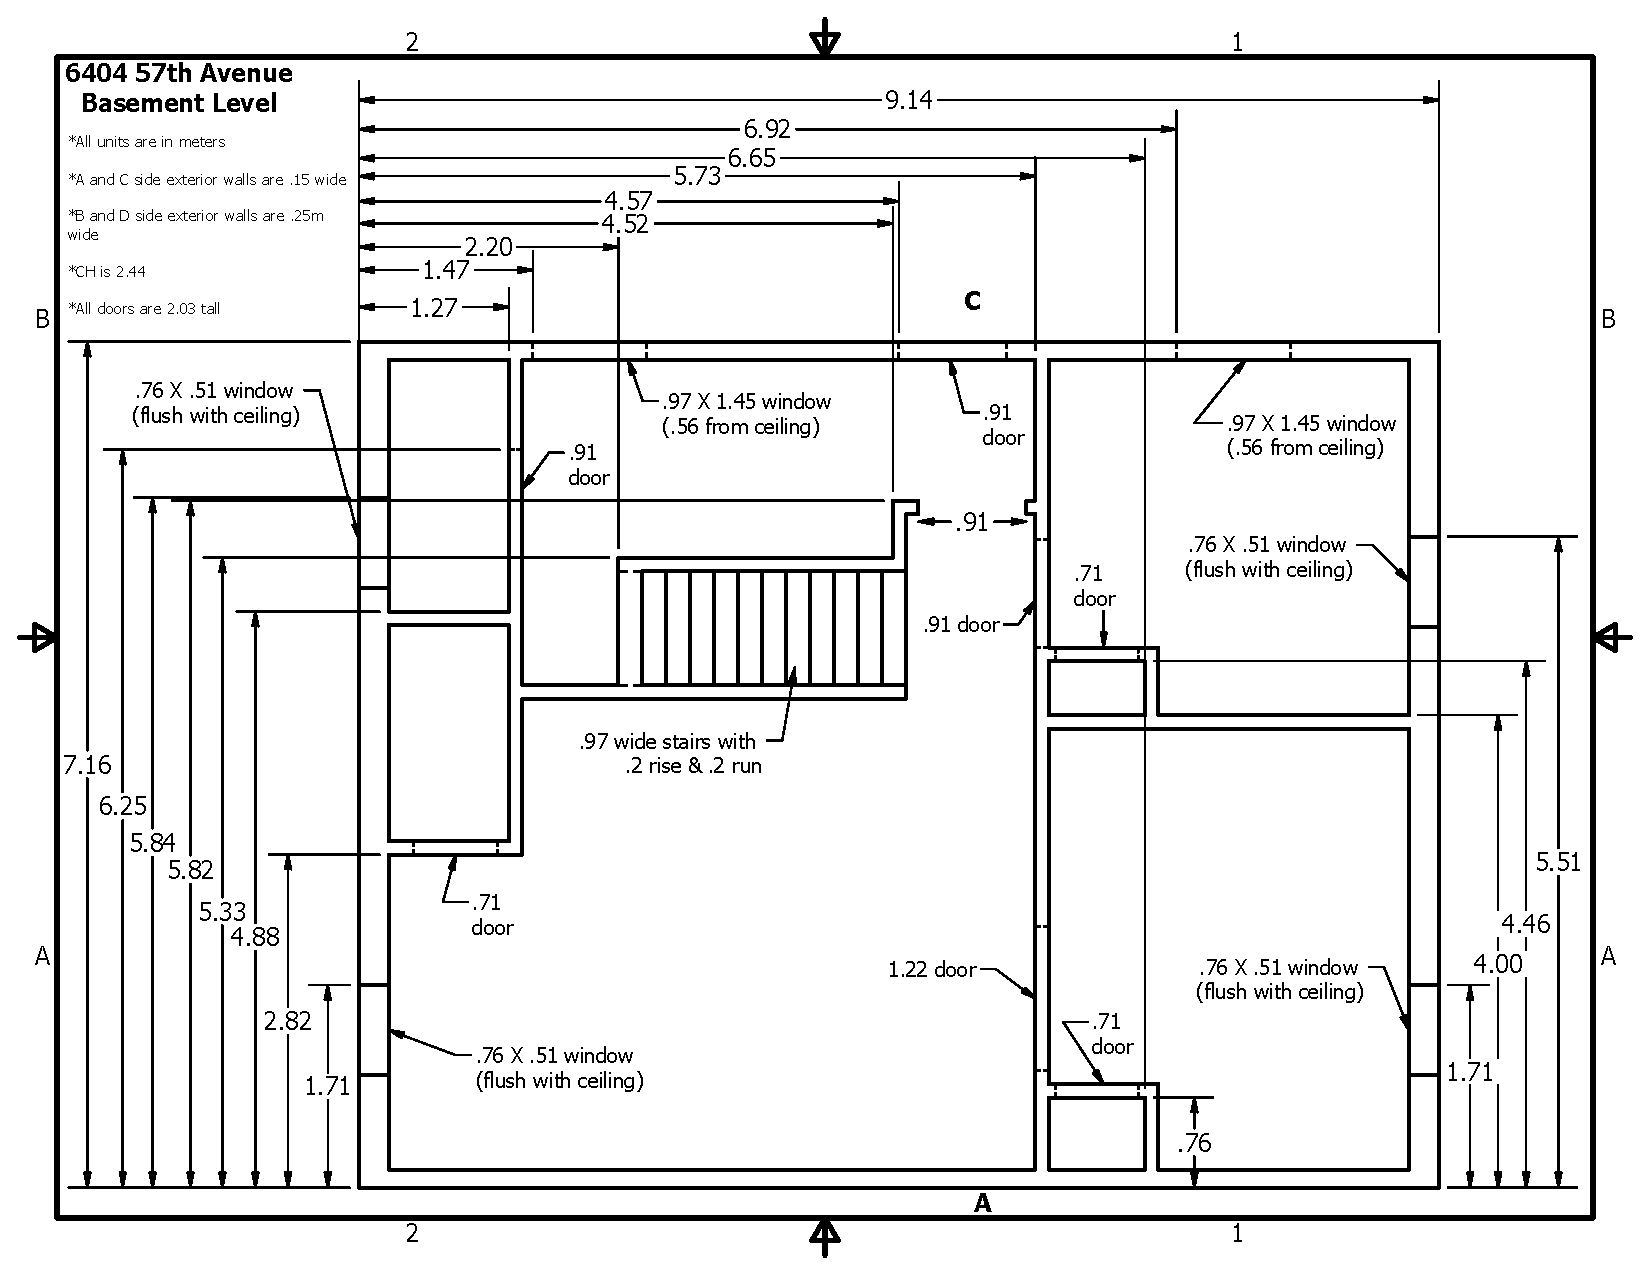
\includegraphics[width=1\textwidth]{../Figures/Basement_Metric}
\caption[Dimensioned drawing of first floor.]{Dimensioned drawing of the basement. The measurements are accurate to within 15~cm (6~in).}
\label{fig:basement}
\end{figure}

\begin{figure}[!ht]
\centering
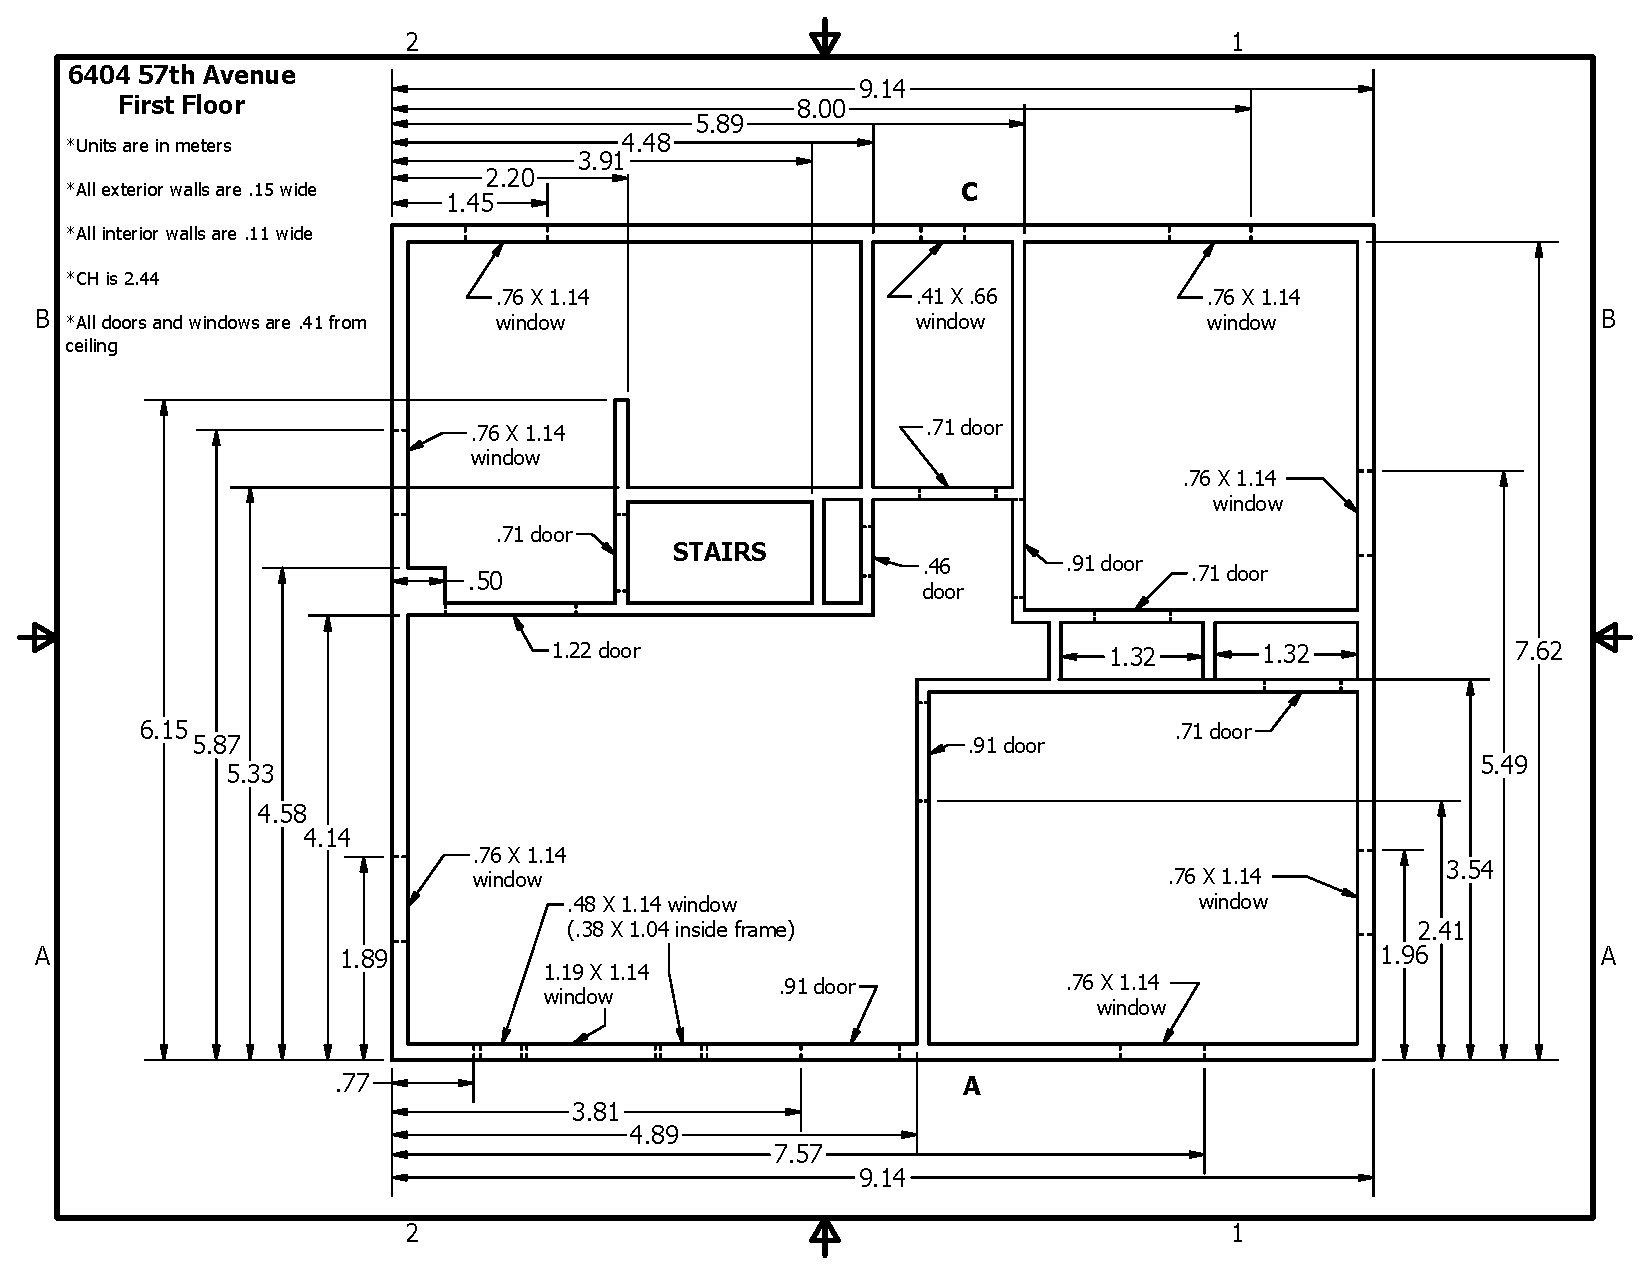
\includegraphics[width=1\textwidth]{../Figures/First_Floor_Metric}
\caption[Dimensioned drawing of second floor.]{Dimensioned drawing of the first floor. The measurements are accurate to within 15~cm (6~in).}
\label{fig:first_floor}
\end{figure}


\end{document}
